\documentclass[a4paper]{article}

\usepackage{bm}
\usepackage{sidecap}
\usepackage{tabularx}
% \usepackage{hyperref}
\usepackage[margin=1in]{geometry}


\usepackage{graphicx}

% \setkeys{Gin}{width=\linewidth,totalheight=\textheight,keepaspectratio}
% \graphicspath{{graphics/}}

\usepackage{sectsty}
\sectionfont{\fontsize{14.4}{18}\selectfont}
\subsectionfont{\fontsize{14}{17}\selectfont}
\subsubsectionfont{\fontsize{12}{14.4}\selectfont}

\title{\textbf{ 
        \Large {Operation Manual for} \\ 
        \vspace {10pt}
        \Huge {P$\bm{\mu}$SL 3D-Printer } \\
        \vspace {10pt}
        \LARGE {in portable mode}	\\
        \vspace {10pt}
        \Large{(McKay 304)}
        \vspace {20pt}
}}
\author{\textit{Tianyu Gu} \\
    \textit{Sicong Shan} \\
\textit{Bertoldi Group}}
% \date{}

\begin{document}

\maketitle
\vspace{50pt}

\centering
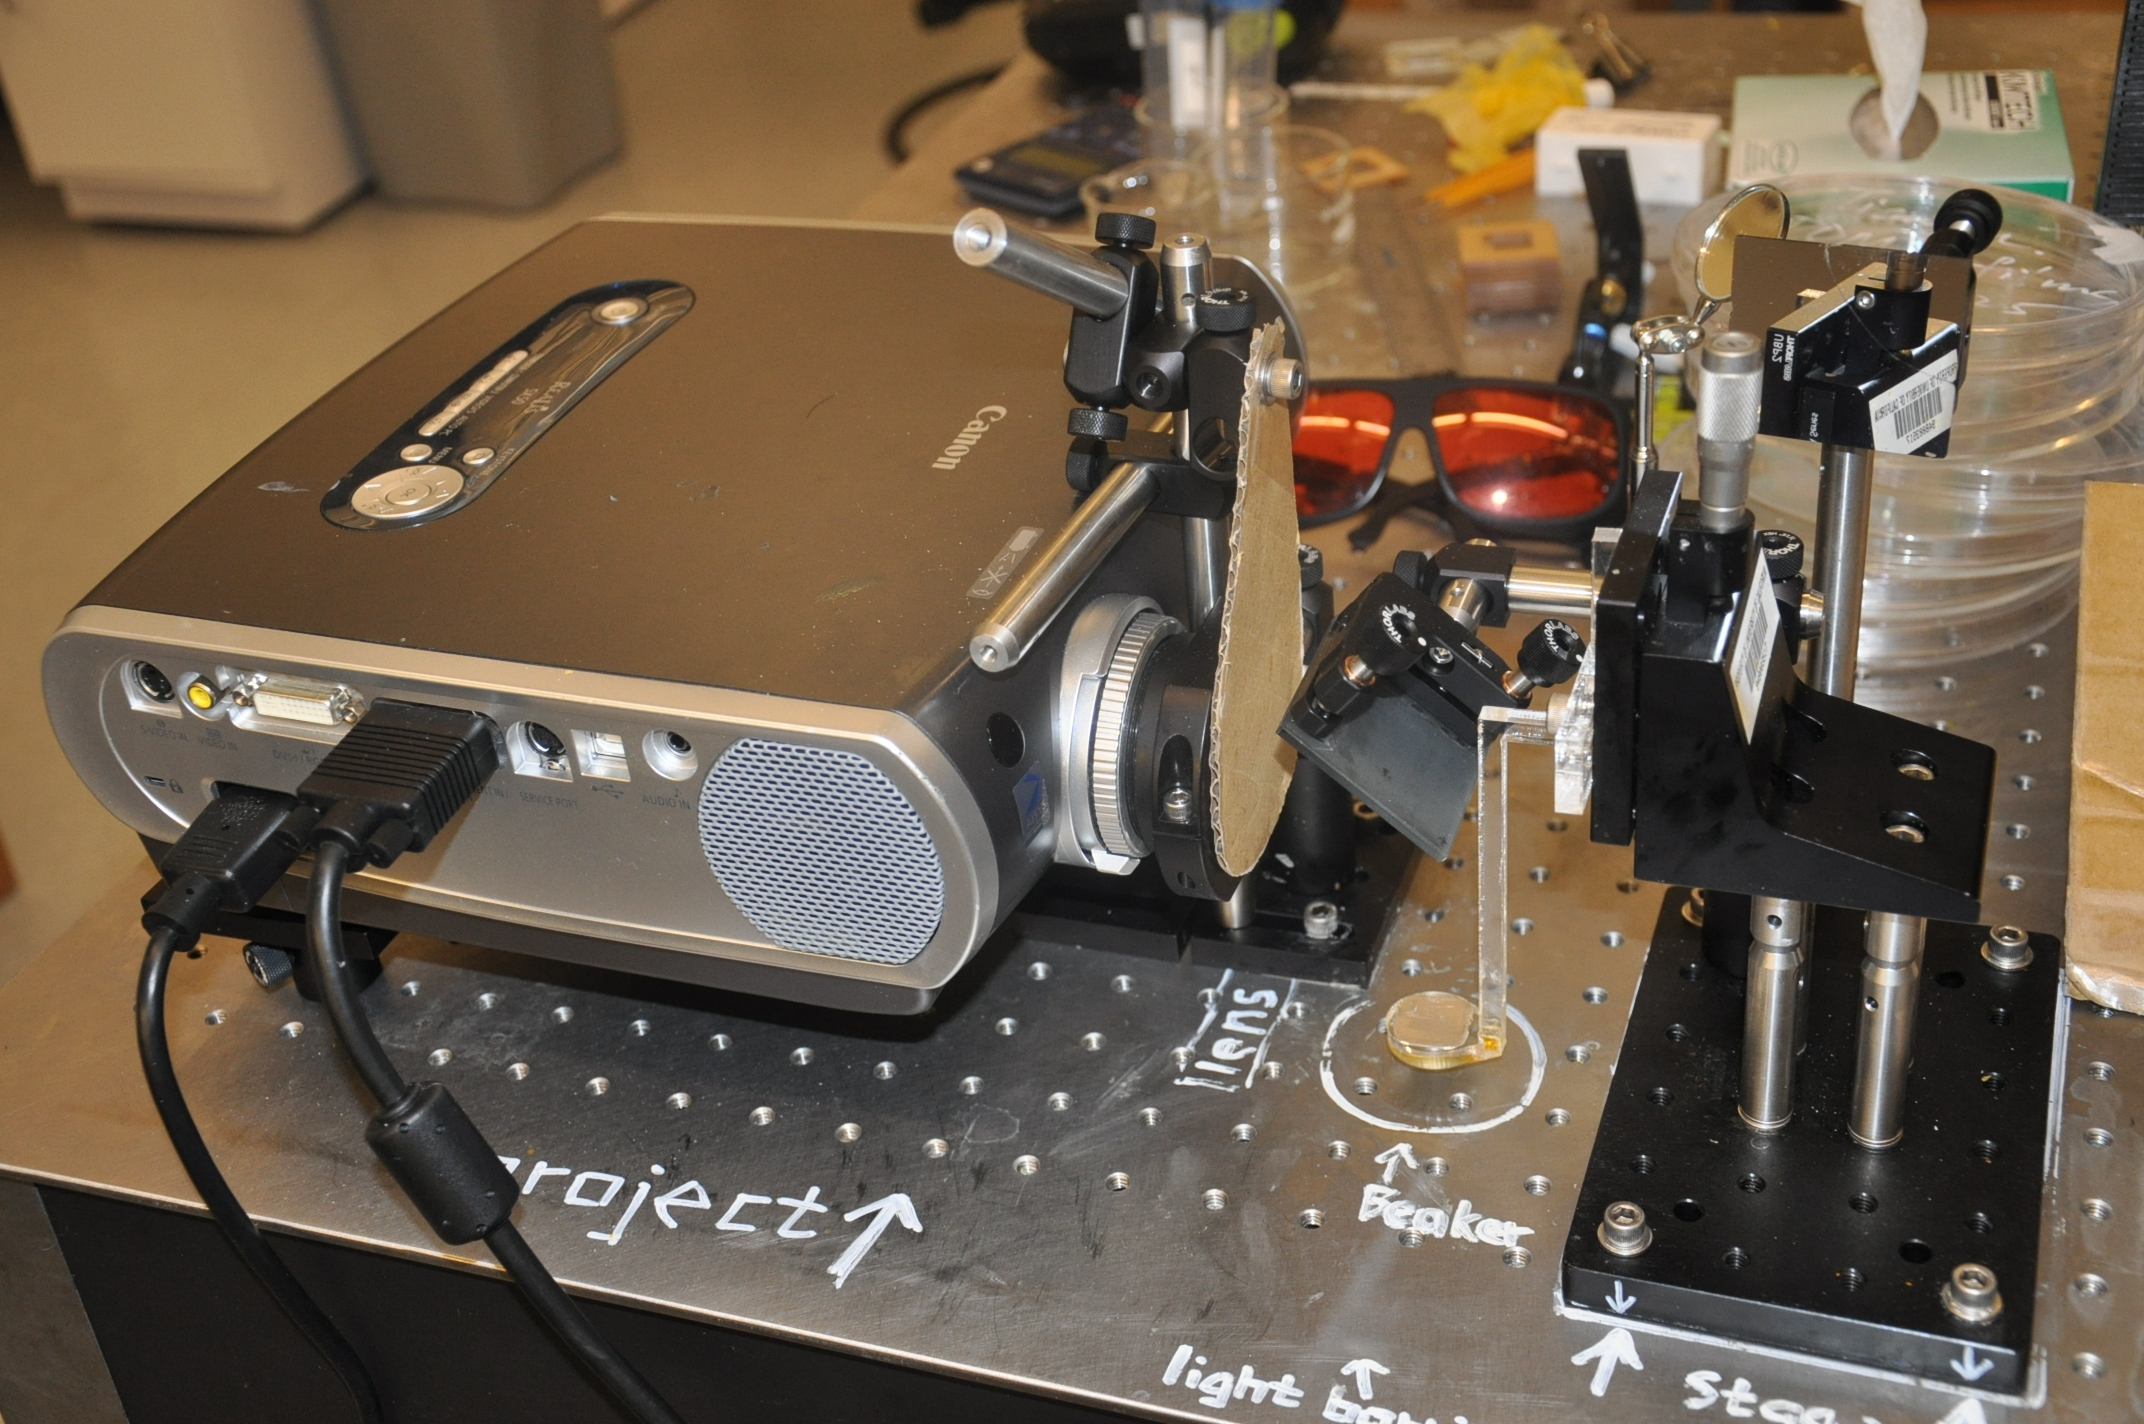
\includegraphics[width=400pt]{frontpic.jpg}
\clearpage

\tableofcontents 
\clearpage

\raggedright

\section{Device Introduction}\label{sec:device-introduction}
The projection microstereolithography (P$\mu$SL) a novel freeform 3D micro-fabrication technology 
which is capable of rapidly fabricating highly complex 3D microstructures in a layer-by-layer fashion. 
This device use a digital data projector and simple optical components like a convex lens and a mirror. 
Image will be projected on the photosensitive resin surface, polymerizing liquid resin into a desired 
3D solid structure. \\ 
\vspace{10pt}

This device is a minimum system of projection micro stereolithography (P$\mu$SL) 3D-printer, adopting the
technology from Howon Jove \footnote{http://www.jove.com/video/4457/micro-3d-printing-using-digital-projector-its-application-study-soft}.
The devcie is with low resolution (about 200$\mu$m) but very easy operation and large printing area. 
It's built for testing the characteristic of new materials like curing time, curing depth, fluidity and so on. \\
\vspace{10pt}

In this section, I will introduce the hardware, the software and the materials we used for the device. \\

\vspace{20pt}

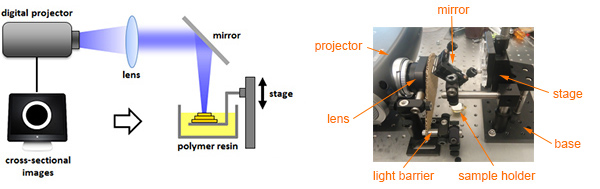
\includegraphics[width=\textwidth]{main.jpg}

\subsection{Hardware}\label{sec:hardware}
\vspace{10pt}

\subsubsection{projector}\label{sec:projector}
\begin{tabularx}{\textwidth}{ cX }
    \raisebox{-0.9\height}{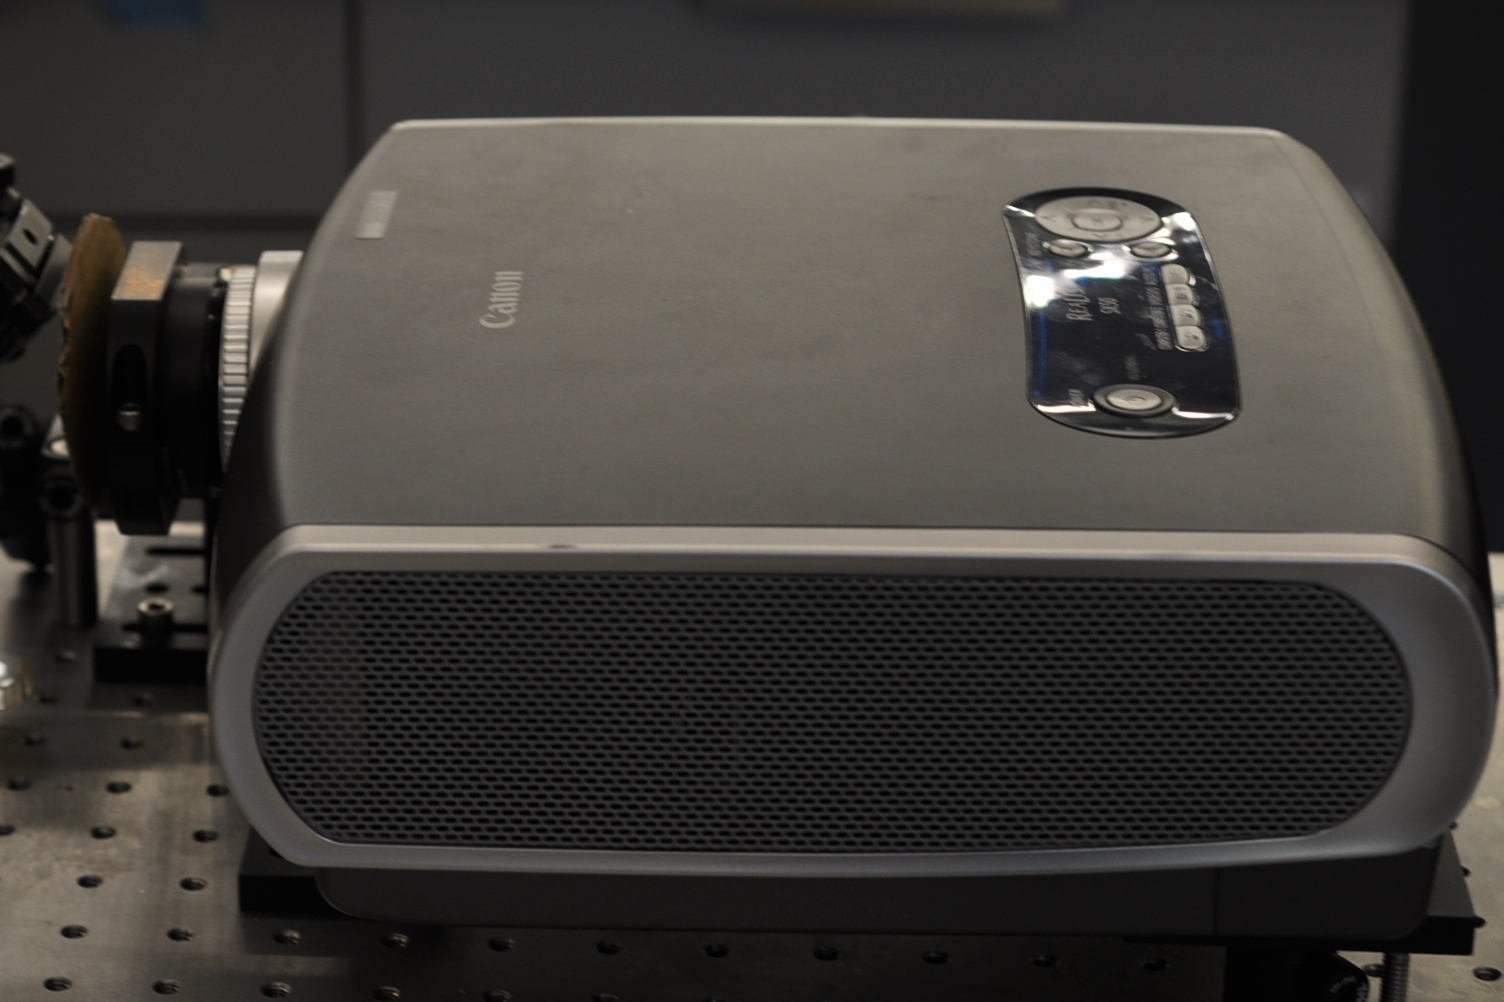
\includegraphics[width=0.33\textwidth]{intro1-1-1.jpg}} &
    The projector is core part of the device. It is connected to the computer and the 
    desktop background will be projected out. Just change the background when you want to be project different 
    images. \textbf{Push the power button} \footnote{The core actions will be printed in bold font.} to turn on 
    the projector and \textbf{double-push} to turn it off. \textbf{Rotating the ring} on the projector lens can 
    adjusting the focial length and making the image sharper. 
\end{tabularx}

\subsubsection{Convex Lens}\label{sec:convex-lens}
\begin{tabularx}{\textwidth}{ cX }
    \raisebox{-0.9\height}{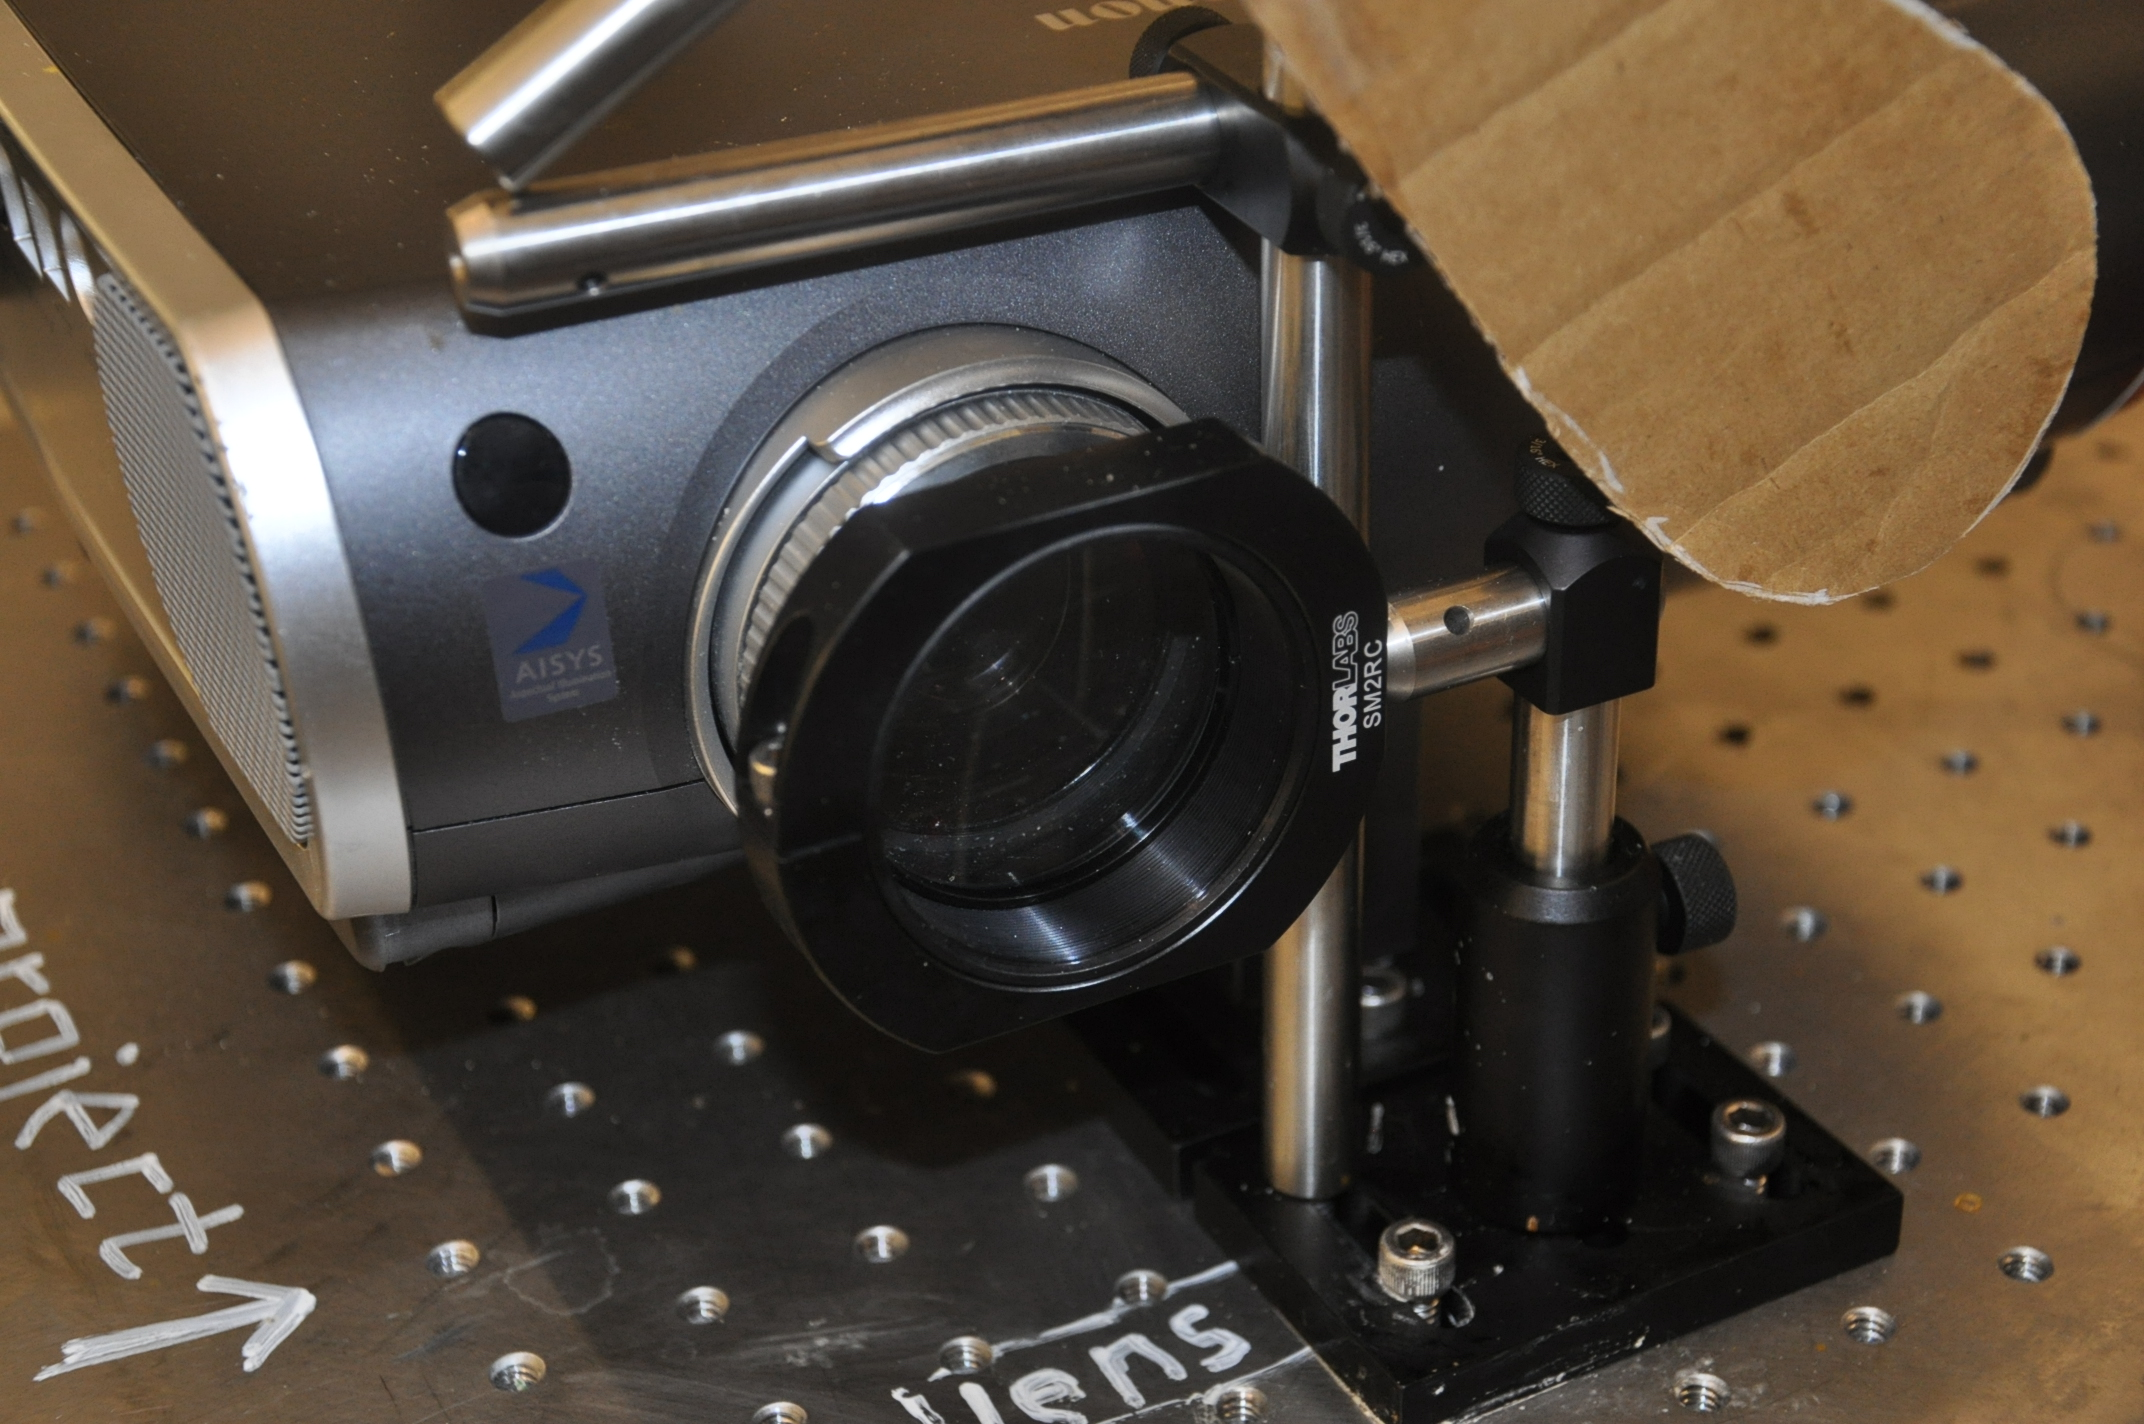
\includegraphics[width=0.33\textwidth]{intro1-1-2.jpg}} &
    The convex lens is used to decrease the projected image as well as shorten the image distance. 
    Then image is able to projected on the sample holder fix on the linear stage next to the projector. 
    A light barrier is set in front of the lens. It's used to block the optical path.
    As the convex lens is well adjusted, it's strongly adviced not to adjust it again in general use. But if 
    you have to, please see the appendix \ref{sec:convex_lens_adjustment} at the end of this manual.
\end{tabularx}
\vspace{30pt}

\subsubsection{Mirror}\label{sec:mirror}
\begin{tabularx}{\textwidth}{ cX }
    \raisebox{-0.9\height}{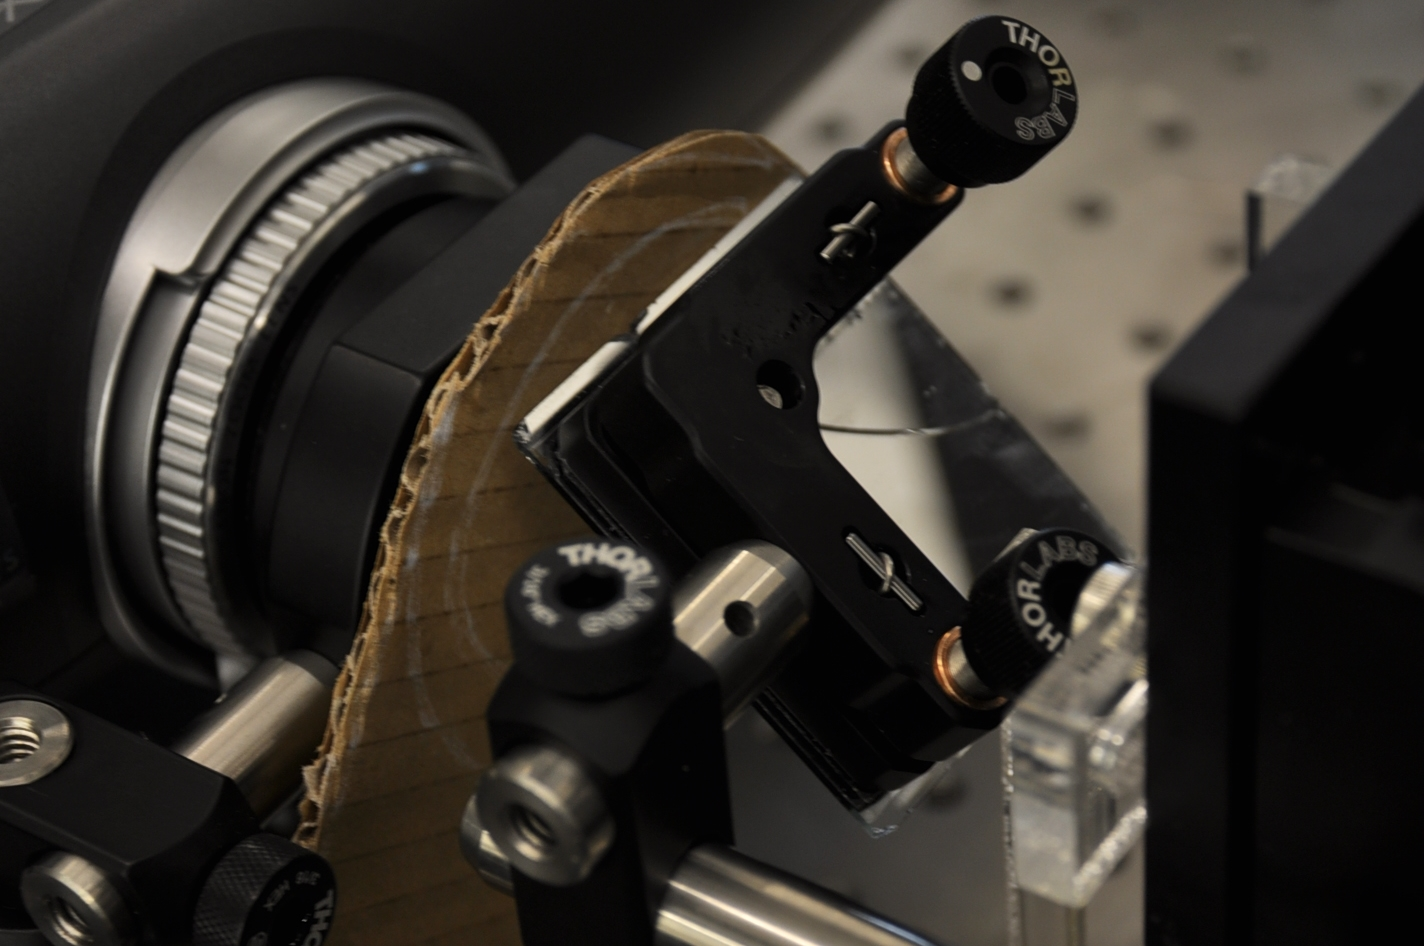
\includegraphics[width=0.33\textwidth]{intro1-1-3.jpg}} &
    The mirror rotate the main optical axis and let the image be just pojected on the sample 
    holder. Note that the mirror should be placed in a specific distance in front of the lens. More details 
    about this will be introduce in section \ref{sec:linear-stage}. If you have to adjust the mirror, please 
    see the appendix \ref{sec:mirror_adjustment}.
\end{tabularx}

\subsubsection{Linear Stage}\label{sec:linear-stage}
\begin{tabularx}{\textwidth}{ cX }
    \raisebox{-0.9\height}{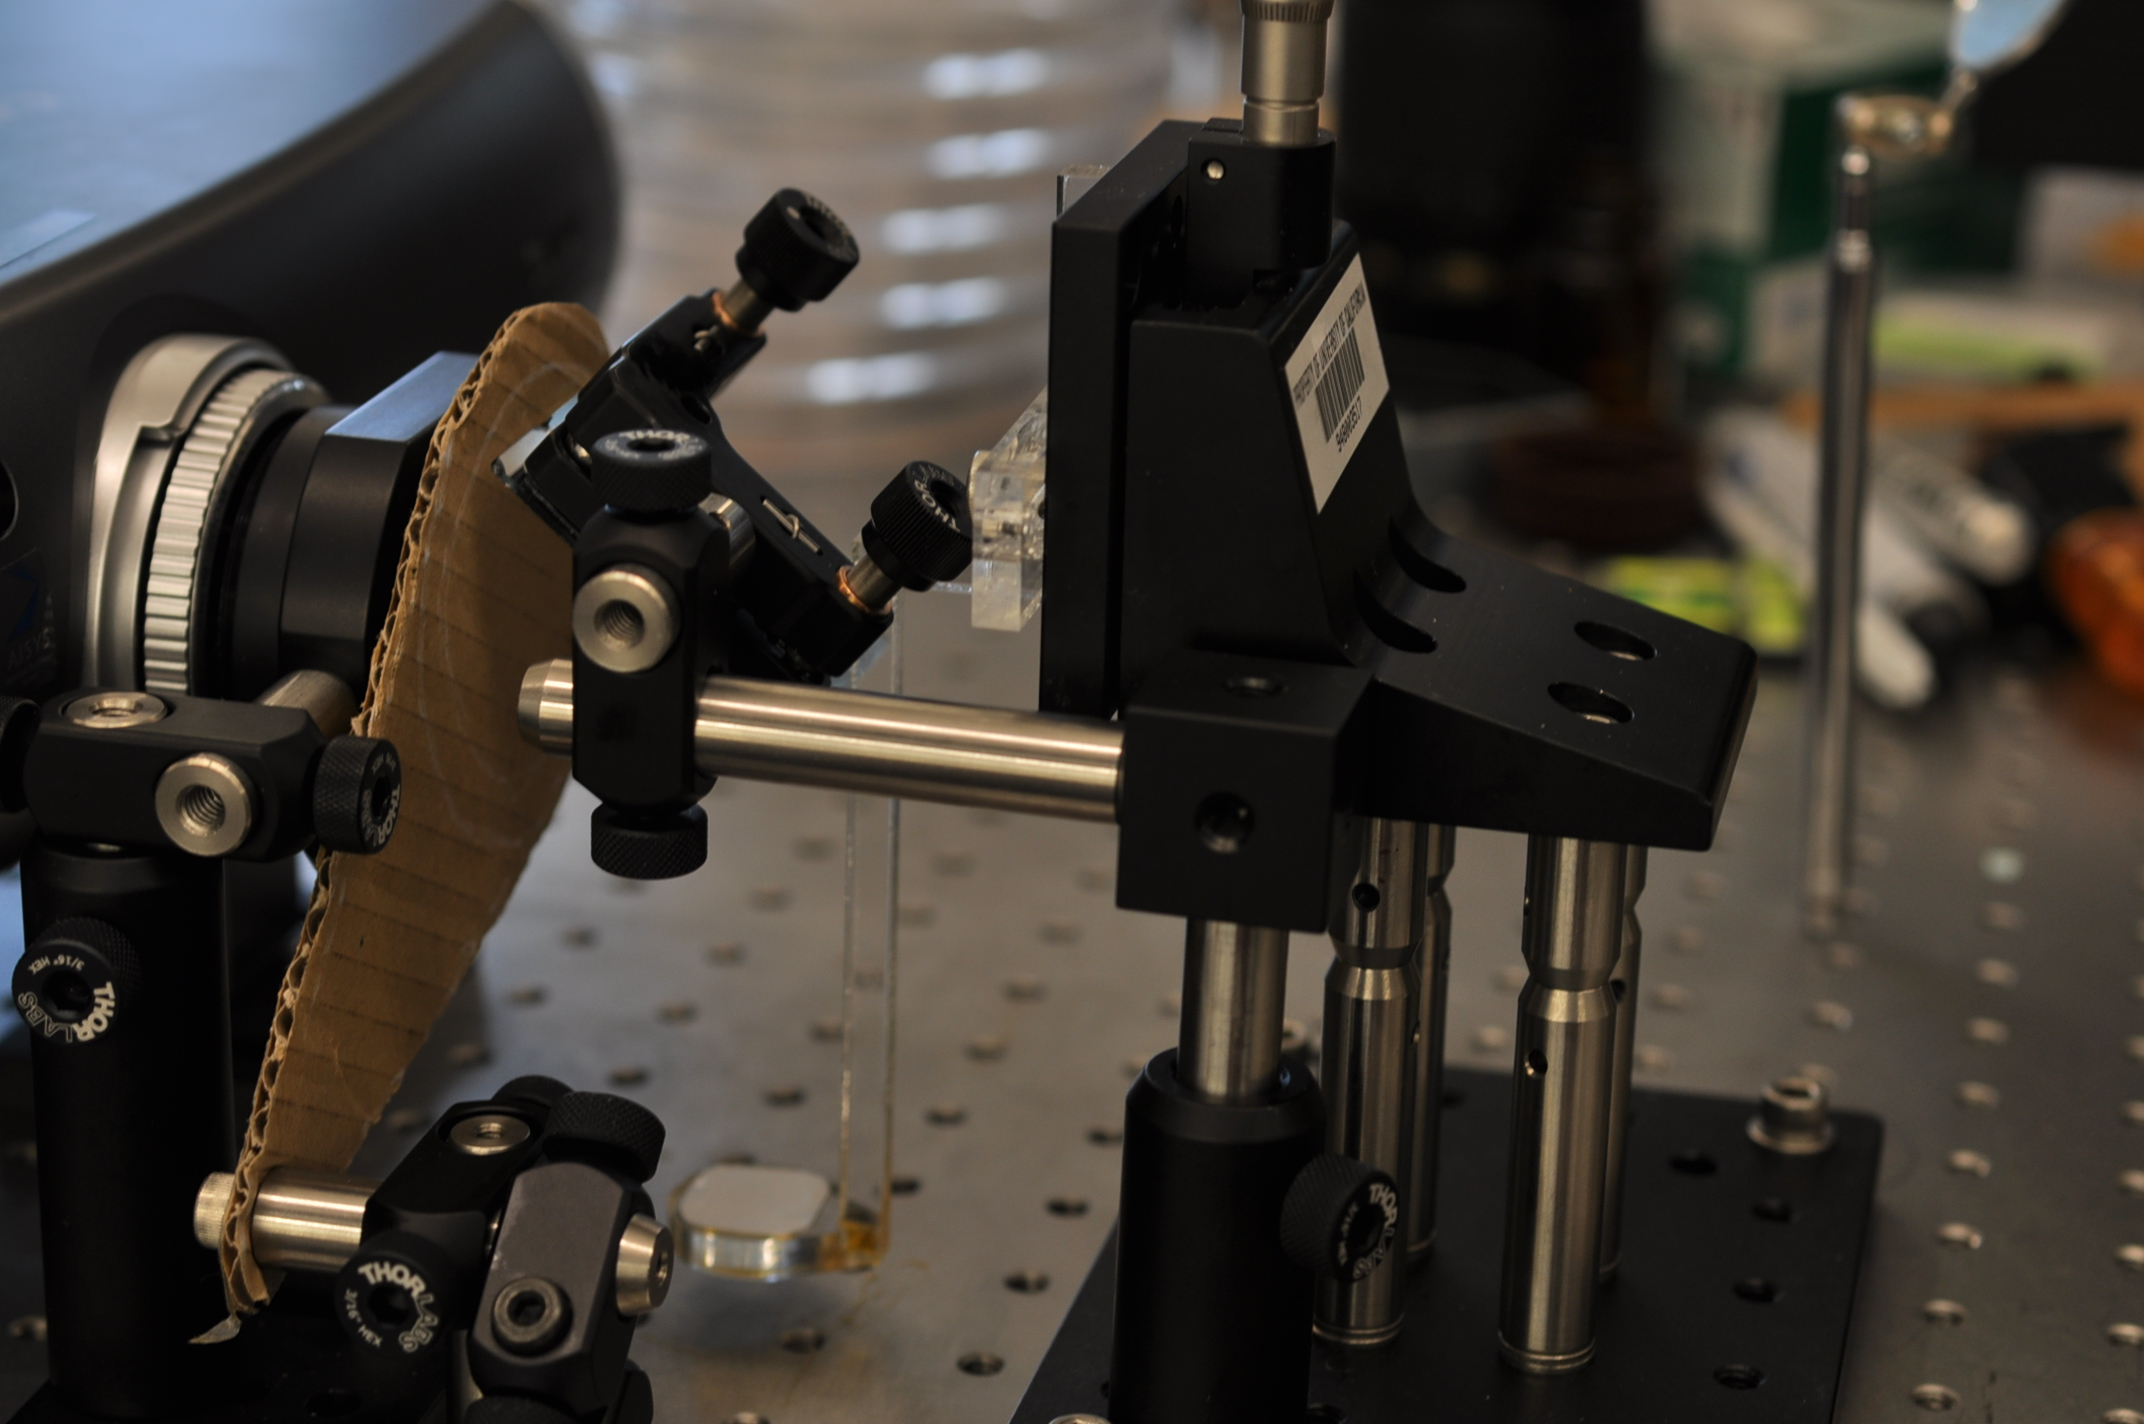
\includegraphics[width=0.33\textwidth]{intro1-1-4.jpg}} &
    The linear stage is another core part. There's a sample holder fixed on it. Rotate the knob clockwise can 
    lower the stage (as well as the sample holder) and counterclockwise upper the stage. More details about the 
    linear stage will be introduced in Appendix \ref{sec:linear_stage}. The stage is fixed on a bign base and 
    the mirror mentioned above is fixed on it too. So Let's define the \textit{stage assembly} 
    \footnote {The important words will be printed in italic font.}
    as \textit{stage} + \textit{base} + \textit{sample holder} + \textit{mirror}. 

\end{tabularx}
\vspace{10pt}

\subsection{Software}\label{sec:software}             
The portable printer actually do not need any softwares because it meant to be operated manually. But there
are still some works on computer.

When you need to \textbf{change the projecter's image output}, you should change the desktop background of the 
computer by \textbf{right click - set background}.

\begin{tabularx}{\textwidth}{ XXX }
    \raisebox{-\height}{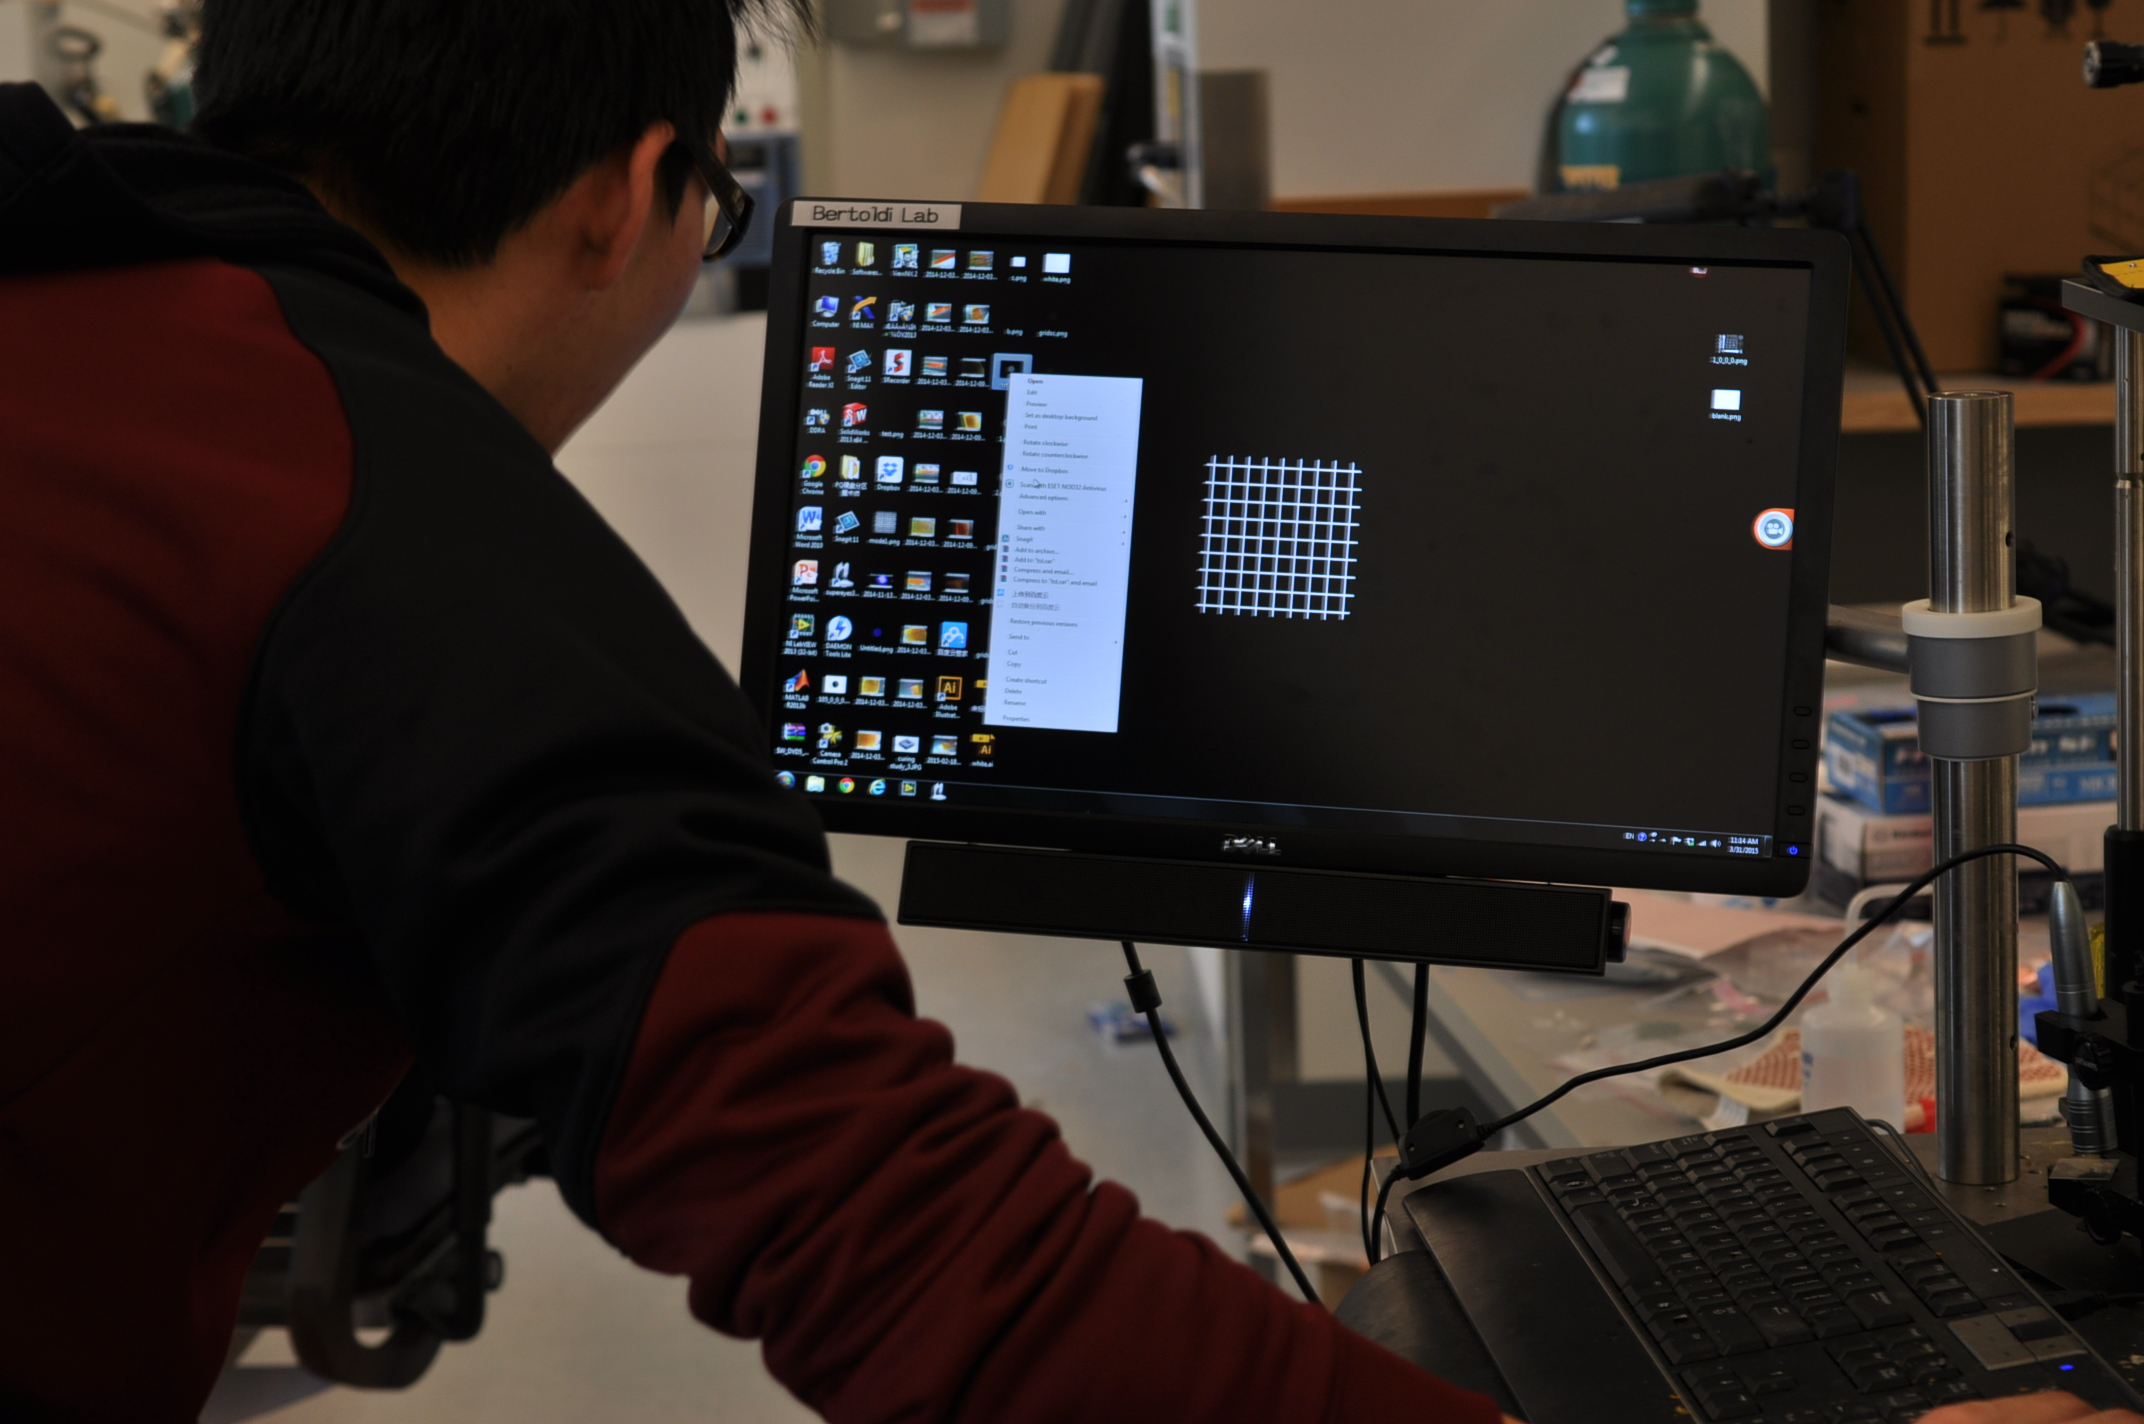
\includegraphics[width=0.3\textwidth]{software1_2.jpg}}
    &\raisebox{-\height}{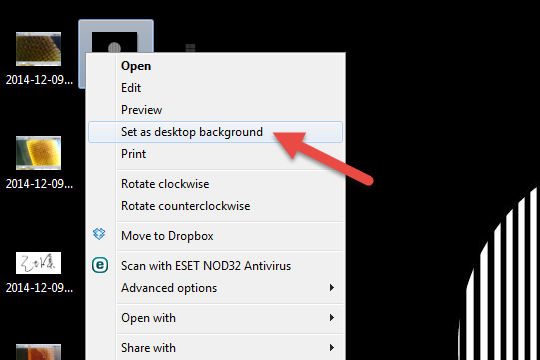
\includegraphics[width=0.3\textwidth]{software1_1.png}}
    &\raisebox{-\height}{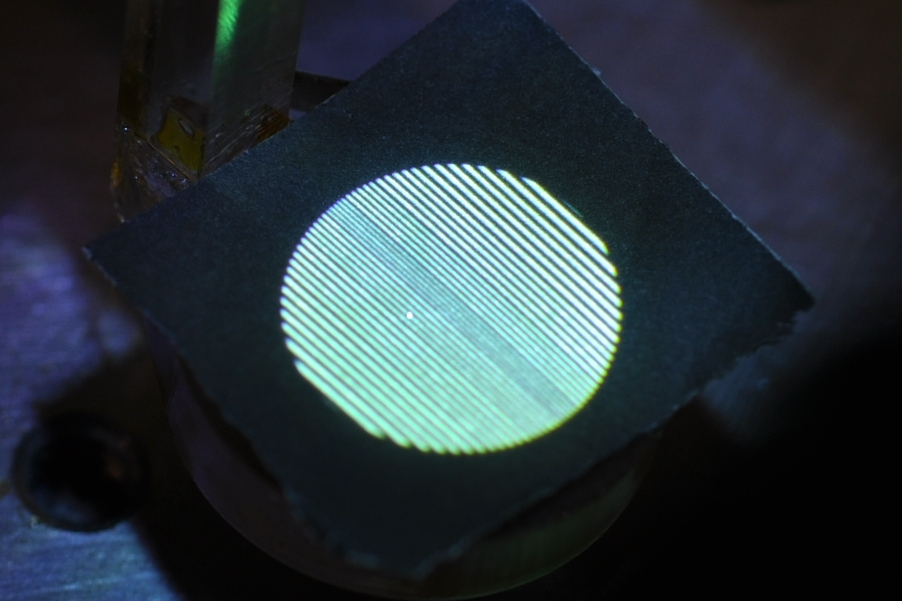
\includegraphics[width=0.3\textwidth]{pre4r.jpg}}\\
    \\
\end{tabularx}


\textbf{An python program is written to help with the operation}. It can give out vocal instructions to assist 
you to do the right action at the right time. Five parameters should be set everytime you open the program.
\begin{itemize}   
    \item Number of layers : It depends on the height of sample and the thickness of each layer. 
    \item \textit{Thickness of each layer ($\mu$m)} : The thickness of each layer determines the resolution on Z-axis. 
        The smaller it is, the higher Z-axis' resolution is.
    \item \textit{Curing time of each layer (s)} : It depends on the layer thickness and the material you use. You 
        should know the material well and test it before printing. As PEG/PEGDA system with 2wt\% Photo-initiator, 
        20 seconds are recomanded and with the thickness of each layer increasing the curing time should grow up too.
    \item \textit{Curing time of firest layer (s)} : First layer is a bit different. The curing time should be set longer 
        than other layers to make sure the sample can be bonded well with the sample holder. This is always set to twice 
        or three times of other layers' curing time.
    \item \textit{Fluid flowing time (s)} : It also depends on what kind of materials you use. When one layer is printed, 
        the sampler holder will move down for next layer and this parameter is set to let the program know how long it 
        should wait for the material flowing over the whole sample. Actually in the program, the sample holder will move 
        down three times of the layer thickness first, wating for flowing time, then move up twice of layer thickness and 
        wait  for flowing time angin. In this way the flowing progress will be speeded up. 30 seconds are recommanded for 
        PEG/PEGDA system.
\end{itemize}
After you finishing inputing the parameters, the vocal assistance will start in 10 seconds.             


\begin{tabularx}{\textwidth}{ XXX }
    \raisebox{-\height}{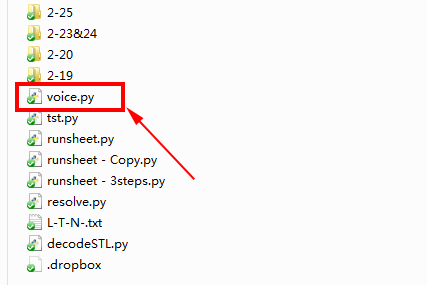
\includegraphics[width=0.3\textwidth]{voice_folder.png}}
    &\raisebox{-\height}{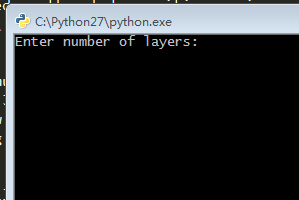
\includegraphics[width=0.3\textwidth]{voice_interface.png}}
    &\raisebox{-\height}{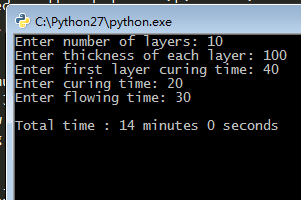
\includegraphics[width=0.3\textwidth]{voice_interface2.png}}\\
    \\
\end{tabularx}



\subsection{Materials}\label{sec:materials}
See \textit{Operation manual for P$\mu$SL 3D-Printer in precision mode} for more details about the materials.
\vspace{20pt}


\section{Normal Operation Procedure}\label{sec:page-layout}
In this section, I will introduce the normal operation precedure for the 3d-printer. Just follow the steps. \\
\textbf {To your own safety, always wear gloves before doing anything and wash hands after experiments.}

\subsection{Preperation}\label{sec:preperation}

\begin{itemize}
        \begin{tabularx}{\textwidth}{ XXX }
        \item \textbf{Step 1} : Put the stage in right place. The mirror shall be about $\sim\frac{1}{2}$ inch 
            in front of the lens. Also make sure that the screws on corners are embedded into the holes on the table.
            &\raisebox{-\height}{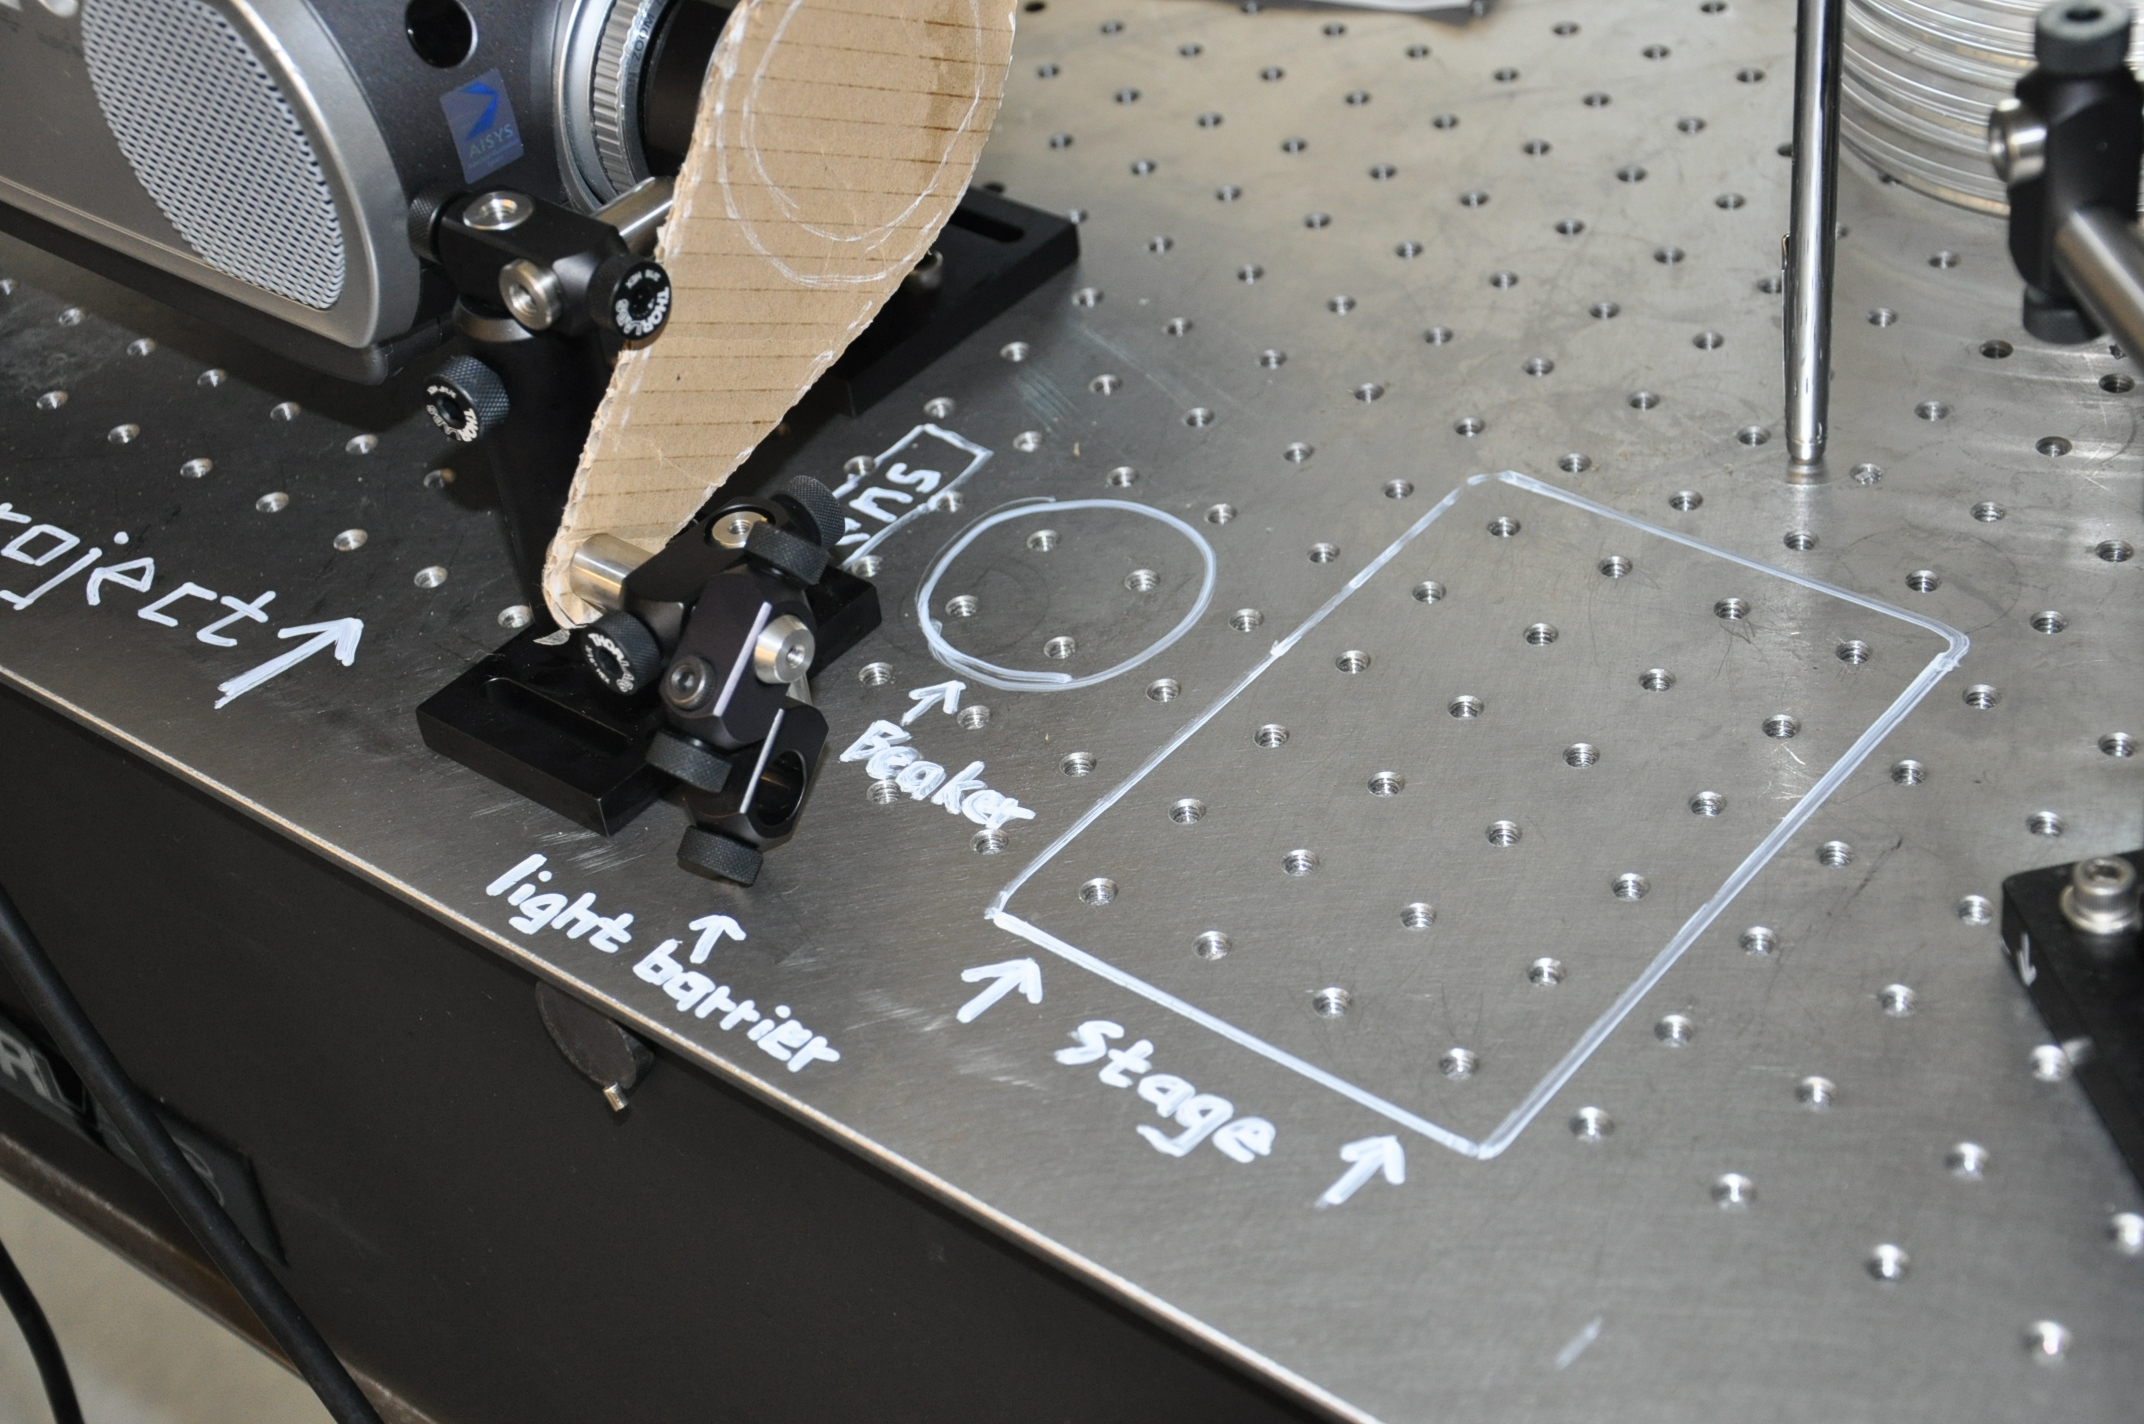
\includegraphics[width=0.3\textwidth]{pre2l.jpg}}
            &\raisebox{-\height}{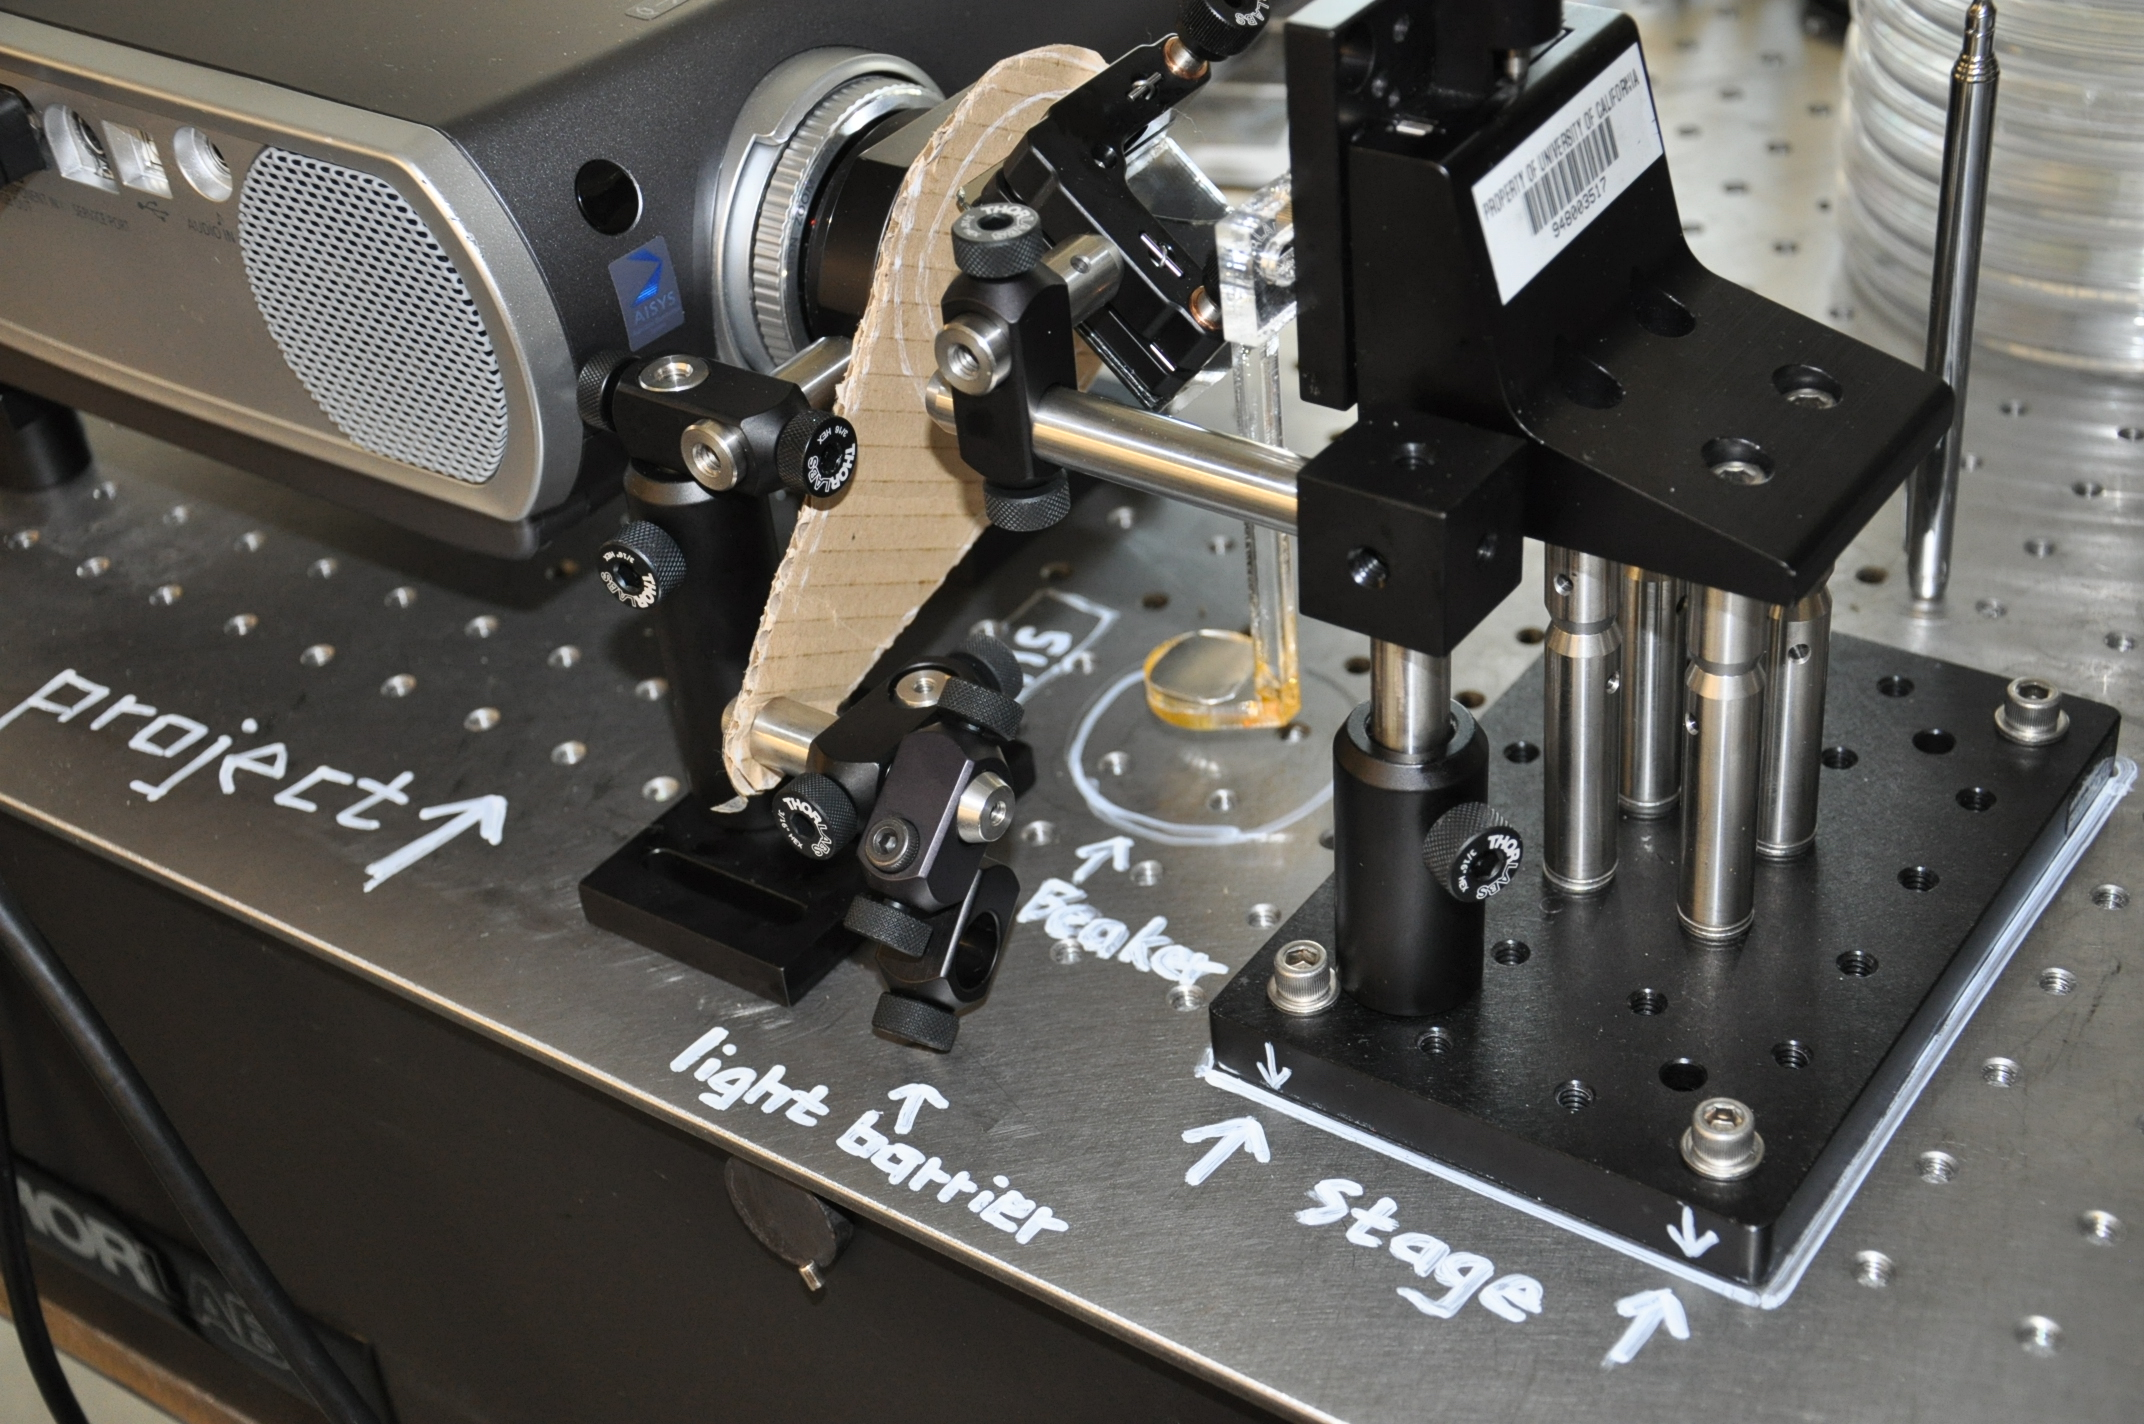
\includegraphics[width=0.3\textwidth]{pre2r.jpg}}\\
            \\
        \end{tabularx}

        \begin{tabularx}{\textwidth}{ XXX }
        \item \textbf{Step 2} : Check the position of linear stage. Make sure that the inital position is 5mm 
            as shown in picture.
            &\raisebox{-\height}{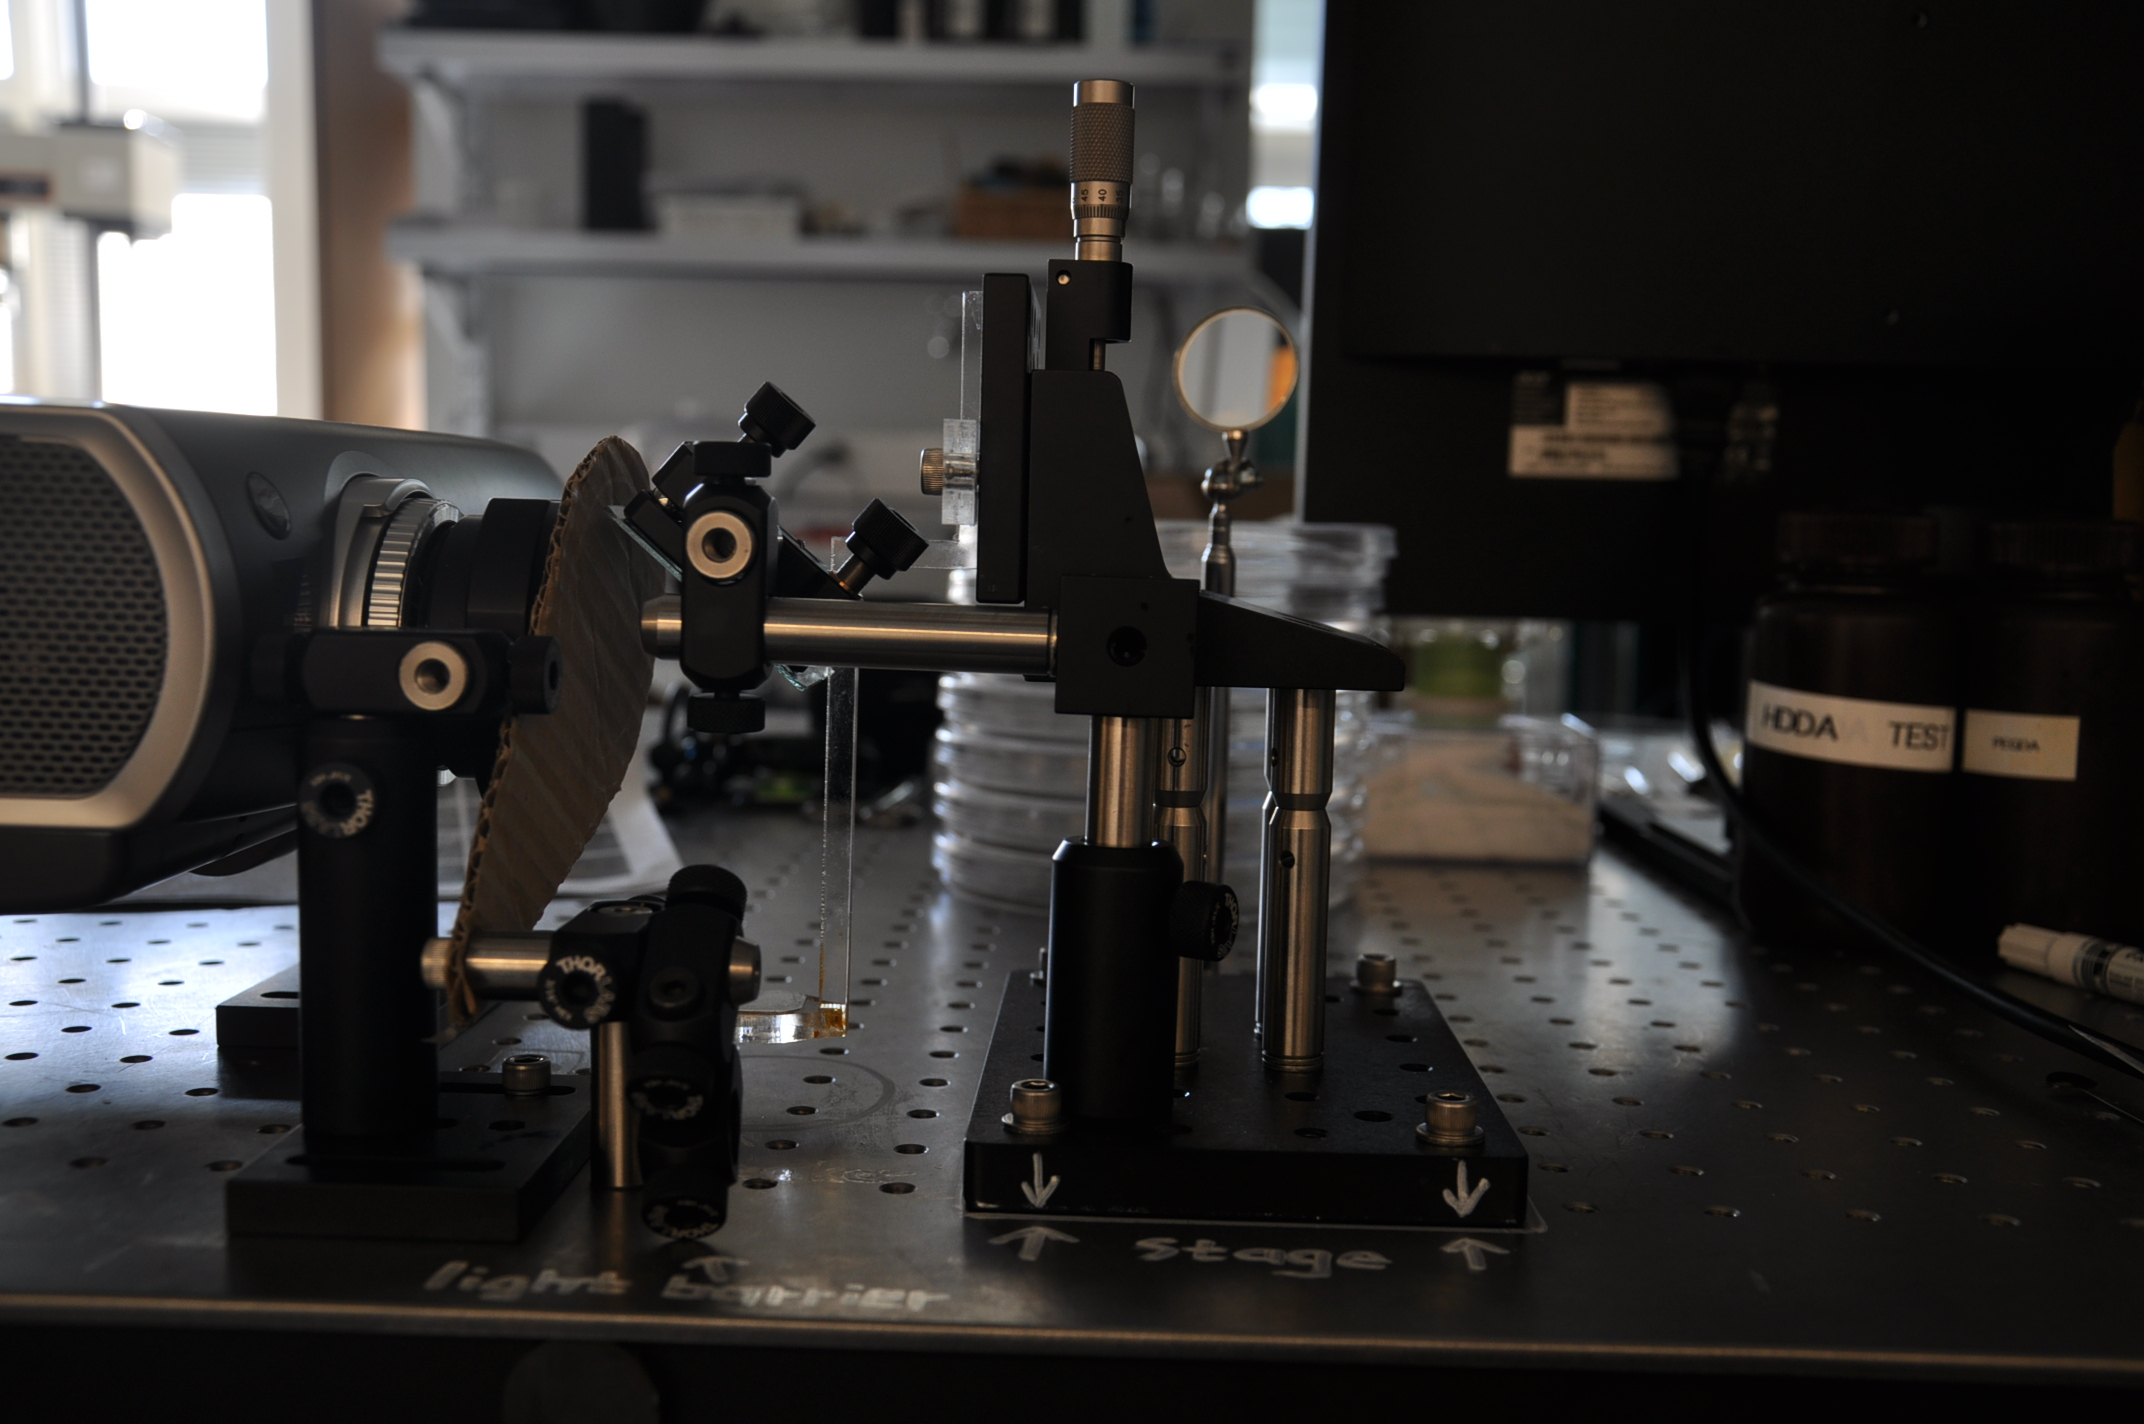
\includegraphics[width=0.3\textwidth]{pre1l.jpg}}
            &\raisebox{-\height}{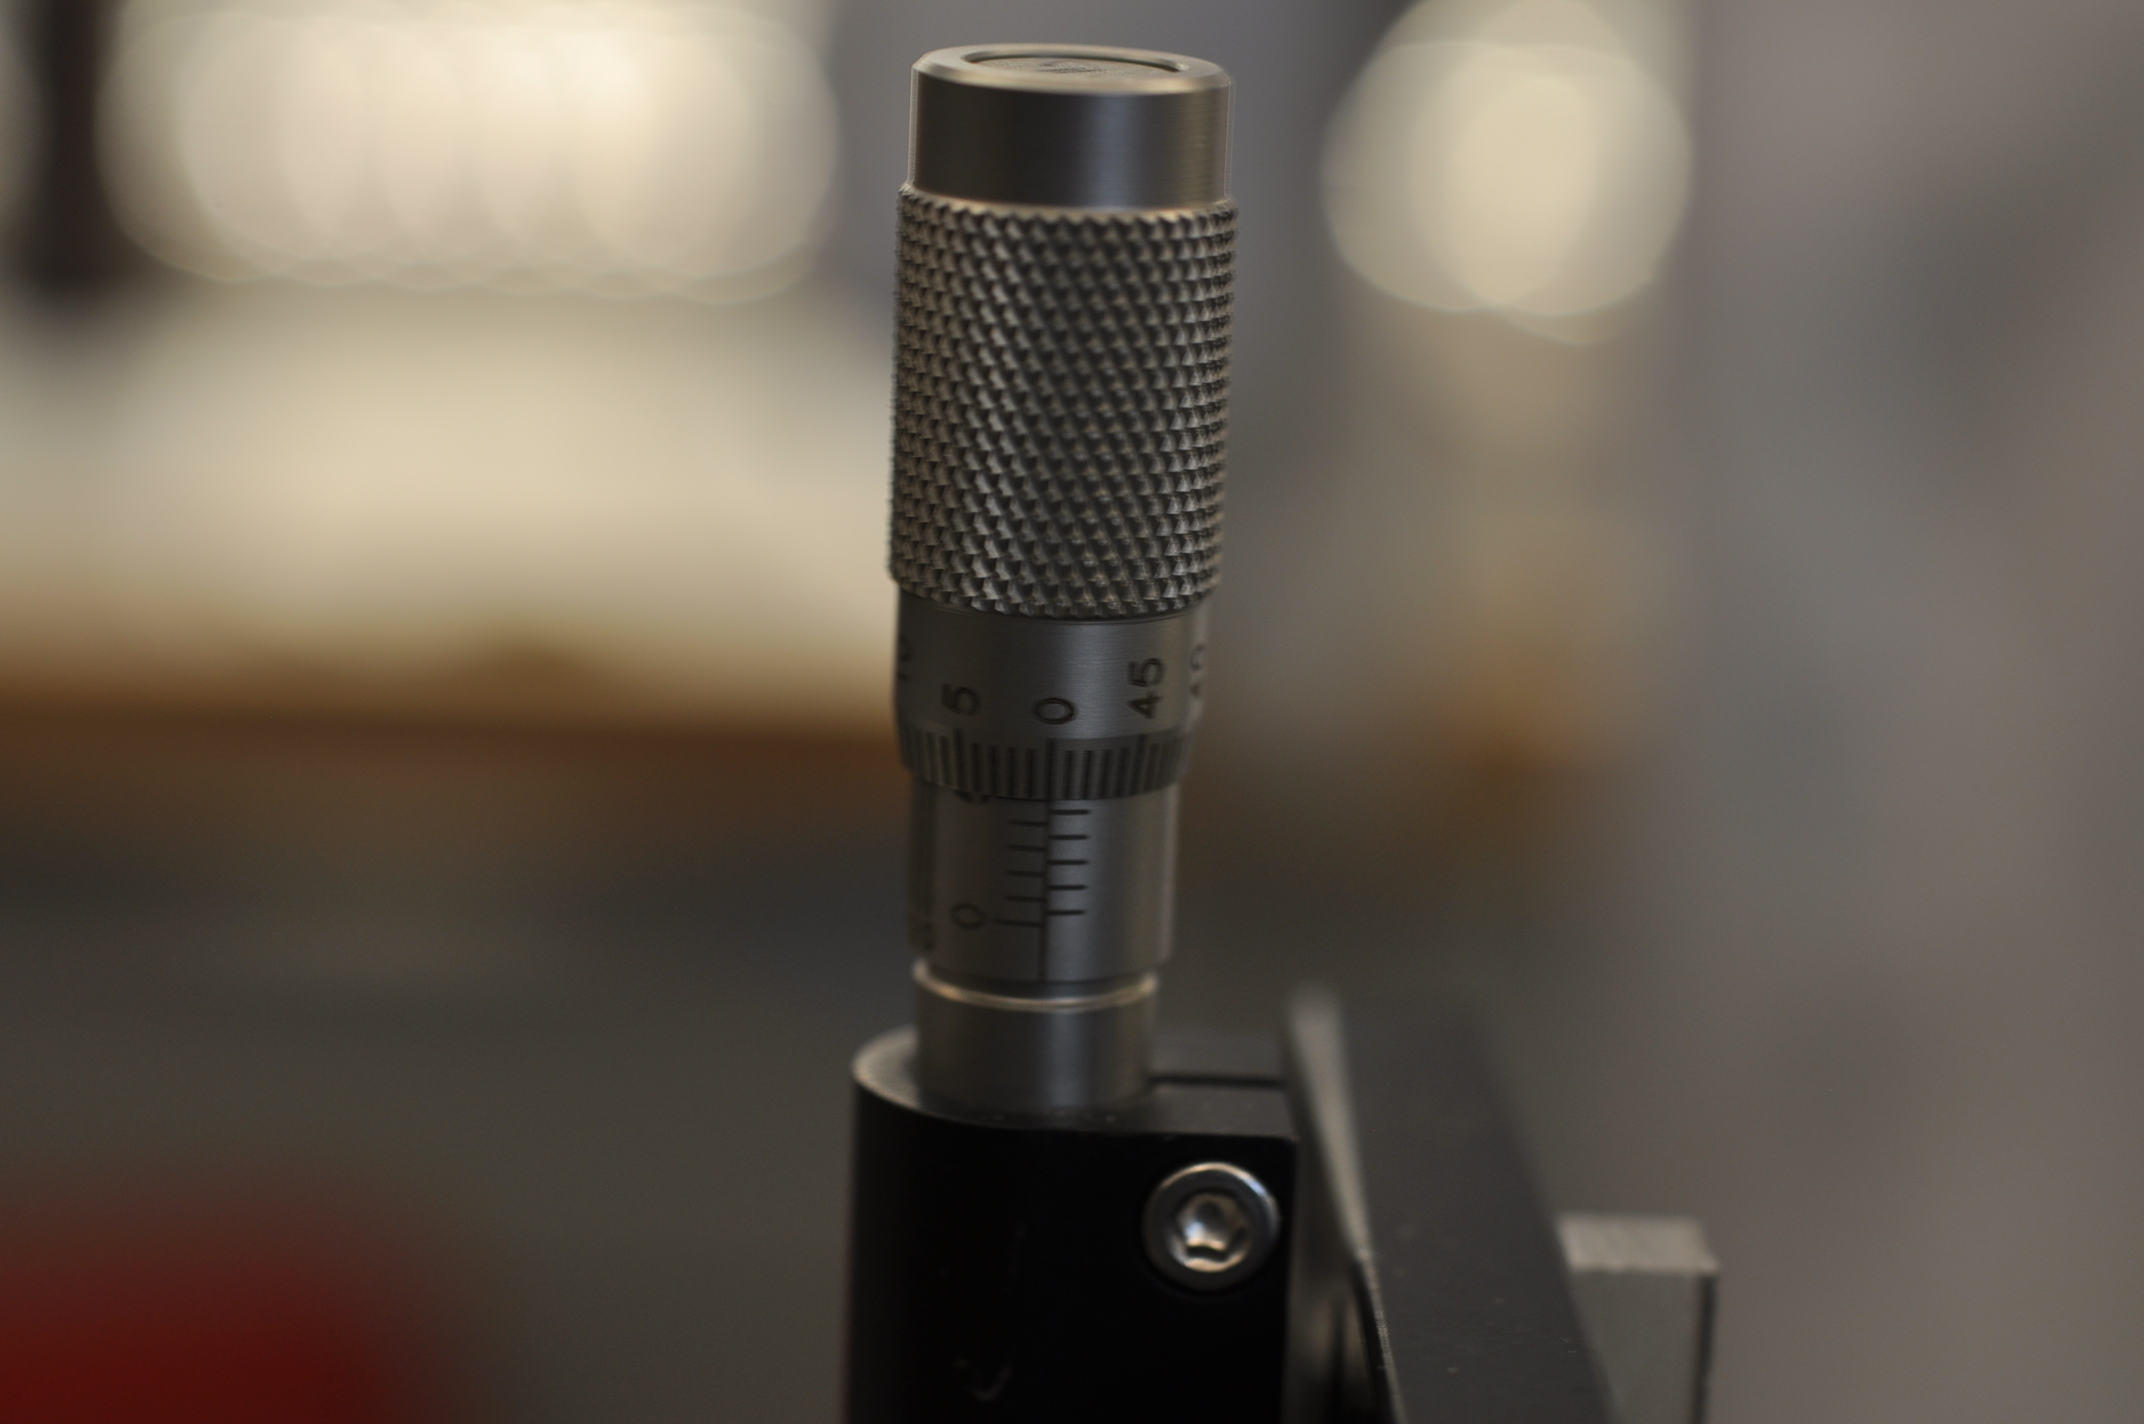
\includegraphics[width=0.3\textwidth]{pre1r.jpg}}\\
            \\
        \end{tabularx}

        \begin{tabularx}{\textwidth}{ XXX }
        \item \textbf{Step 3} : Now \textbf{open} the computer. \textbf{Set} 'tst.png' as desktop background. \textbf{Turn on} 
            the projector and \textbf{open} the light barrier by rotating it.
            &\raisebox{-\height}{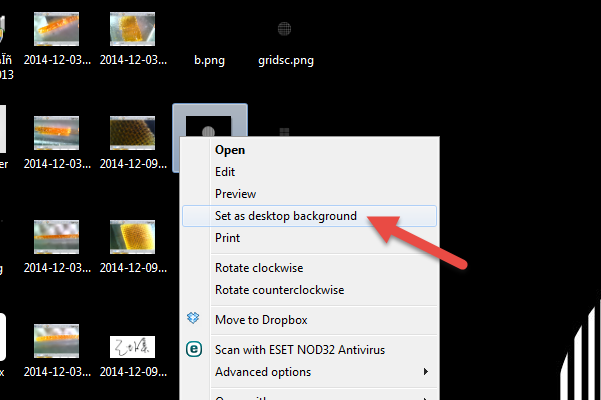
\includegraphics[width=0.3\textwidth]{pre3r.png}}
            &\raisebox{-\height}{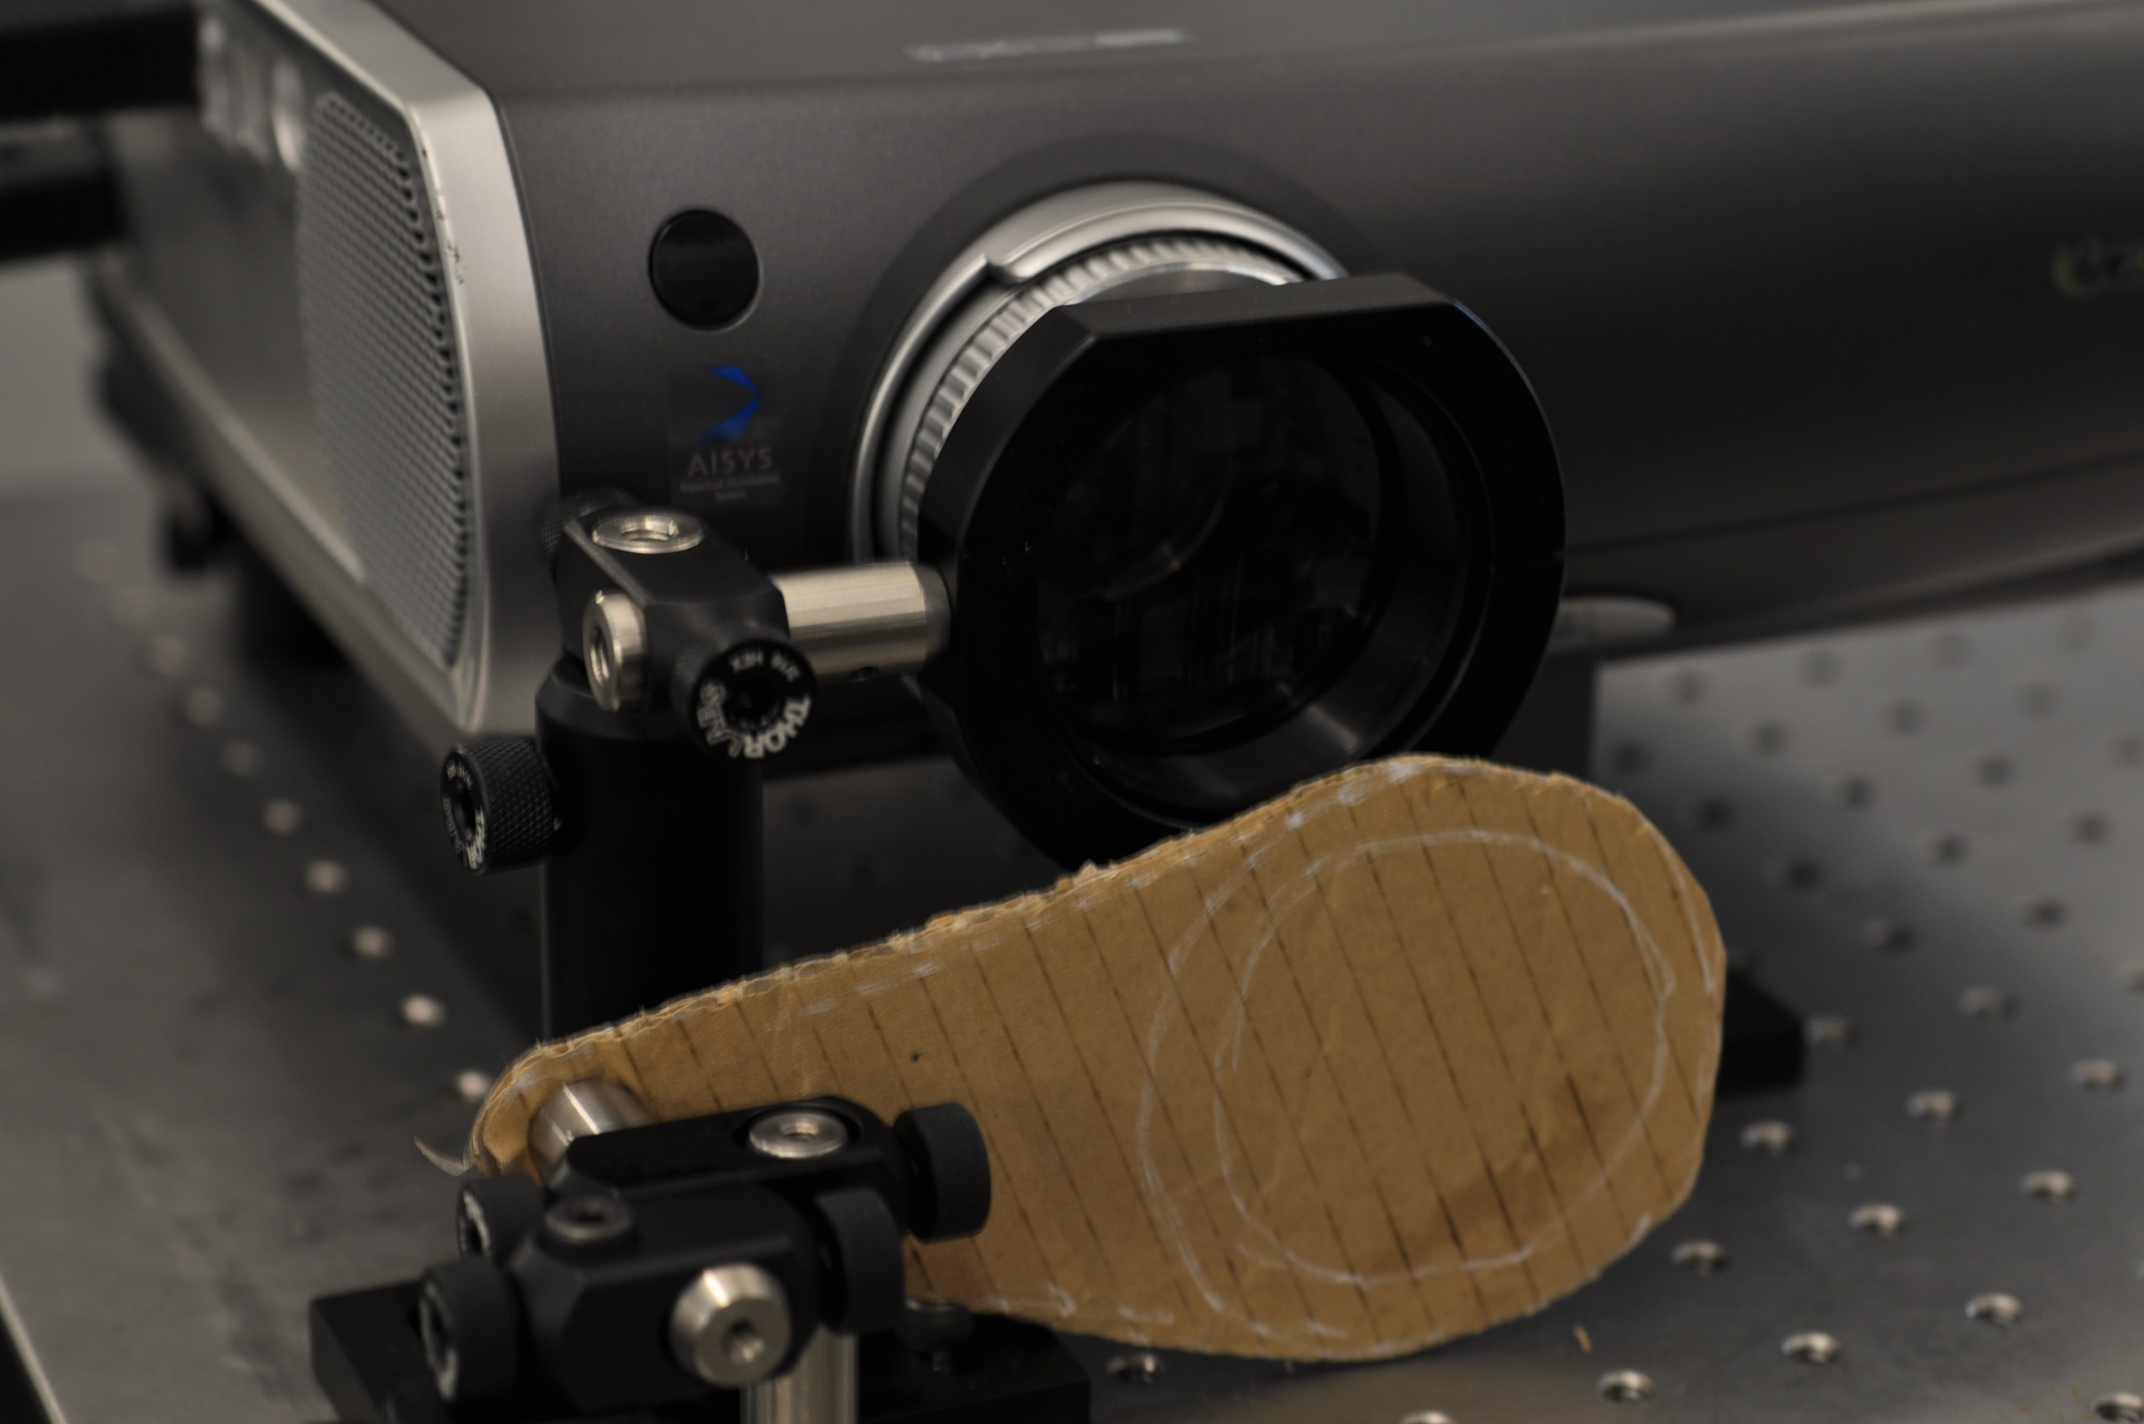
\includegraphics[width=0.3\textwidth]{pre3l.jpg}}\\
            \\
        \end{tabularx}

        \begin{tabularx}{\textwidth}{ XXX }
        \item \textbf{Step 4} : \textbf{Put} a small piece of black paper on sample holder. \textbf{Ajust} the focal length by 
            rotating the ring shown in picture until the image is sharp enough.
            &\raisebox{-\height}{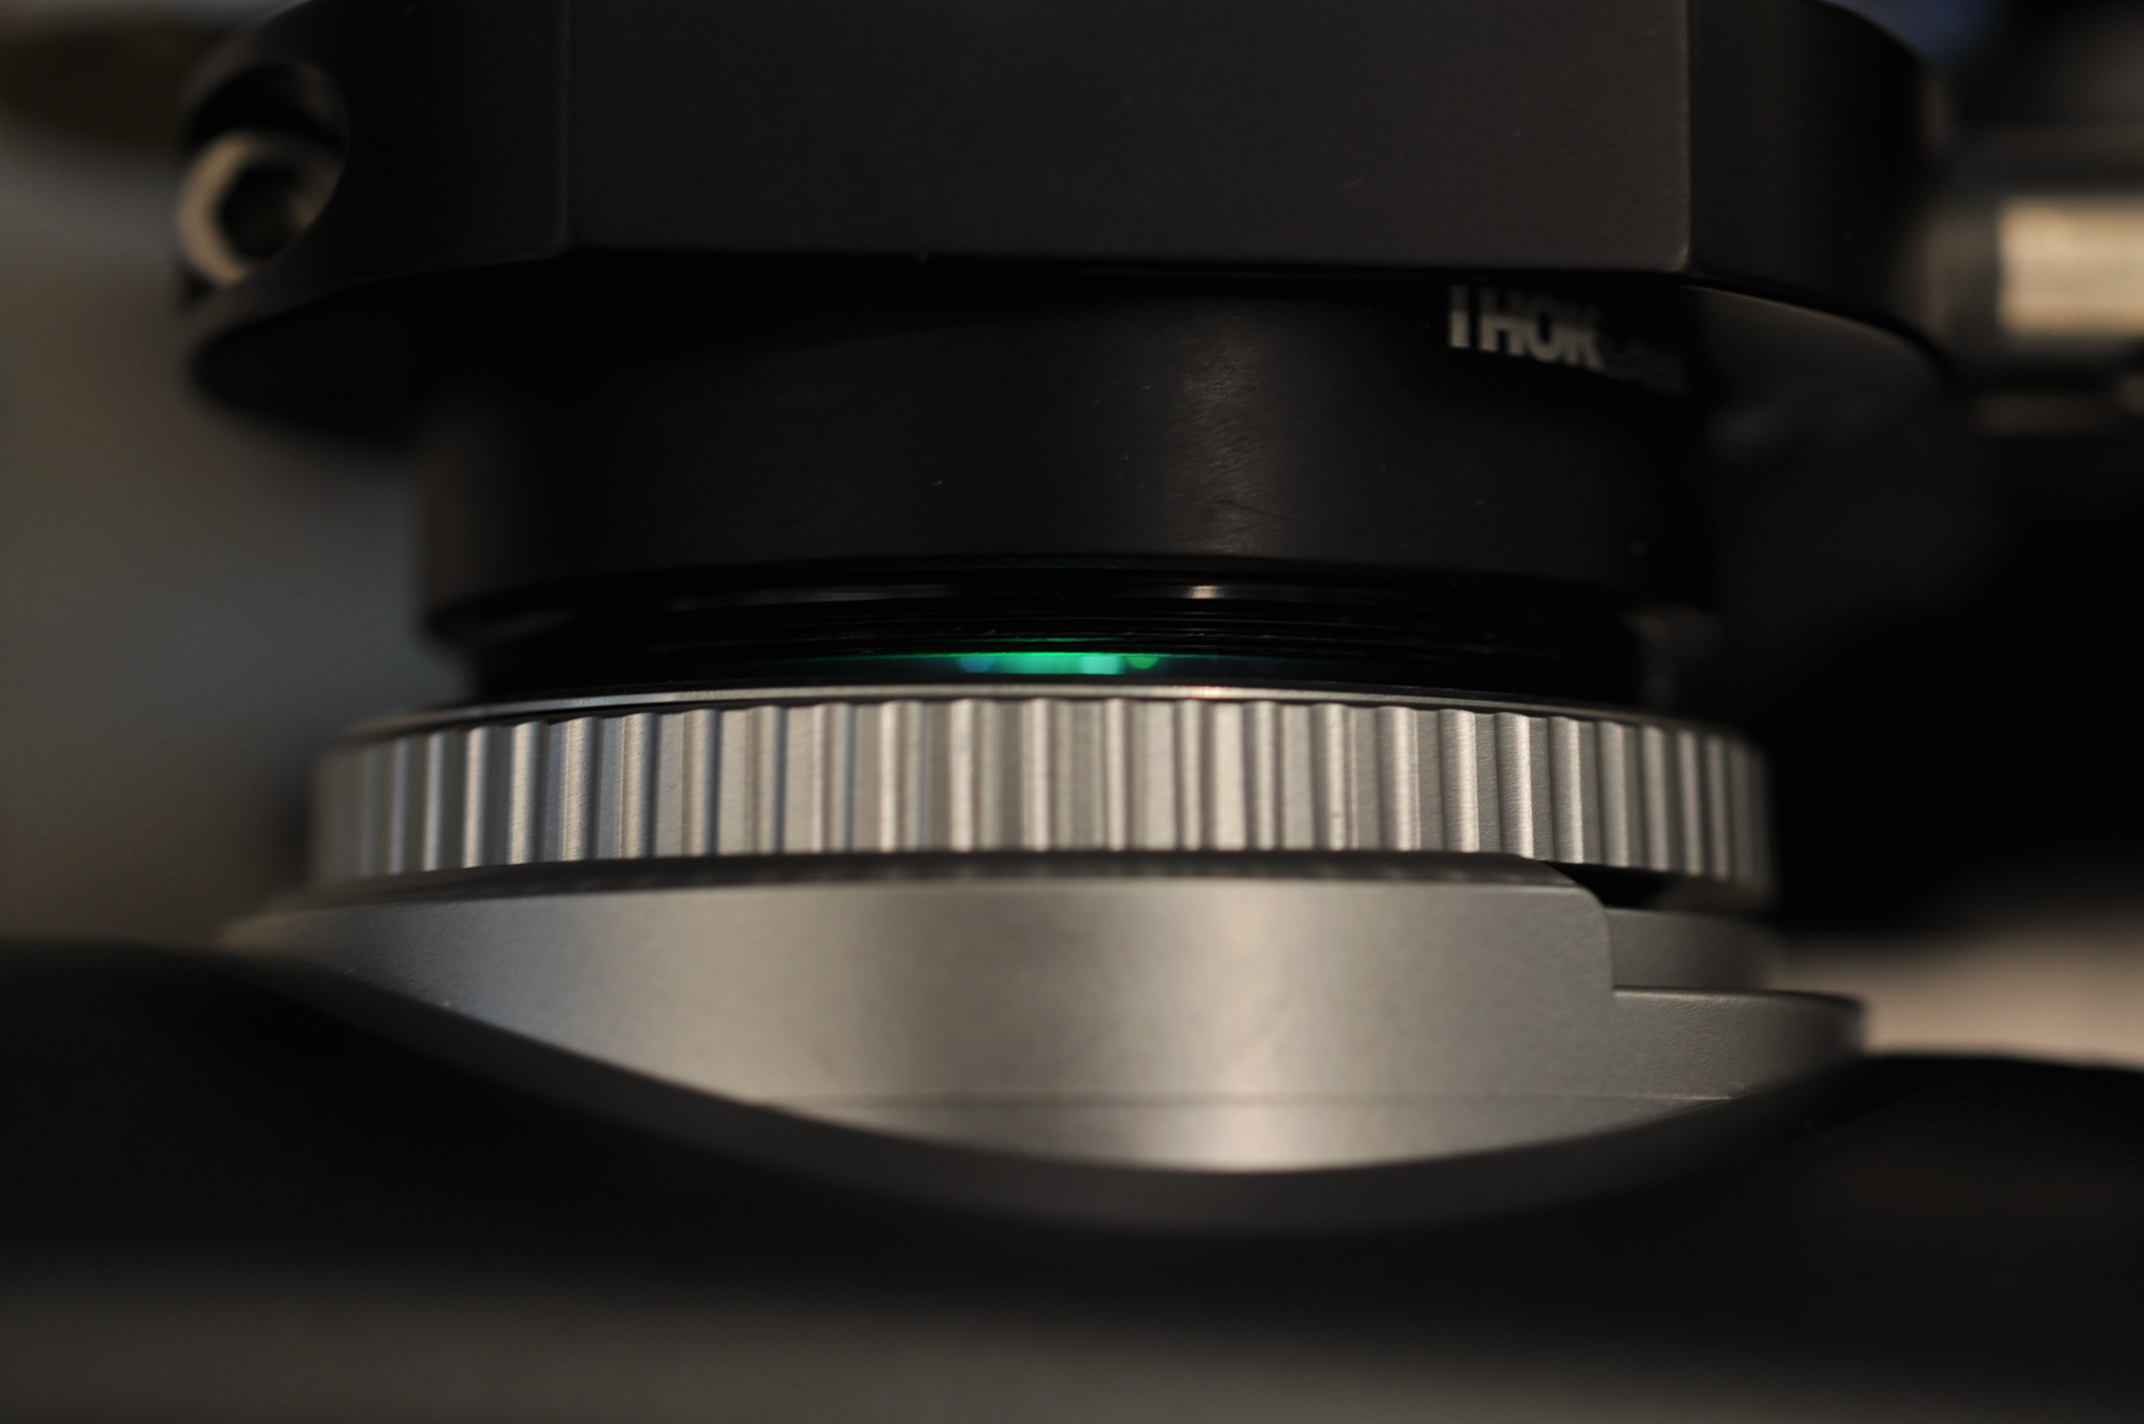
\includegraphics[width=0.3\textwidth]{pre4l.jpg}}
            &\raisebox{-\height}{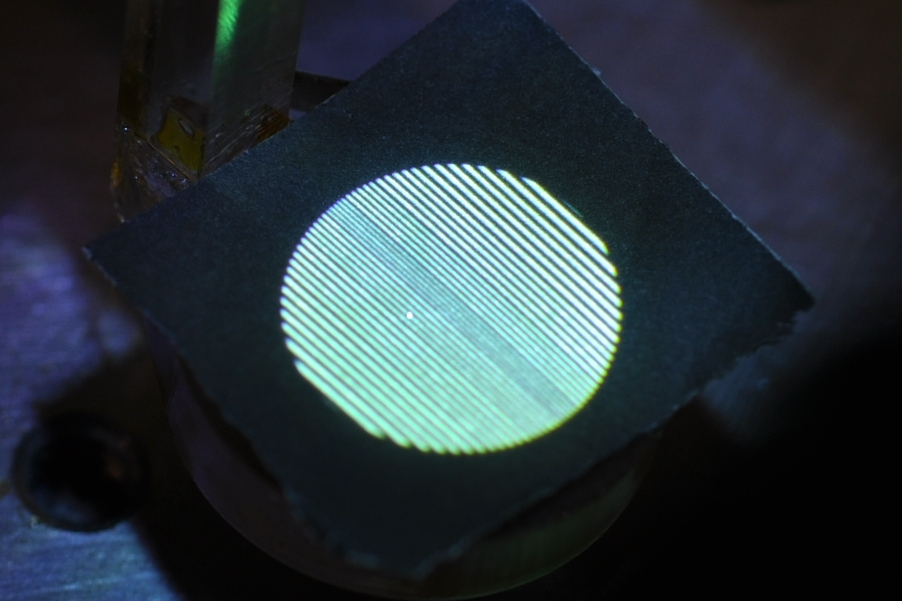
\includegraphics[width=0.3\textwidth]{pre4r.jpg}}\\
        \end{tabularx}

        \begin{tabularx}{\textwidth}{ XXX }
        \item \textbf{Step 5} : \textbf{Remove} the black paper and \textbf{close} the light barrier, now the device is ready for printing.
            \\
        \end{tabularx}
\end{itemize}

\vspace{10pt}
\subsection{Printing}\label{sec:printing}

\begin{itemize}
        \begin{tabularx}{\textwidth}{ XXX }
        \item \textbf{Step 1} : \textbf{Add} about 20ml of material into a beaker outside. Take away the stage assembly so that the 
            beaker can be put on the marker. Then put the stage assembly back carefully on the marker on table.
            &\raisebox{-0.95\height}{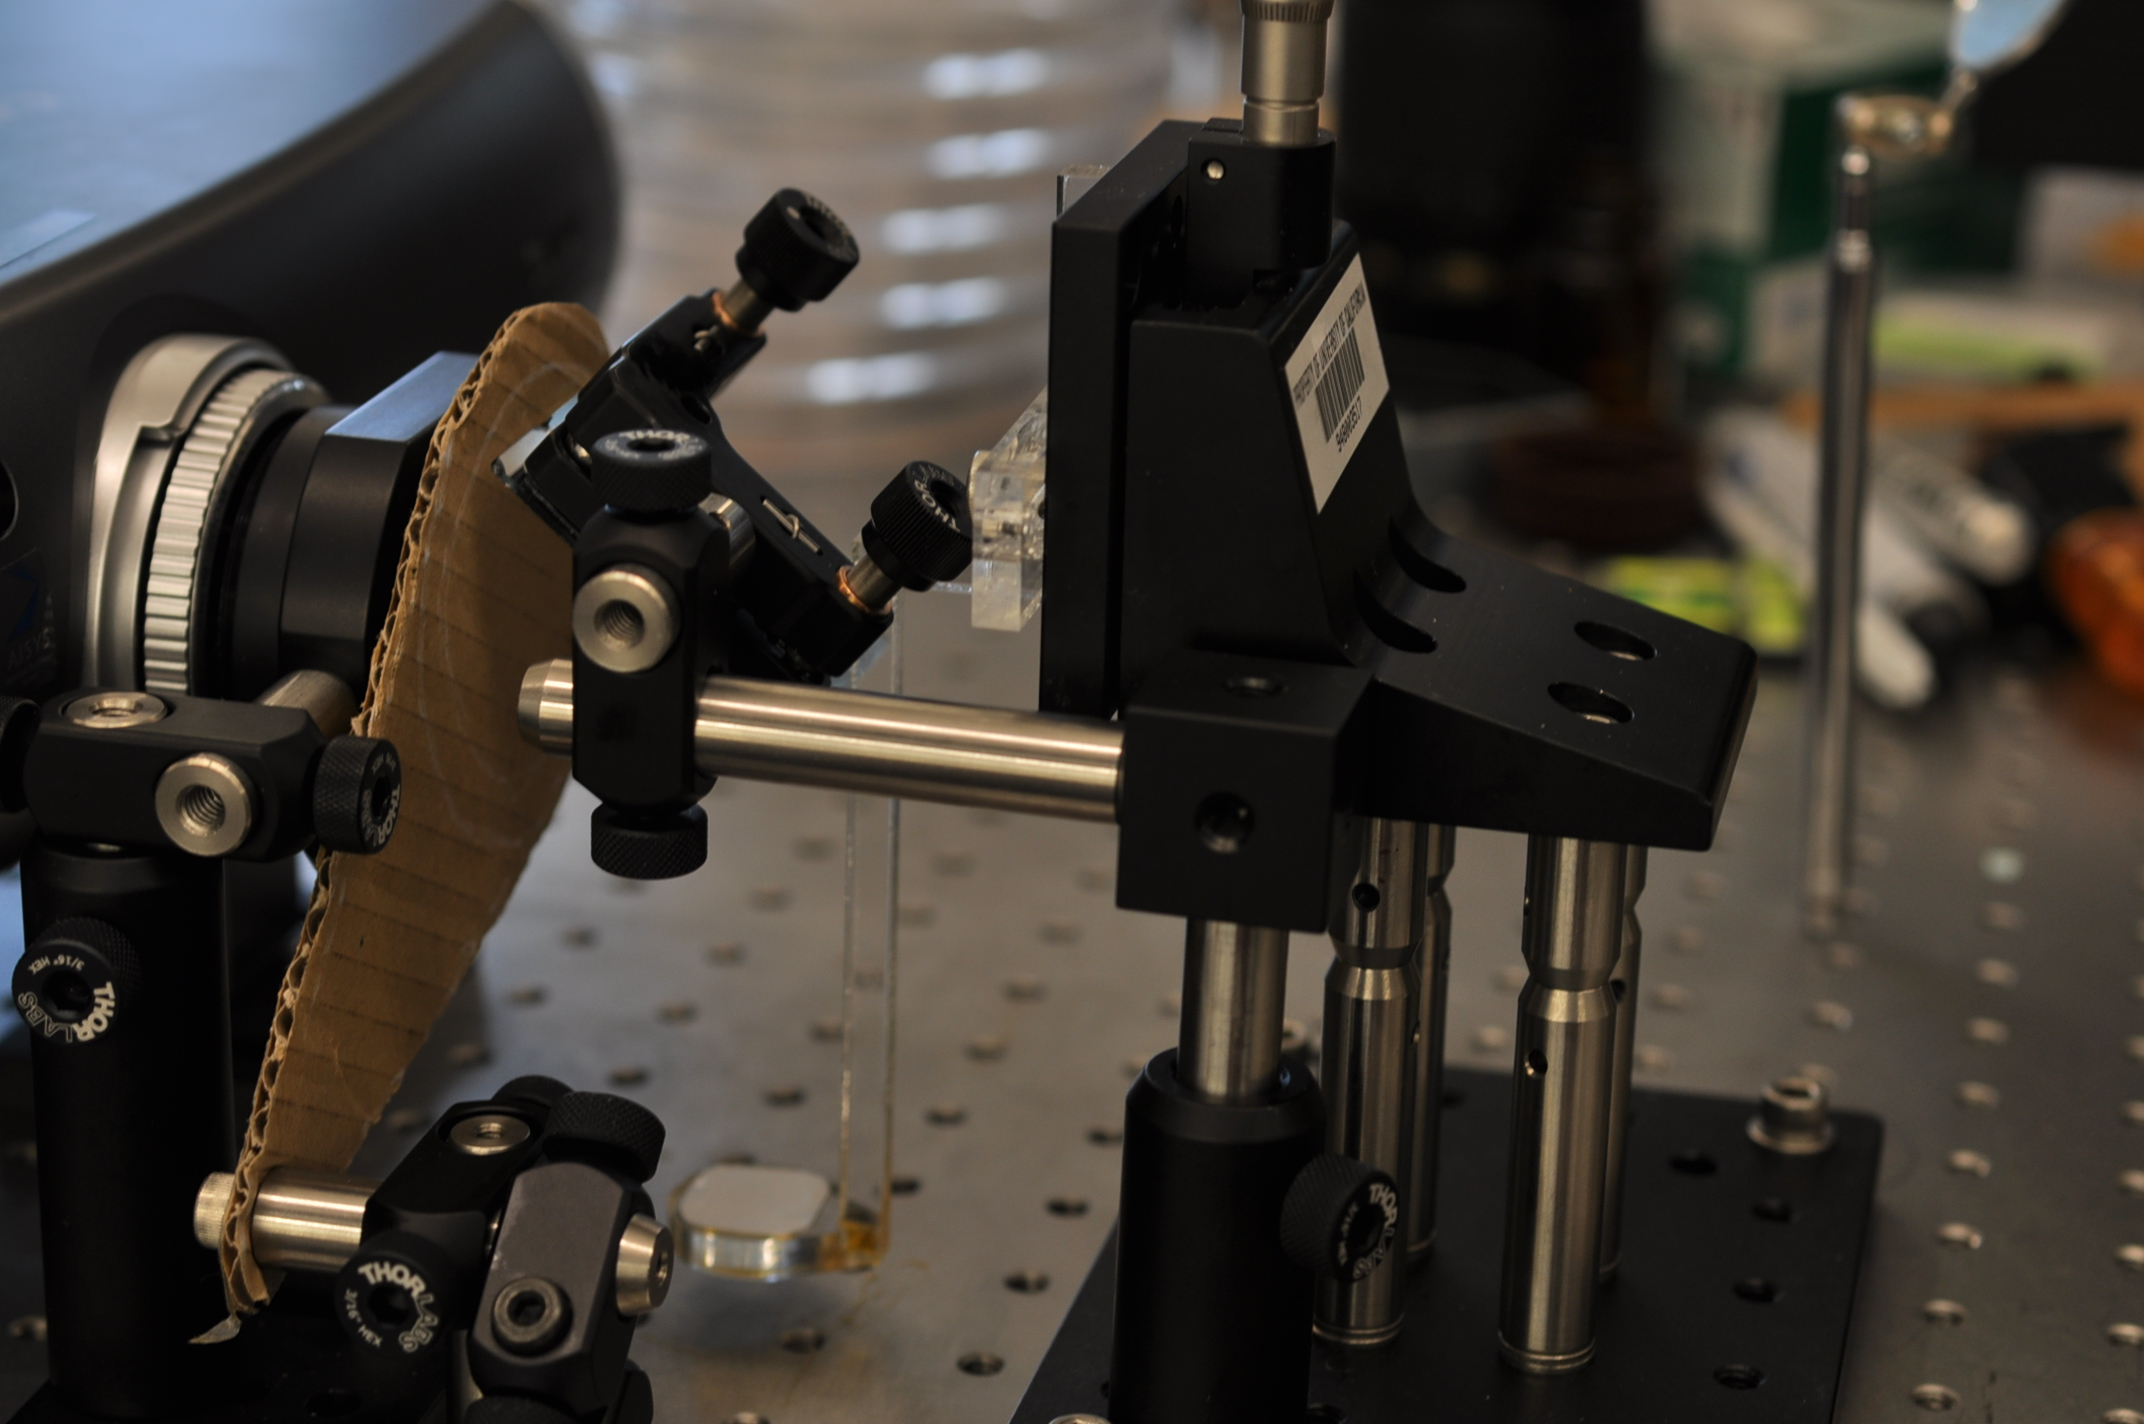
\includegraphics[width=0.3\textwidth]{pre5l.jpg}}
            &\raisebox{-0.95\height}{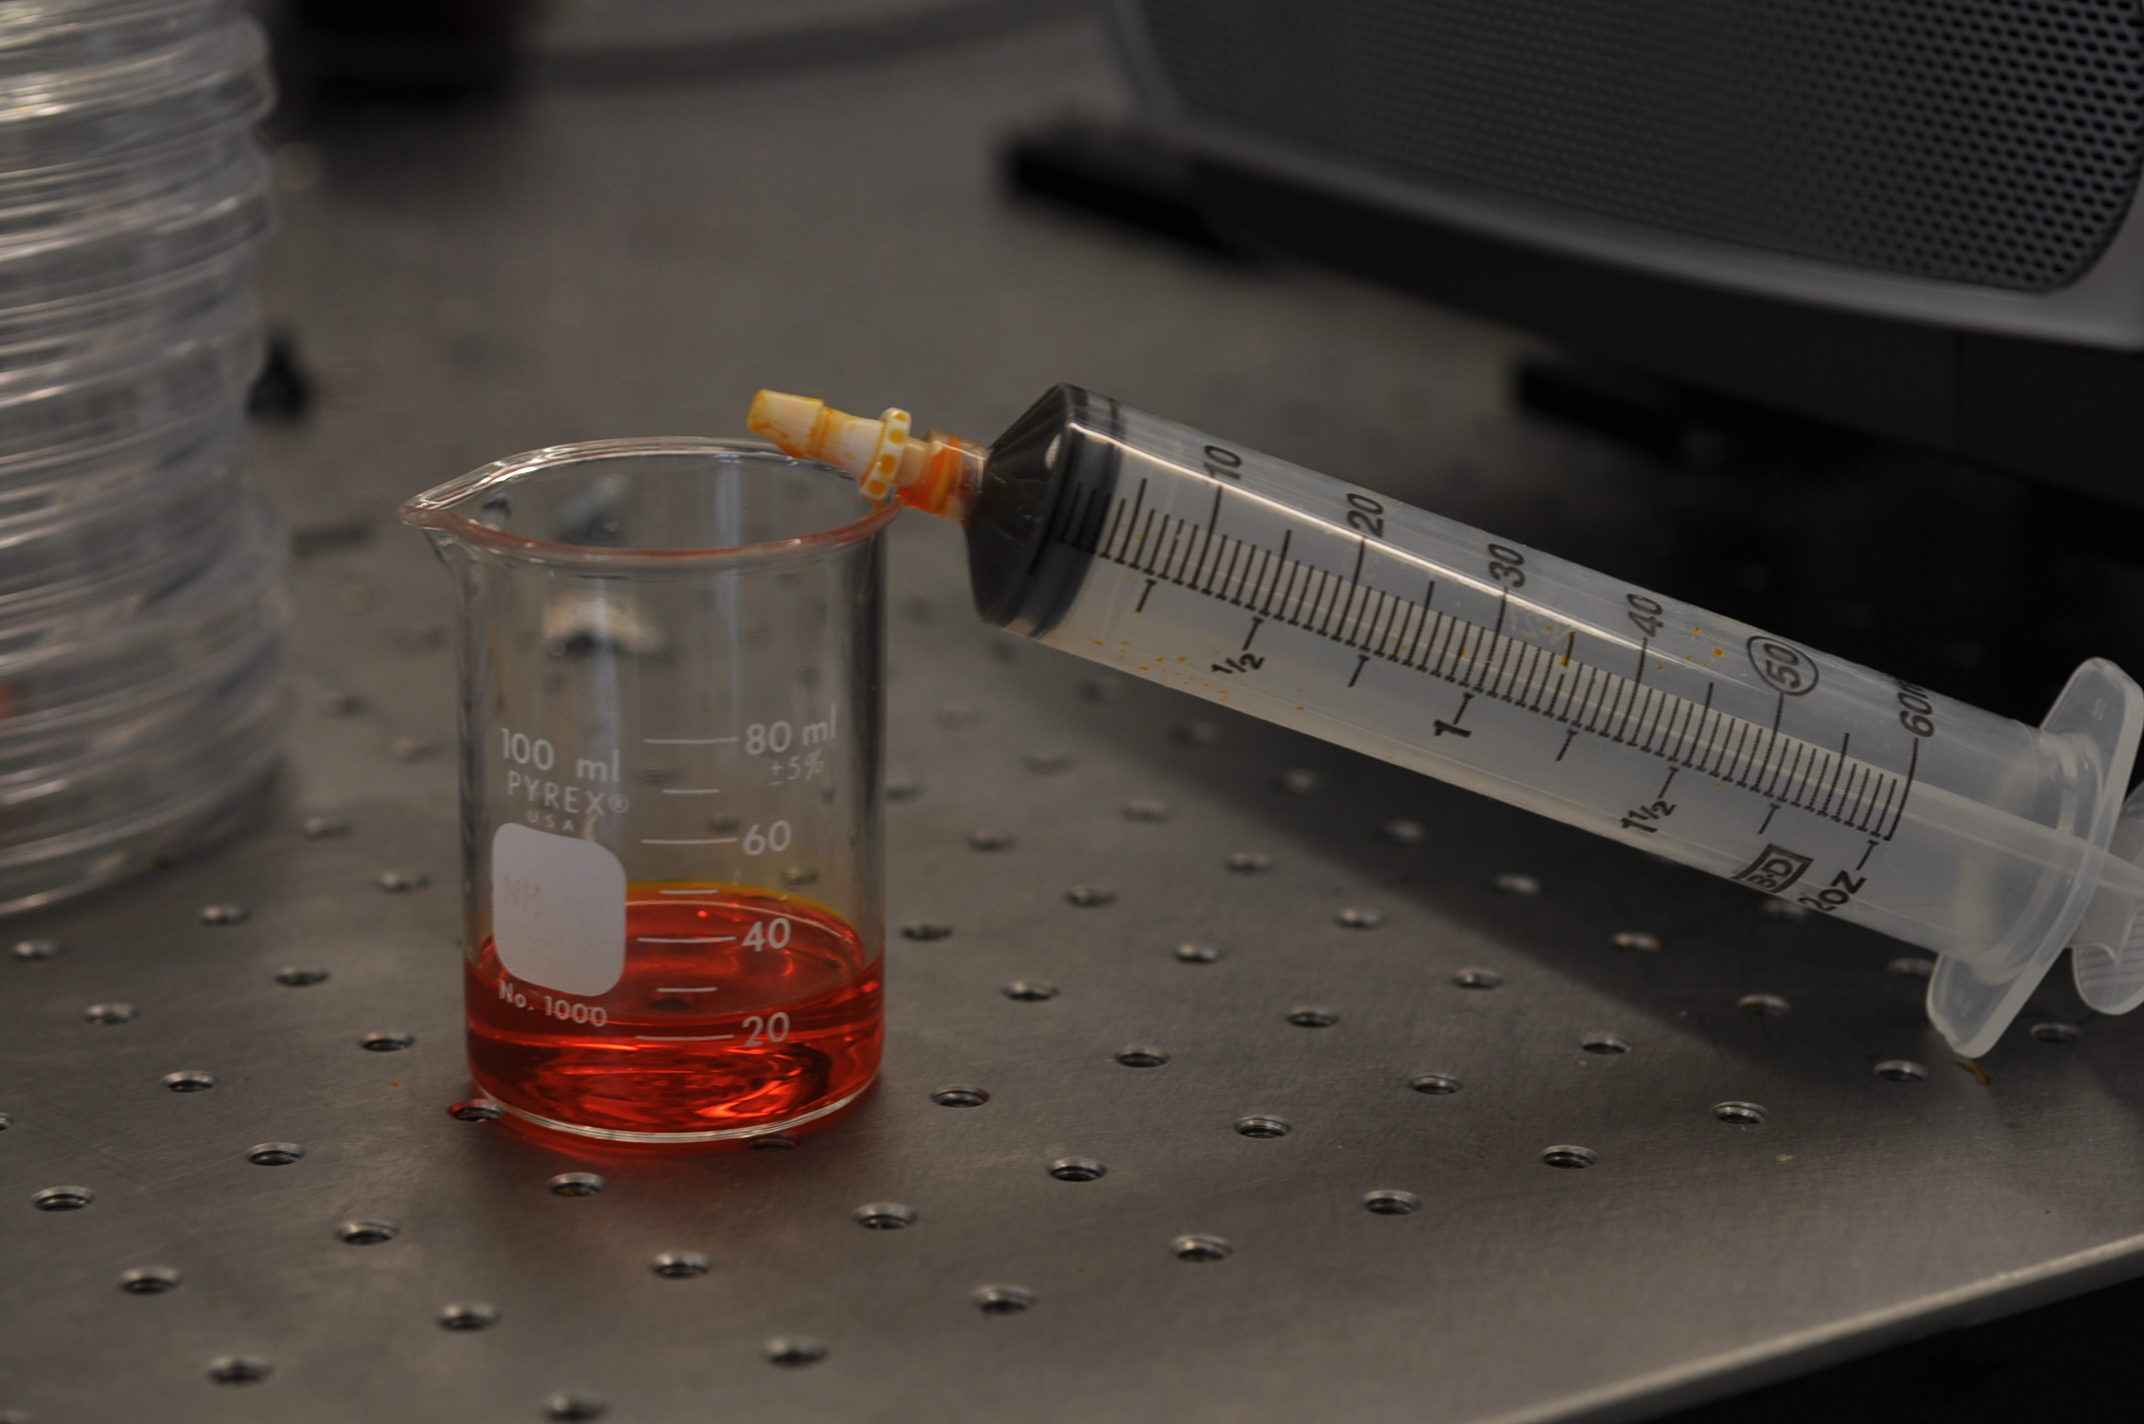
\includegraphics[width=0.3\textwidth]{pre5r.jpg}}\\
            \\
        \end{tabularx}

        \begin{tabularx}{\textwidth}{ XXX }
        \item \textbf{Step 2} : \textbf{Add} material carefully with a small syringe. When the liquid level is just above the 
            printing panel, it's ready to print.
            &\raisebox{-0.95\height}{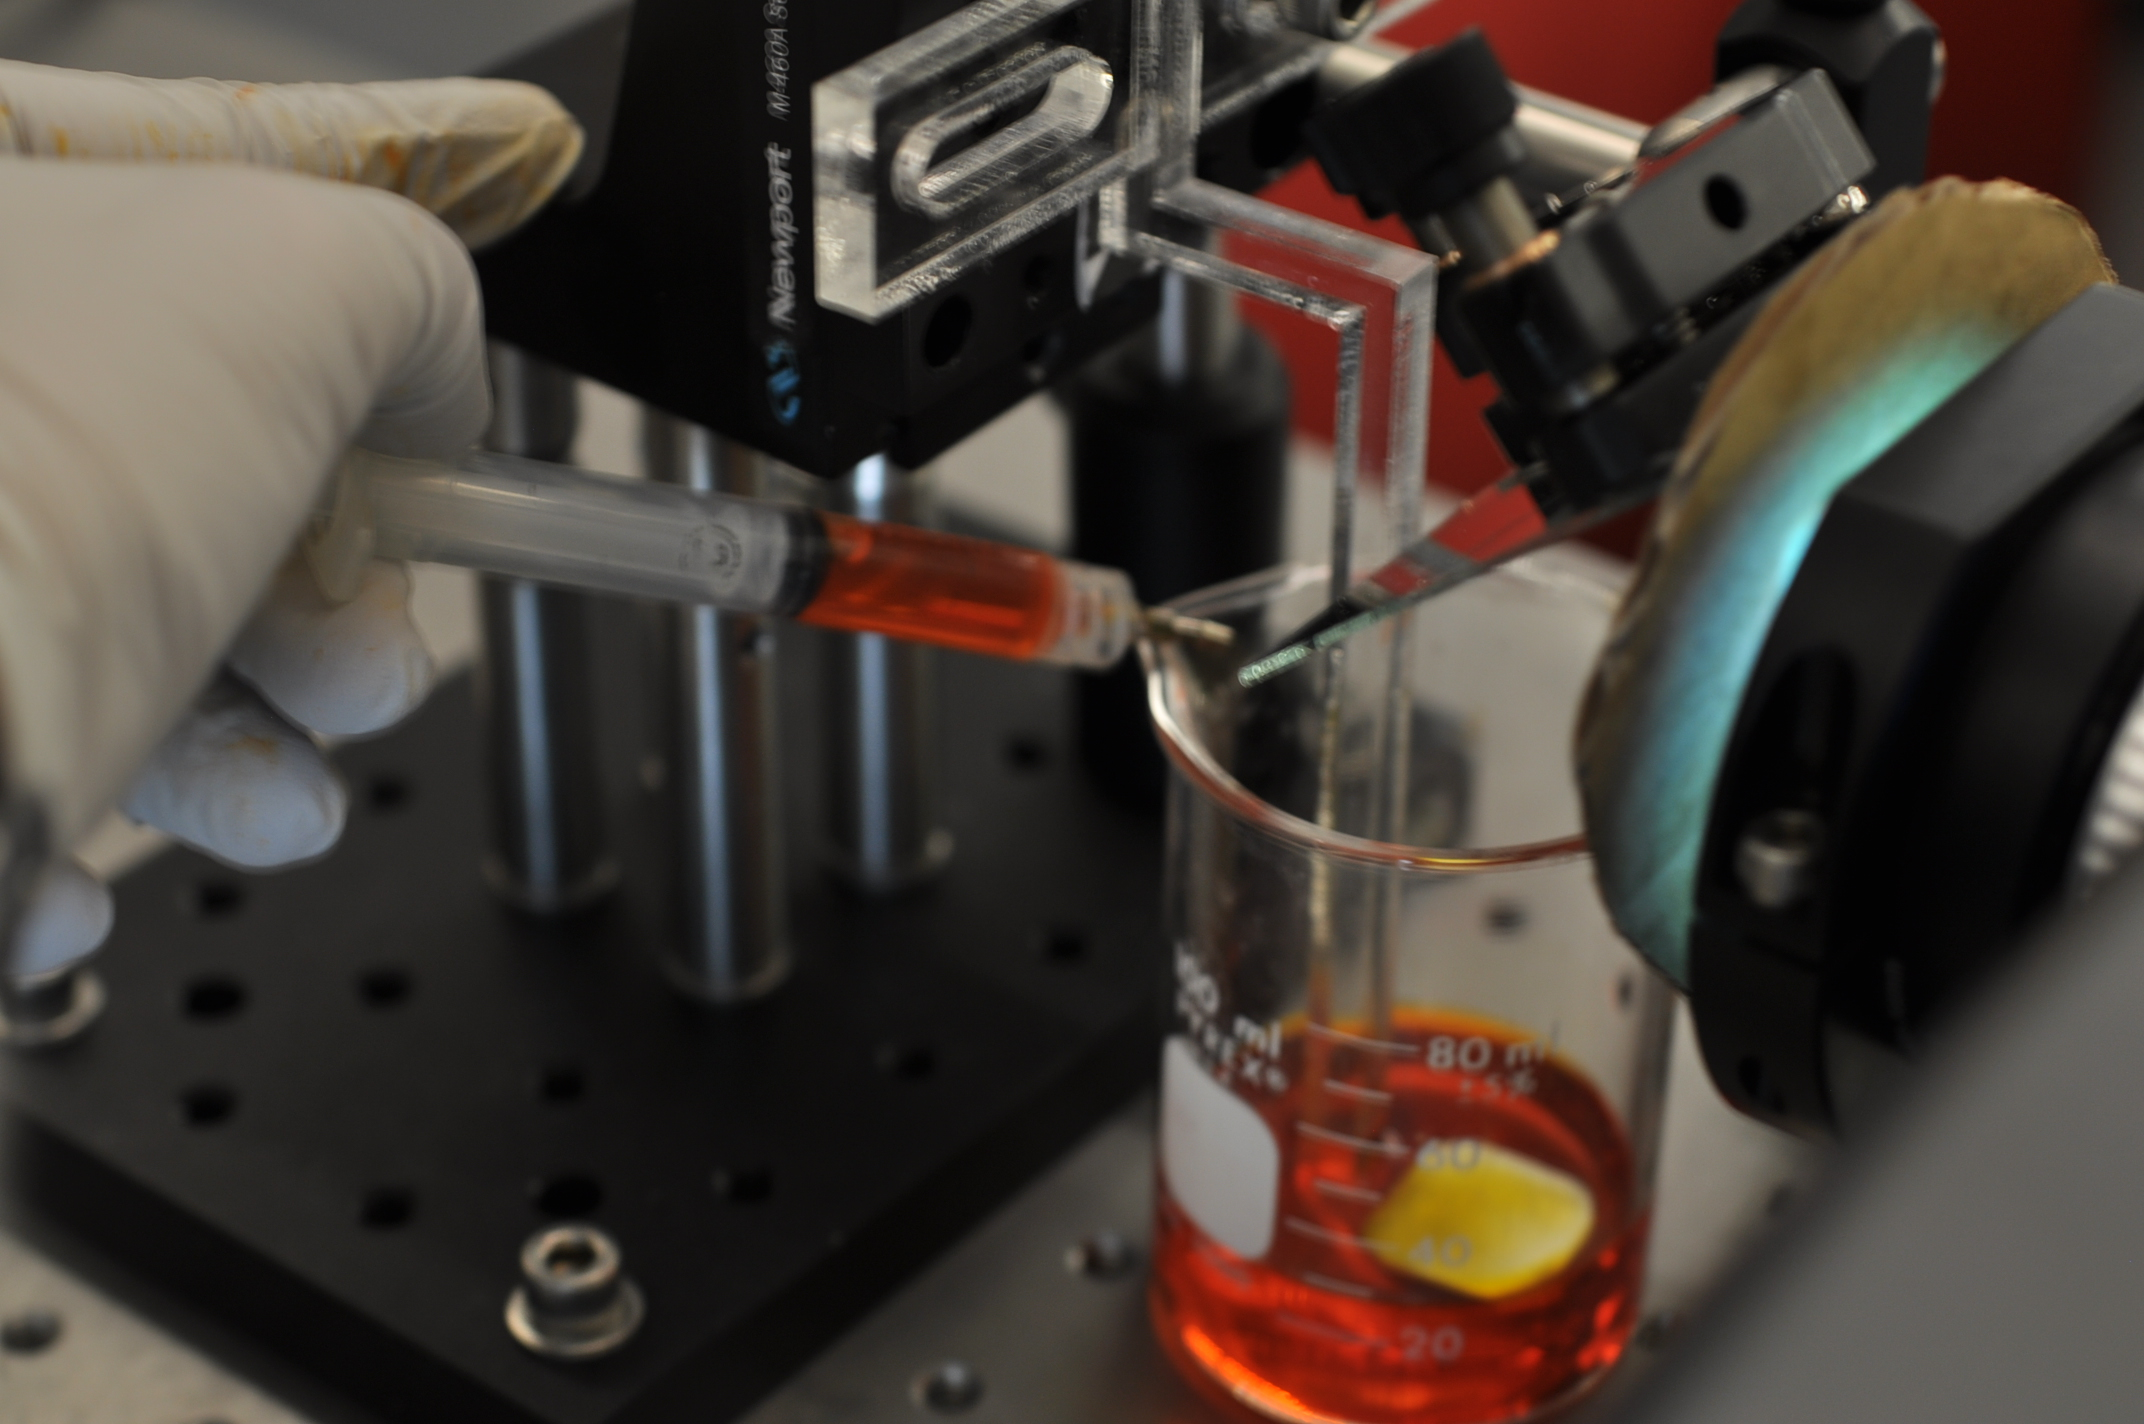
\includegraphics[width=0.3\textwidth]{pre6l.jpg}}
            &\raisebox{-0.95\height}{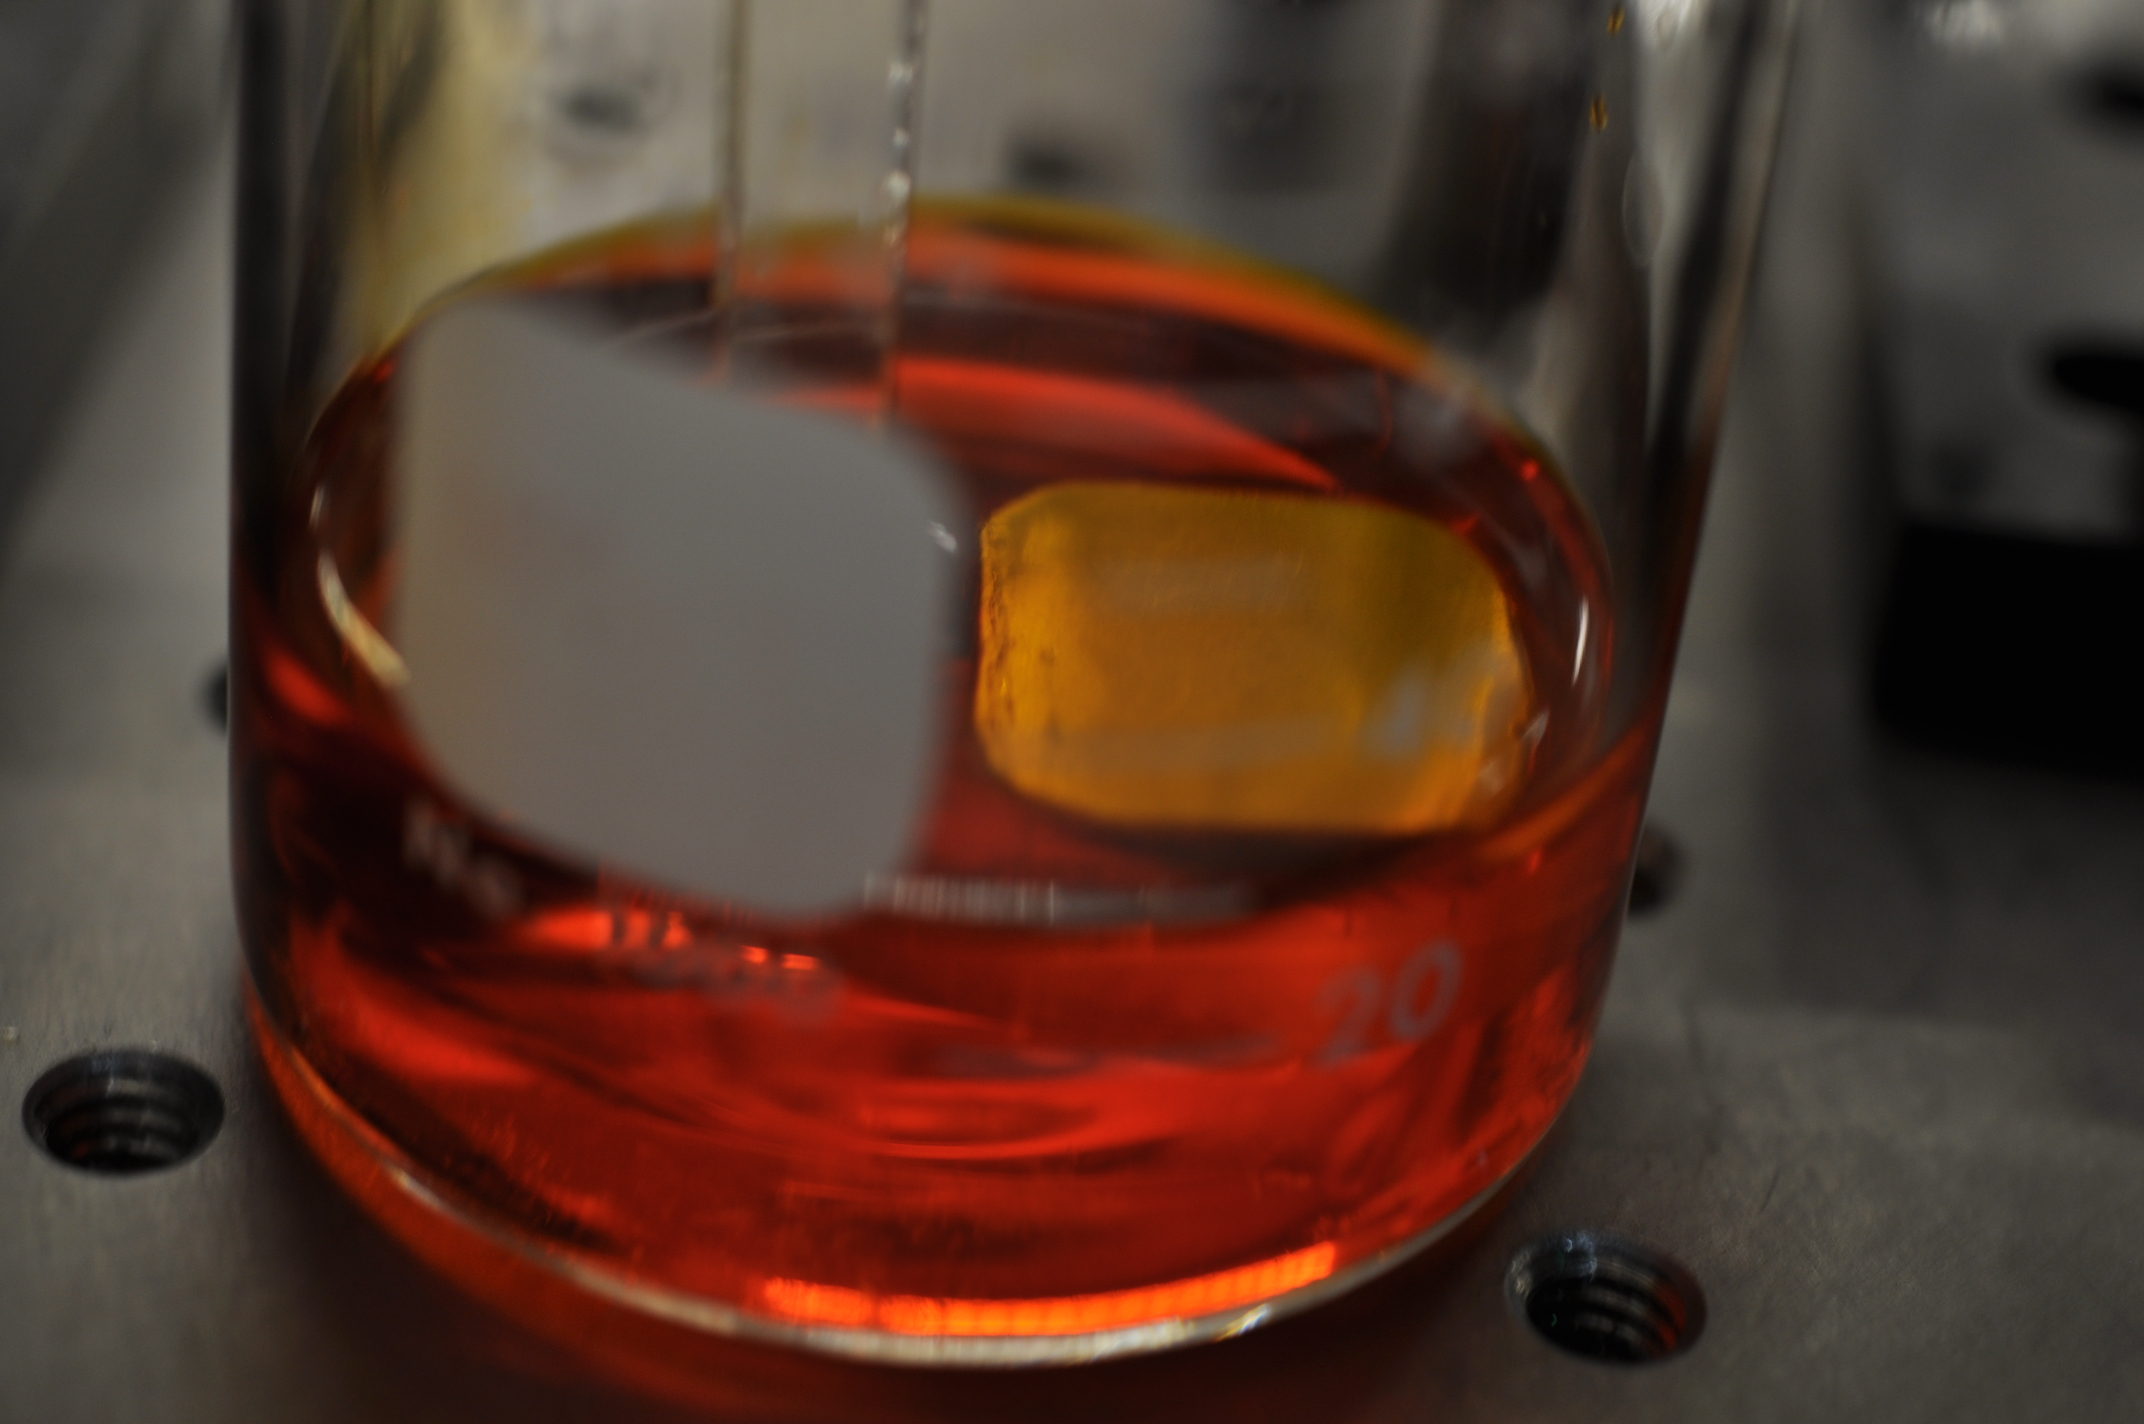
\includegraphics[width=0.3\textwidth]{pre6r.jpg}}\\
            \\
        \end{tabularx}

        \begin{tabularx}{\textwidth}{ XXX }
        \item \textbf{Step 3} : \textbf{Set} the image you need to print as desktop background. \textbf{Open} 'voice.py' and input the 
            parameters. Then Go back to the printer immediately. See more in Section \ref{sec:software}.
            &\raisebox{-0.95\height}{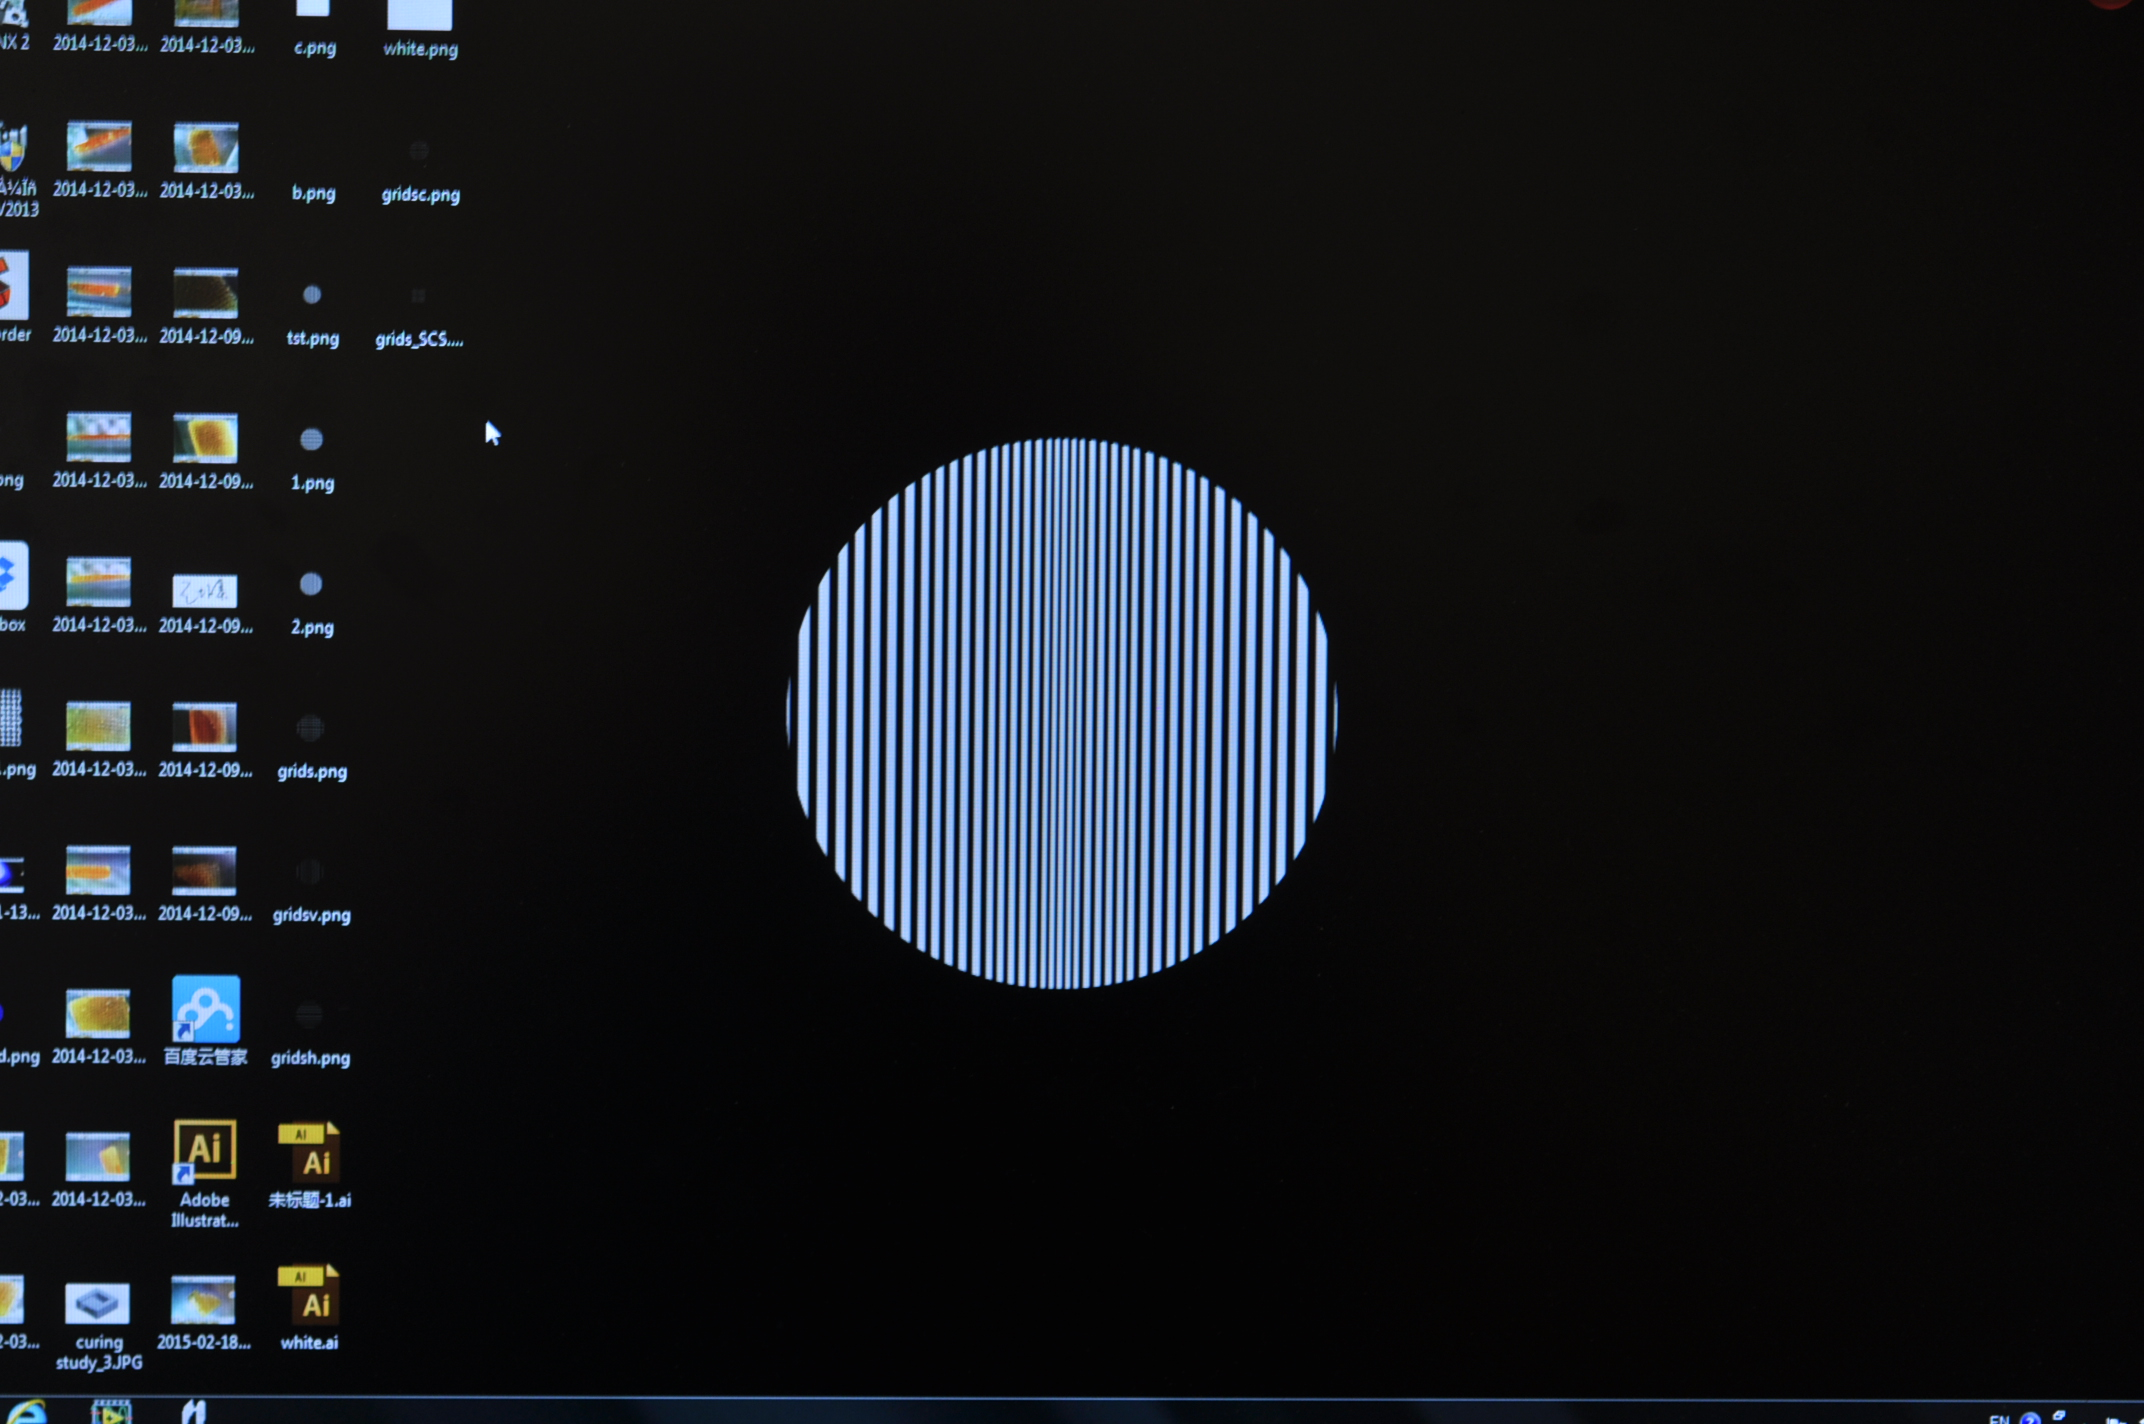
\includegraphics[width=0.3\textwidth]{prt1l.jpg}}
            &\raisebox{-0.95\height}{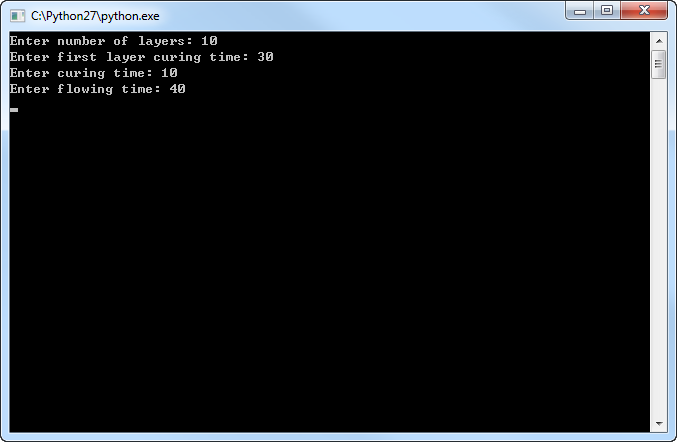
\includegraphics[width=0.3\textwidth]{prt1r.png}}\\
            \\
        \end{tabularx}

        \begin{tabularx}{\textwidth}{ XXX }
        \item \textbf{Step 4} : Follow the voice instruction. When hearing 'Projecting', \textbf{open} the light barrier. 
            After several seconds set in previus step, you will hear 'finish' which means you should \textbf{close} the barrier.
            &\raisebox{-0.95\height}{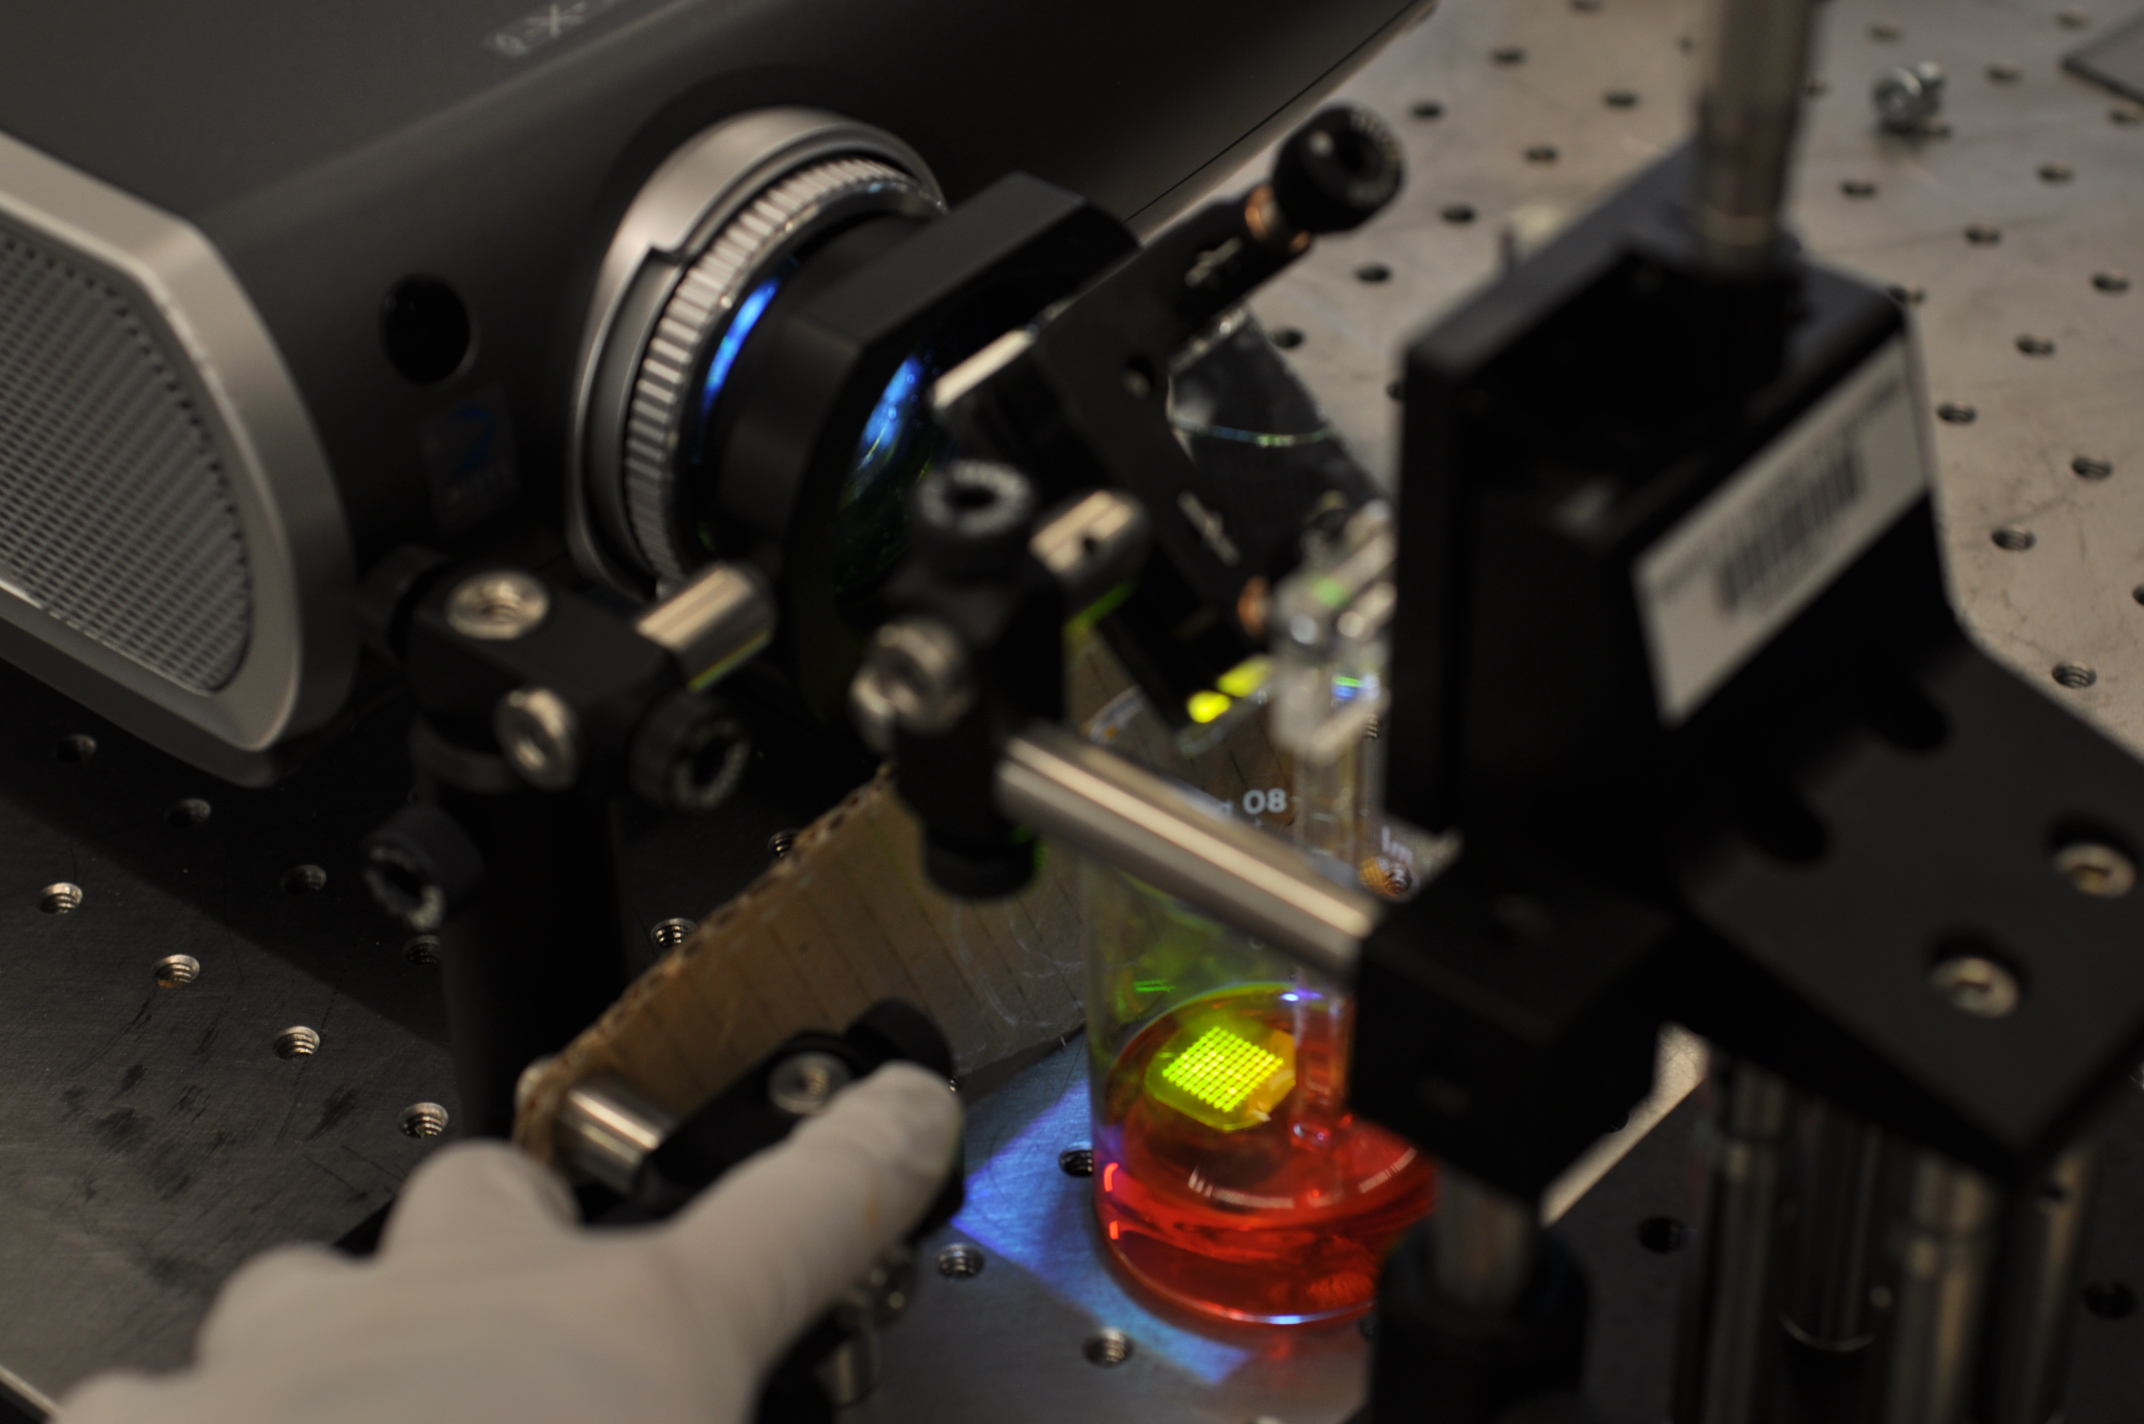
\includegraphics[width=0.3\textwidth]{prt2l.jpg}}
            &\raisebox{-0.95\height}{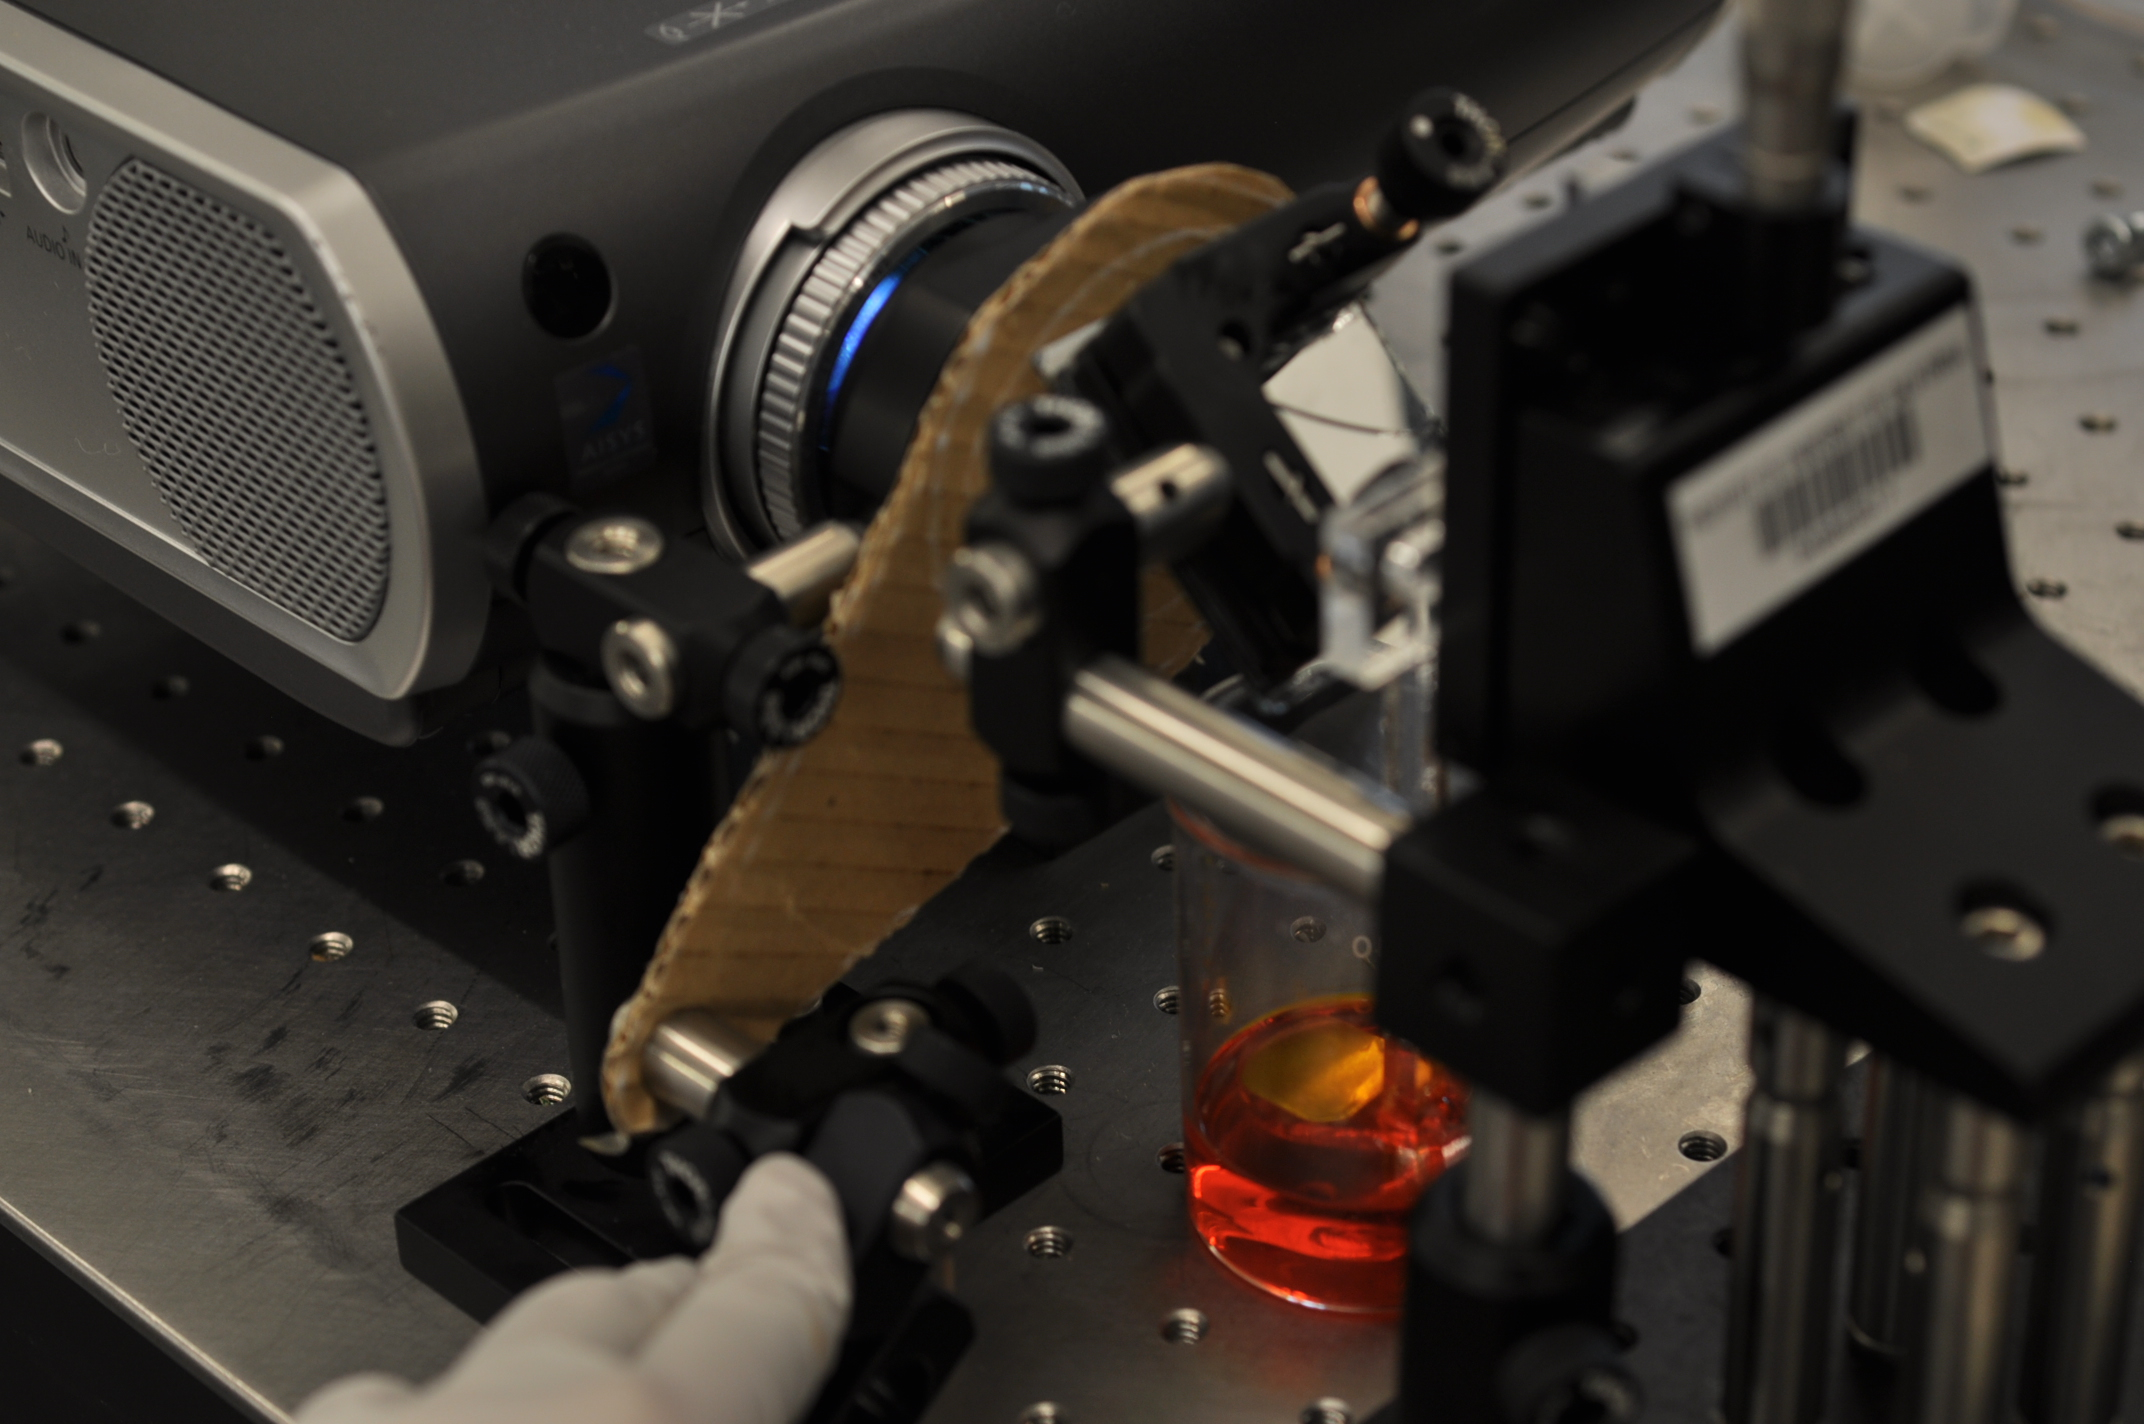
\includegraphics[width=0.3\textwidth]{prt2r.jpg}}\\
            \\
        \end{tabularx}

        \begin{tabularx}{\textwidth}{ XXX }
        \item \textbf{Step 5} : When hearing 'rotate the knob counterclockwise / clockwise to XX', just follow it and rotate the knob 
            on linear stage to the number you heard in right direction. See \ref{sec:software} and \ref{sec:linear_stage} 
            for more information.
            &\raisebox{-0.95\height}{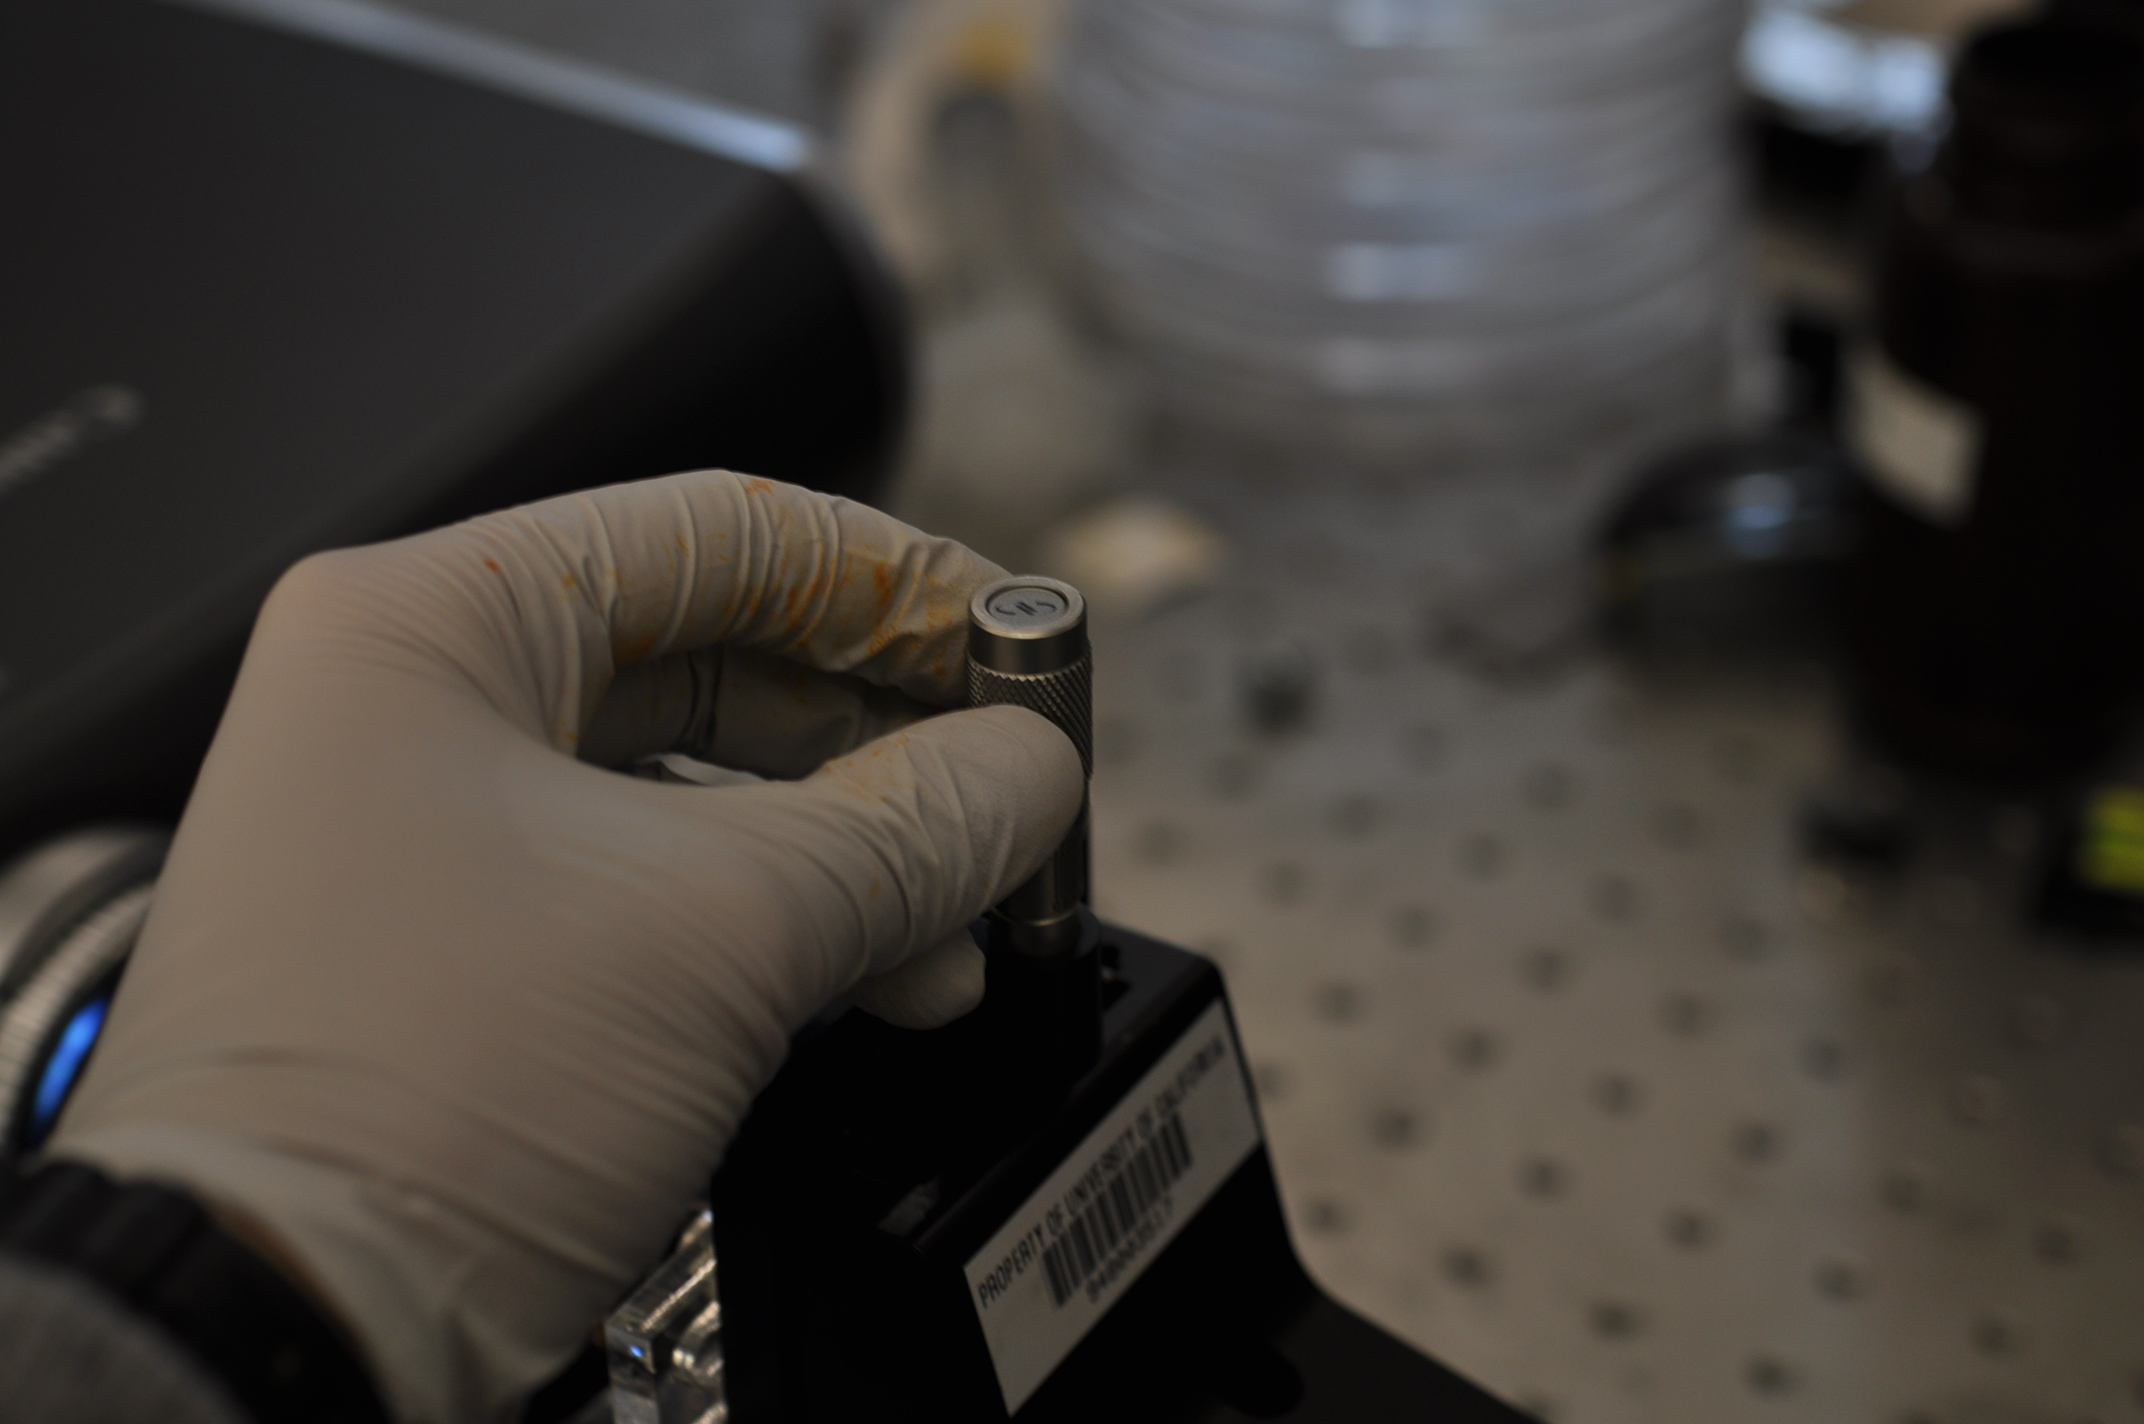
\includegraphics[width=0.3\textwidth]{prt3l.jpg}}
            &\raisebox{-0.95\height}{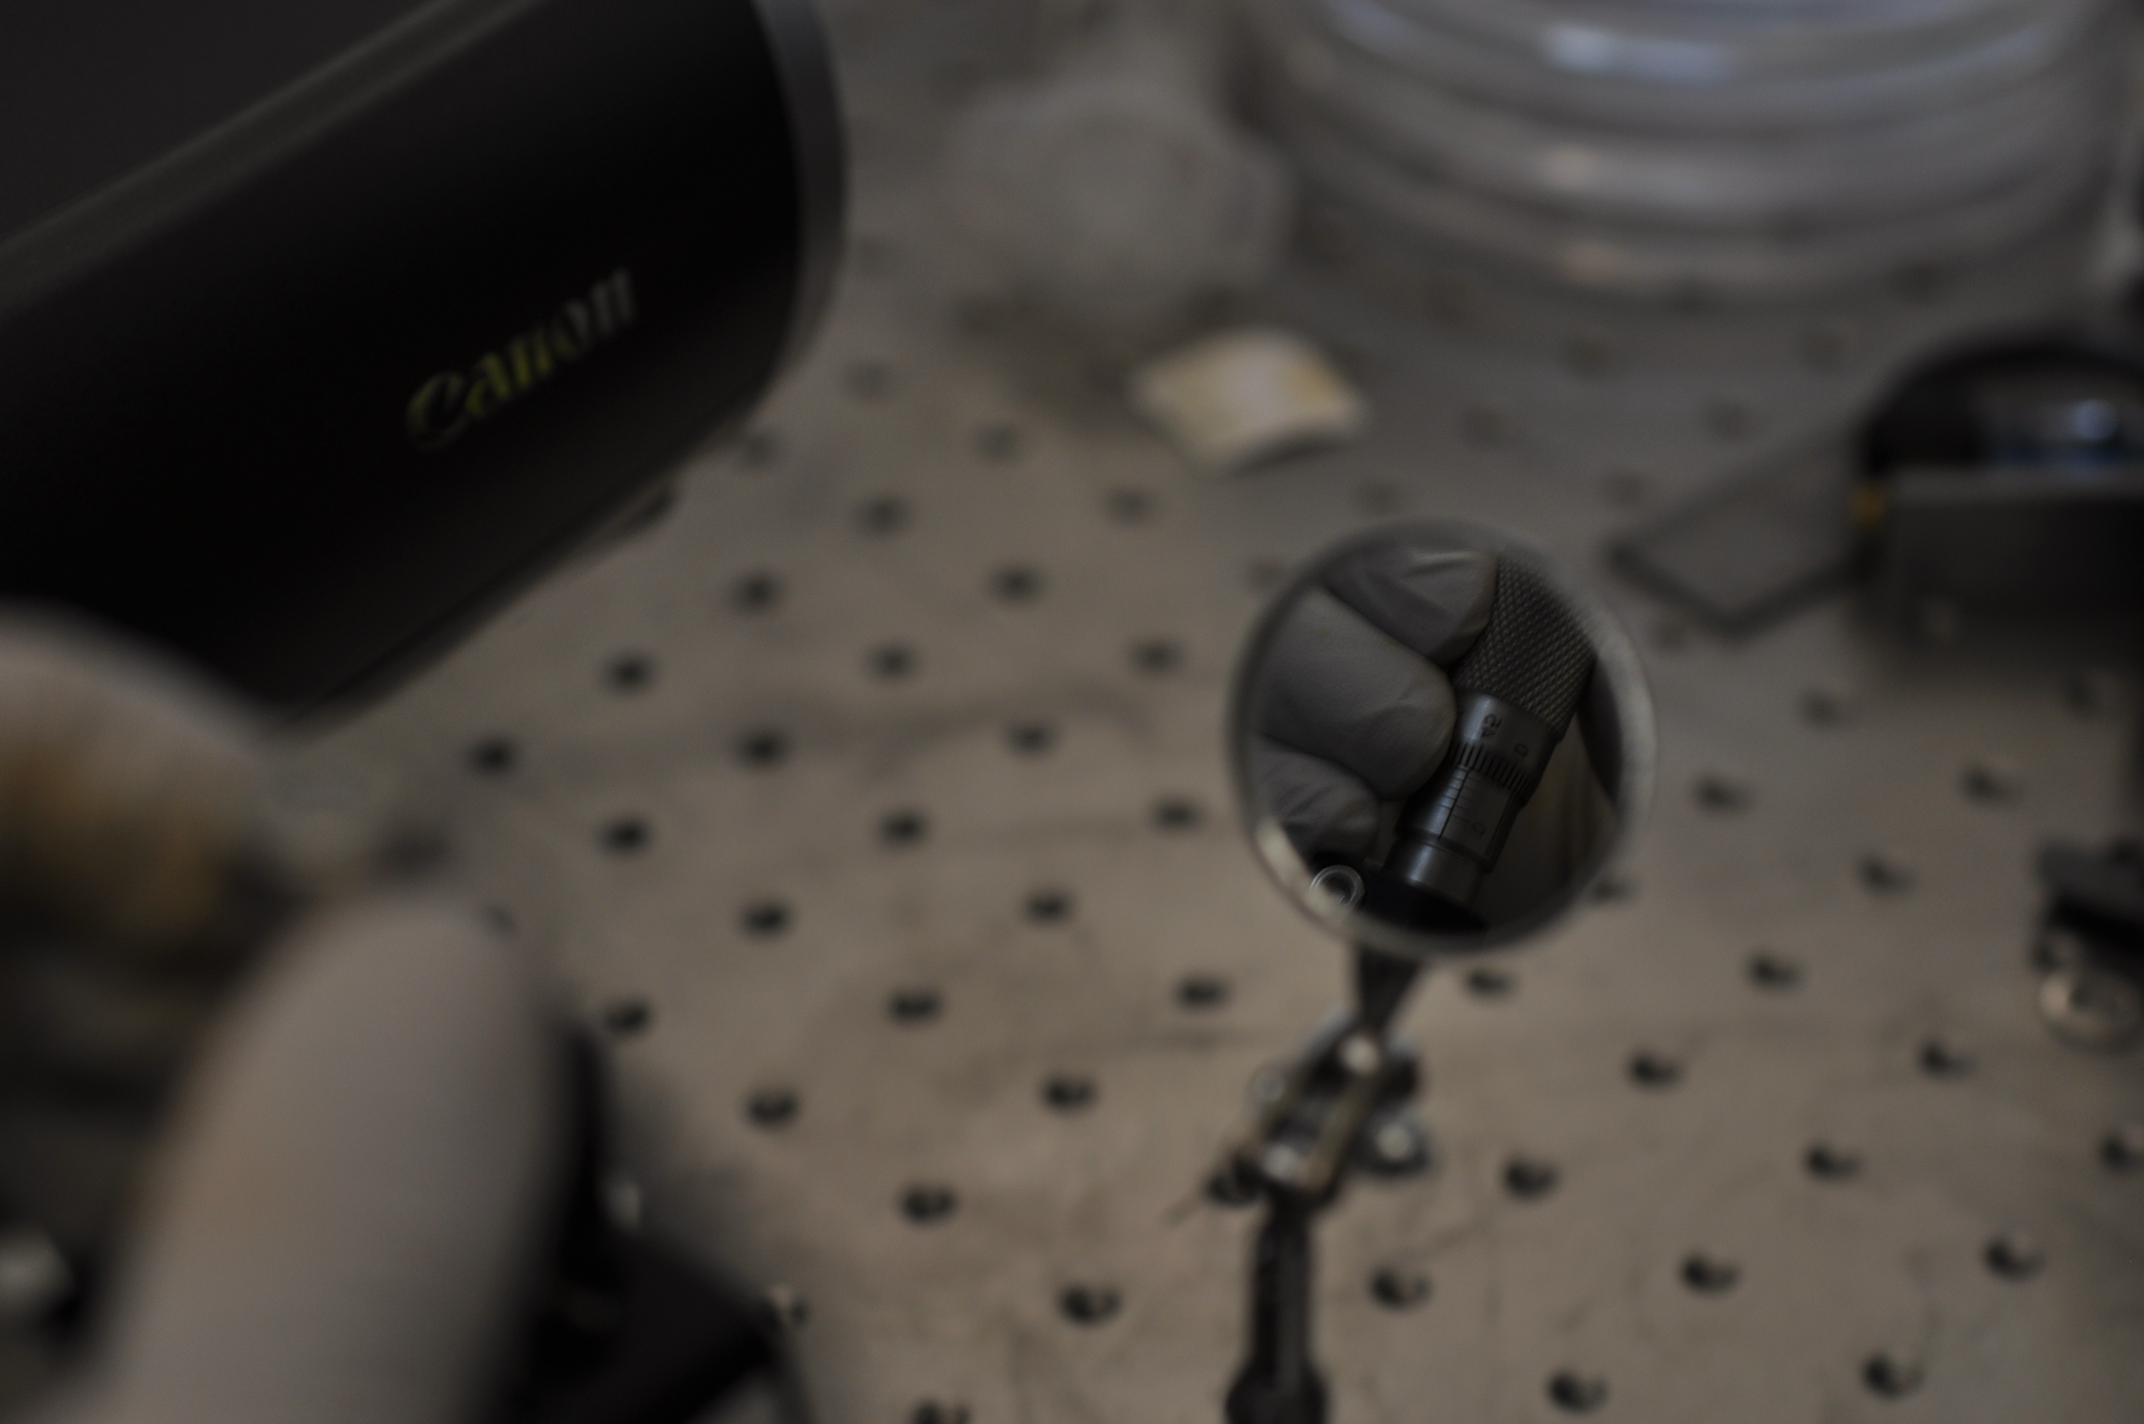
\includegraphics[width=0.3\textwidth]{prt3r.jpg}}\\
            \\
        \end{tabularx}

        \begin{tabularx}{\textwidth}{ XXX }
        \item \textbf{Step 6} : \textbf{Repeat} step 4 \& 5. When hearing 'Fabrication finish', the sample is done. \textbf{Take away} 
            the stage and \textbf{cut} the sample off carefully with a blade.
            &\raisebox{-0.95\height}{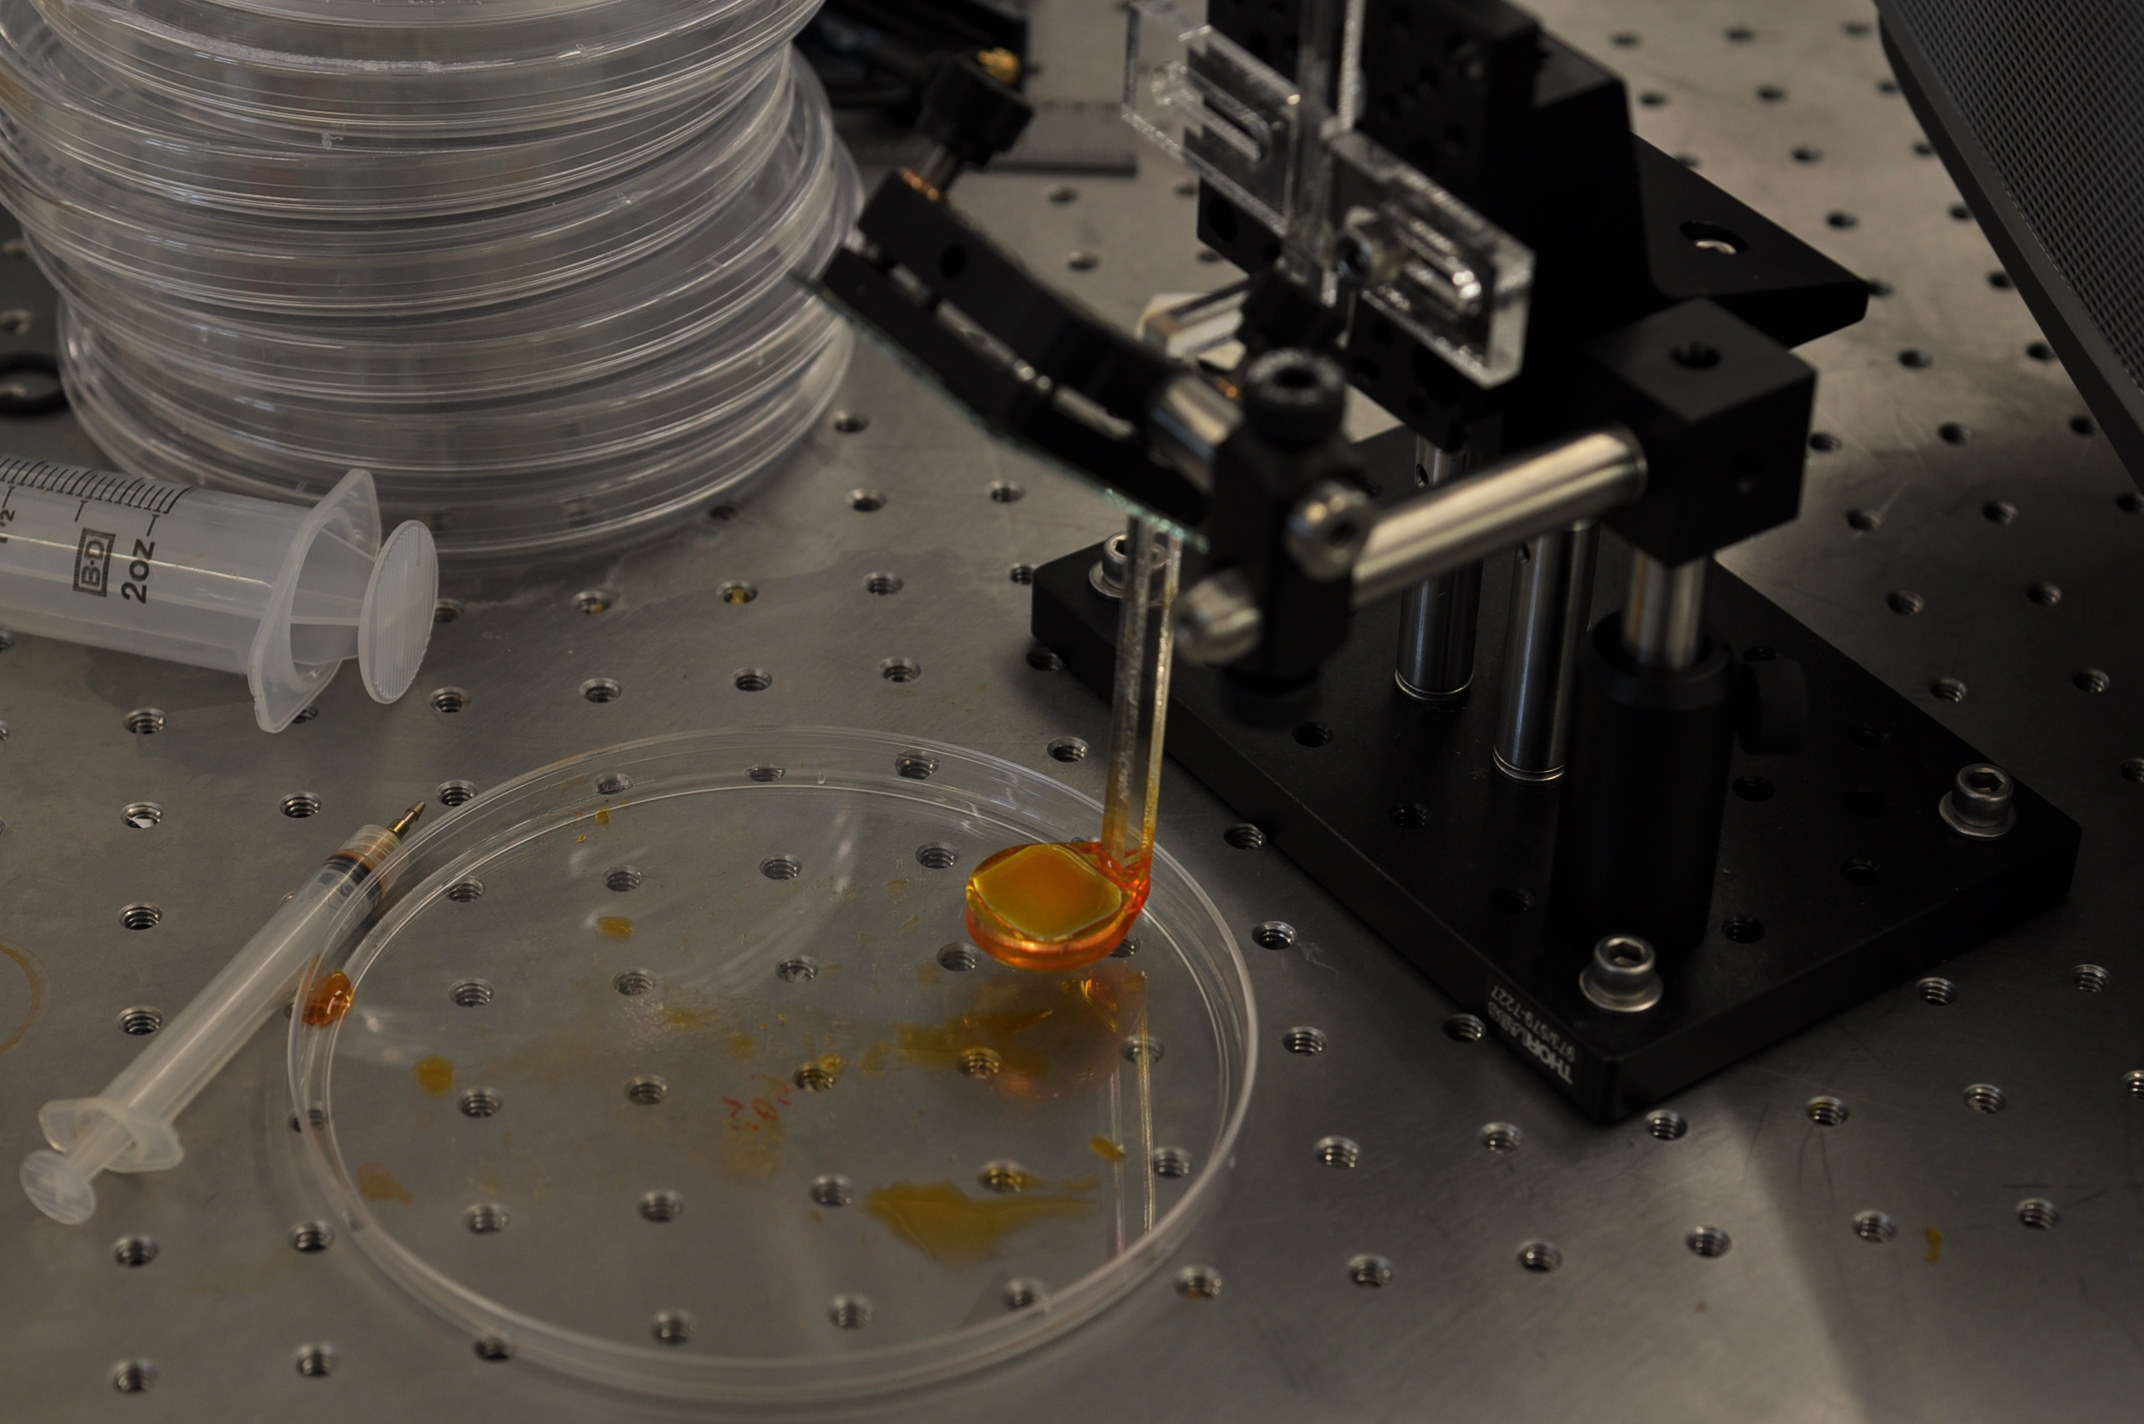
\includegraphics[width=0.3\textwidth]{prt4l.jpg}}
            &\raisebox{-0.95\height}{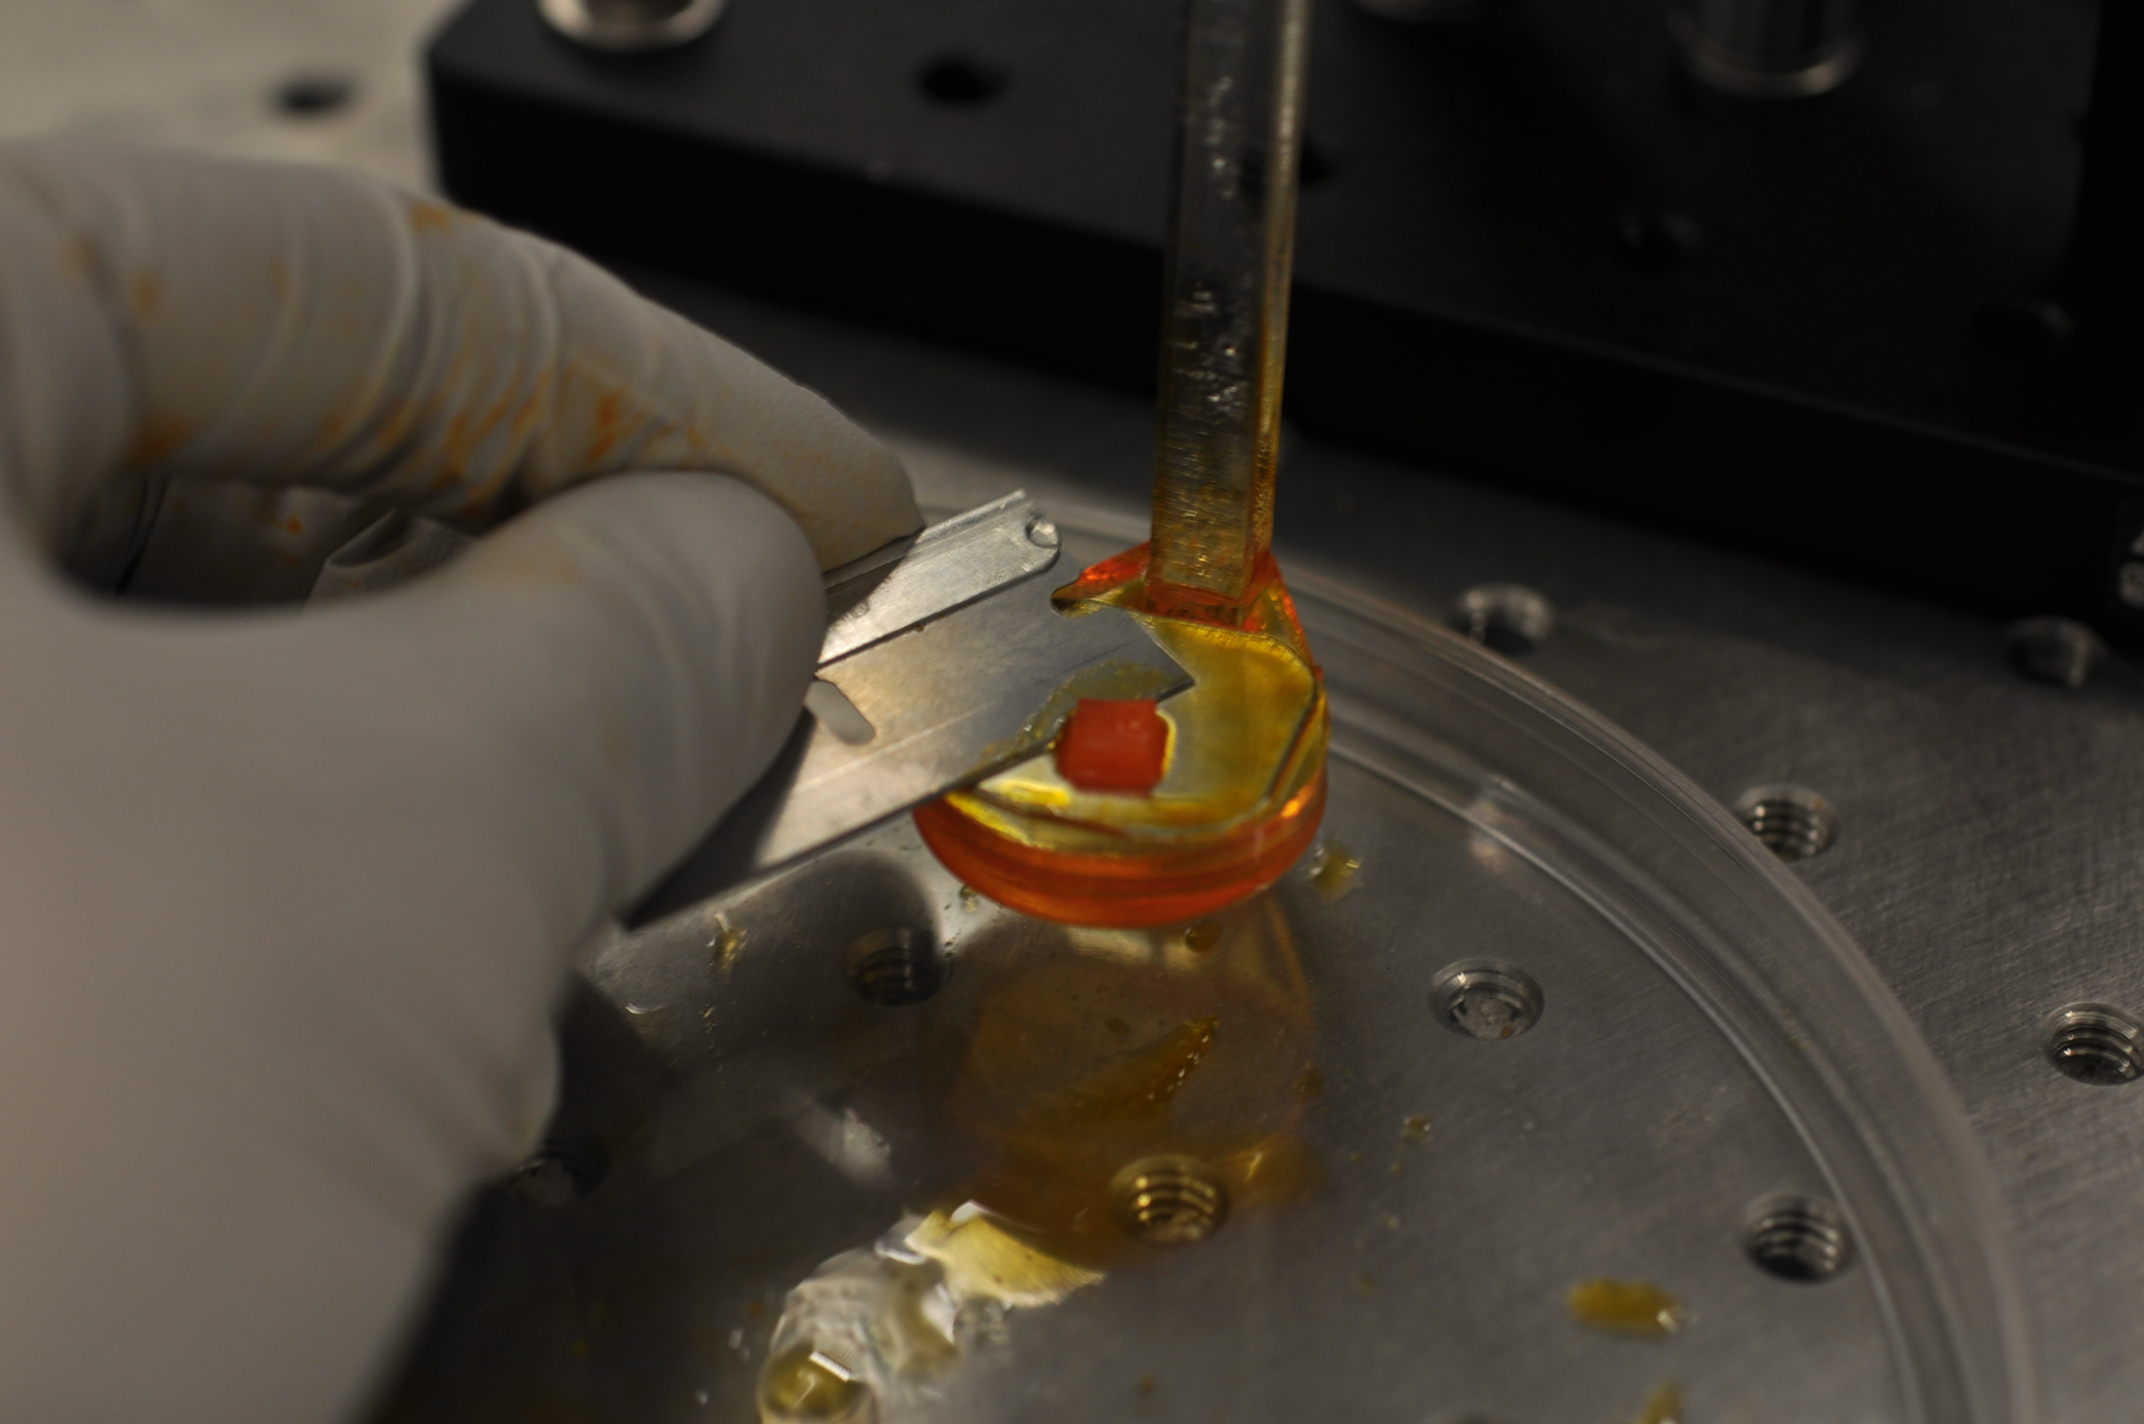
\includegraphics[width=0.3\textwidth]{prt4r.jpg}}\\
            \\
        \end{tabularx}

        \begin{tabularx}{\textwidth}{ XXX }
        \item \textbf{Step 7} : \textbf{Clean up} the sample holder with isopropanol then \textbf{put} the stage back.
            % &\raisebox{-\height}{\includegraphics[width=0.3\textwidth]{prt5l.jpg}}
            % &\raisebox{-\height}{\includegraphics[width=0.3\textwidth]{prt5r.jpg}}\\
        \end{tabularx}
\end{itemize}

% \subsection{Cleaning}\label{sec:cleaning}
% bla

\appendix
\section{Appendix}\label{sec:appendix}
\subsection{Linear stage}\label{sec:linear_stage}



\subsection{Convex lens adjustment}\label{sec:convex_lens_adjustment}
\begin{itemize}
        \begin{tabularx}{\textwidth}{ Xc }
        \item The \textit{knob X} and \textit{knob Z} can \textbf{adjust} the position of the convex lens in 
            \textit{X, Z dimension} as well as \textit{the rotation in X, Z axis}. And the \textit{screw Y} can 
            \textbf{adjust} the lens' position in \textit{Y dimension}. You should make sure that the lens is 
            central and vertical with the \textit{main optical axis}, which means it should be parallel and aligned 
            with the \textit{imaging lens of the projector}. The distance between convex and imaging lens will make 
            sense to the \textit{focal panel}. 
            &\raisebox{-\height}{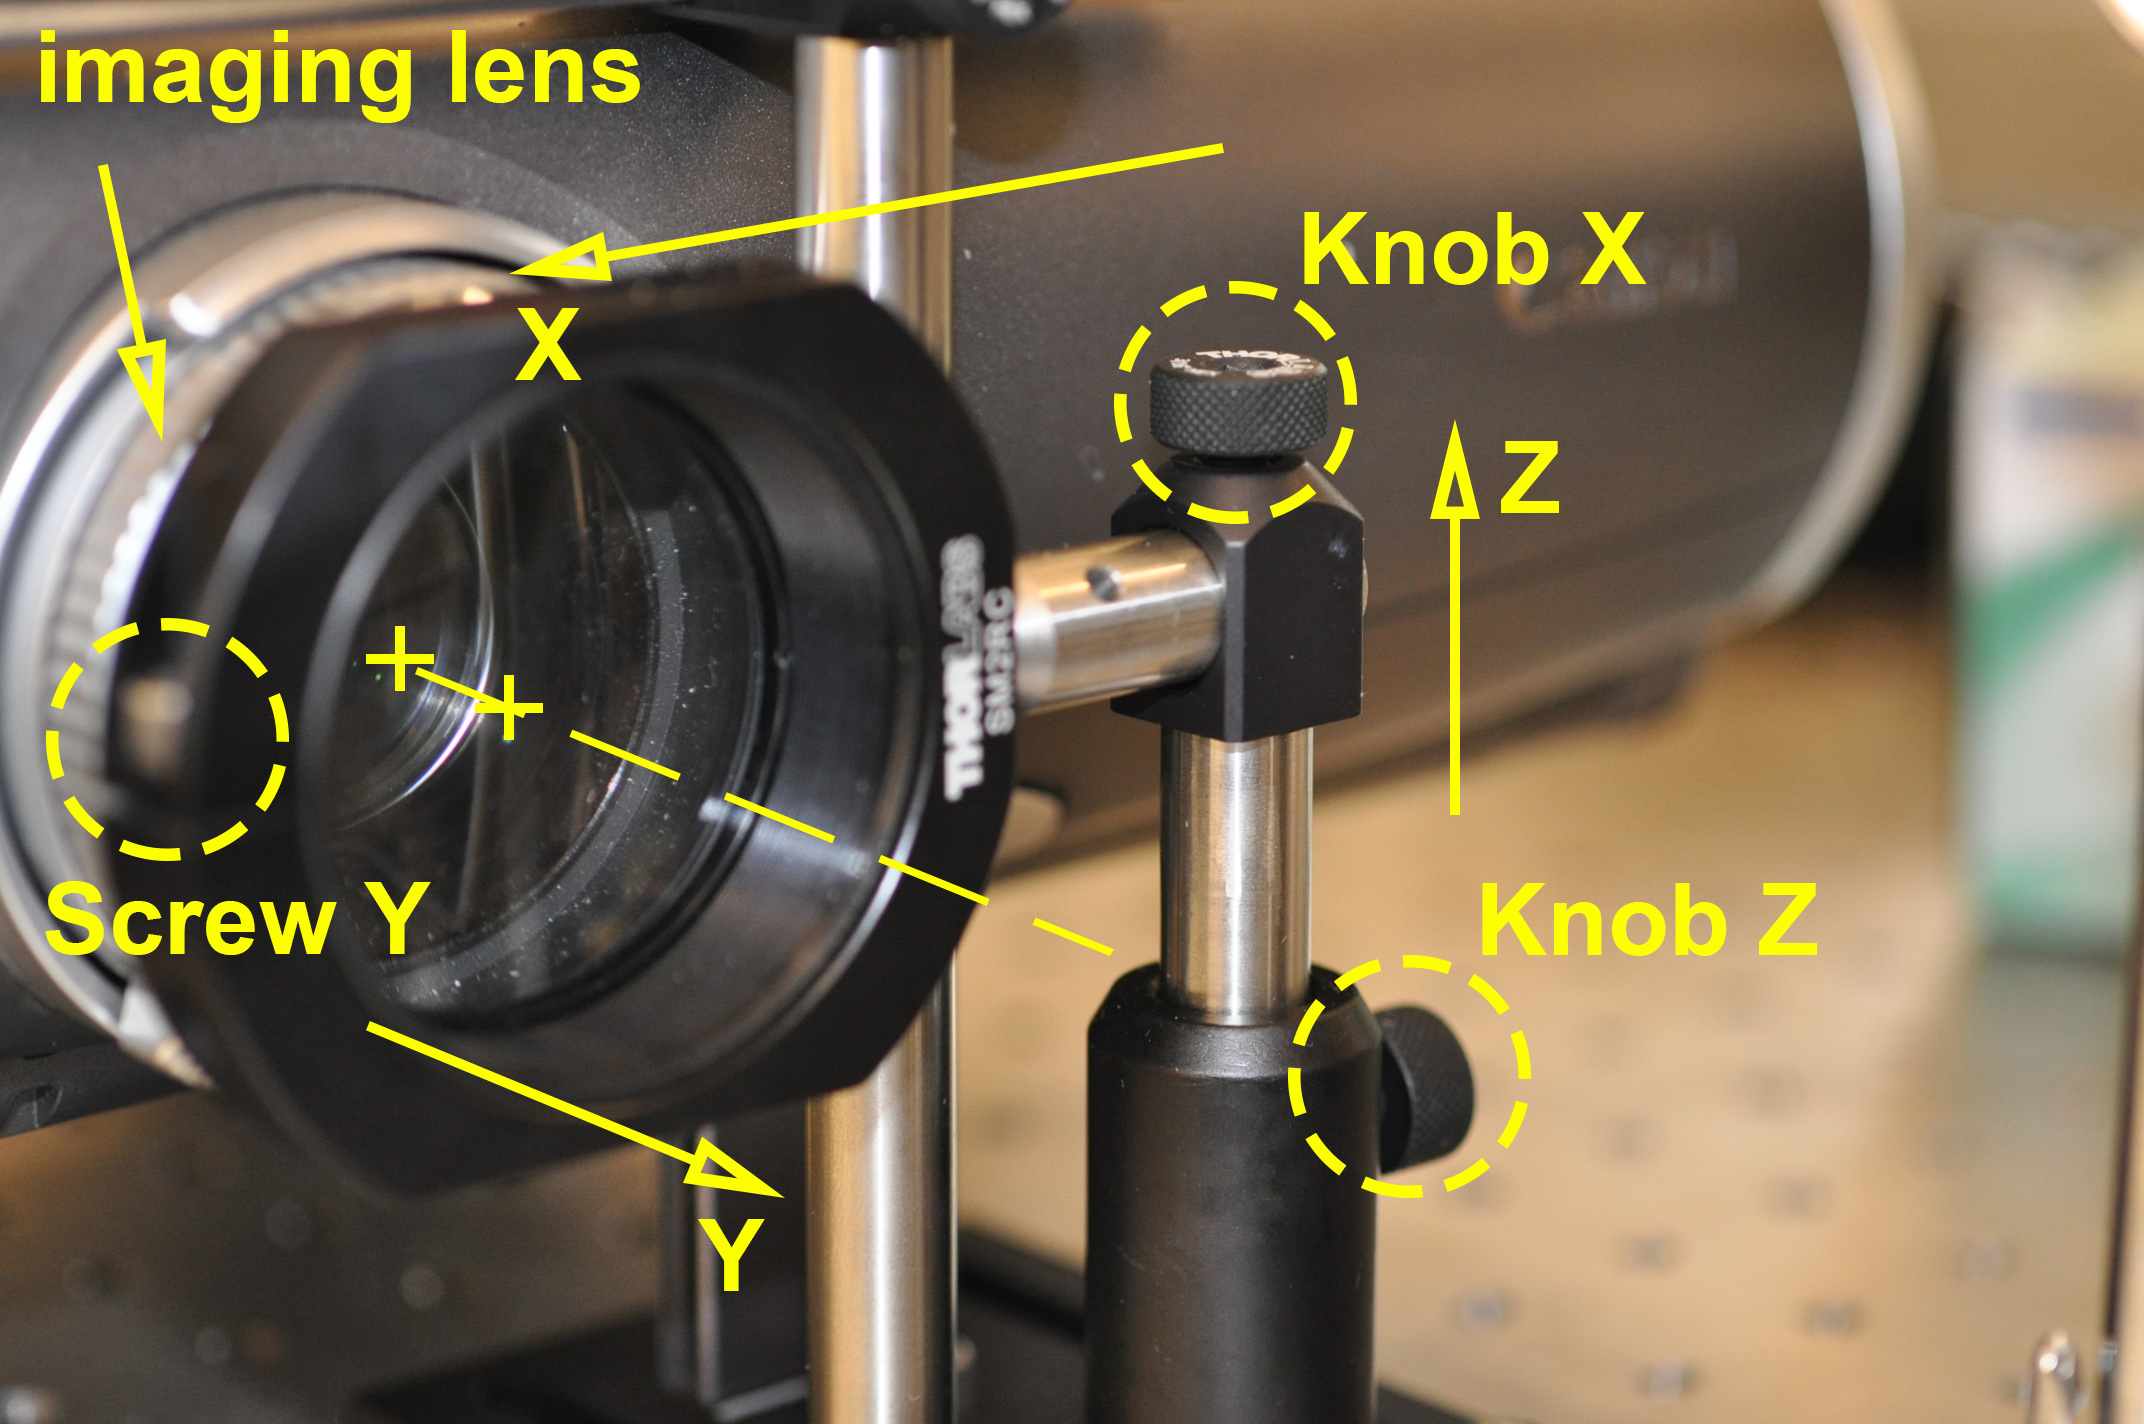
\includegraphics[width=0.33\textwidth]{lens_adjust.jpg}}\\
            \\
        \end{tabularx}
\end{itemize}

\subsection{Mirror adjustment}\label{sec:mirror_adjustment}
\begin{itemize}
        \begin{tabularx}{\textwidth}{ Xc }
        \item The \textit{knob U, V, W} can \textbf{adjust} the position and the rotation in \textit{three dimensions}. 
            First you should \textbf{adjust the mirror coarsely} and \textbf{let} the image projected on the sample holder. 
            Not being in the center is OK, you can \textbf{make fine adjustment} in the next step. 
            &\raisebox{-\height}{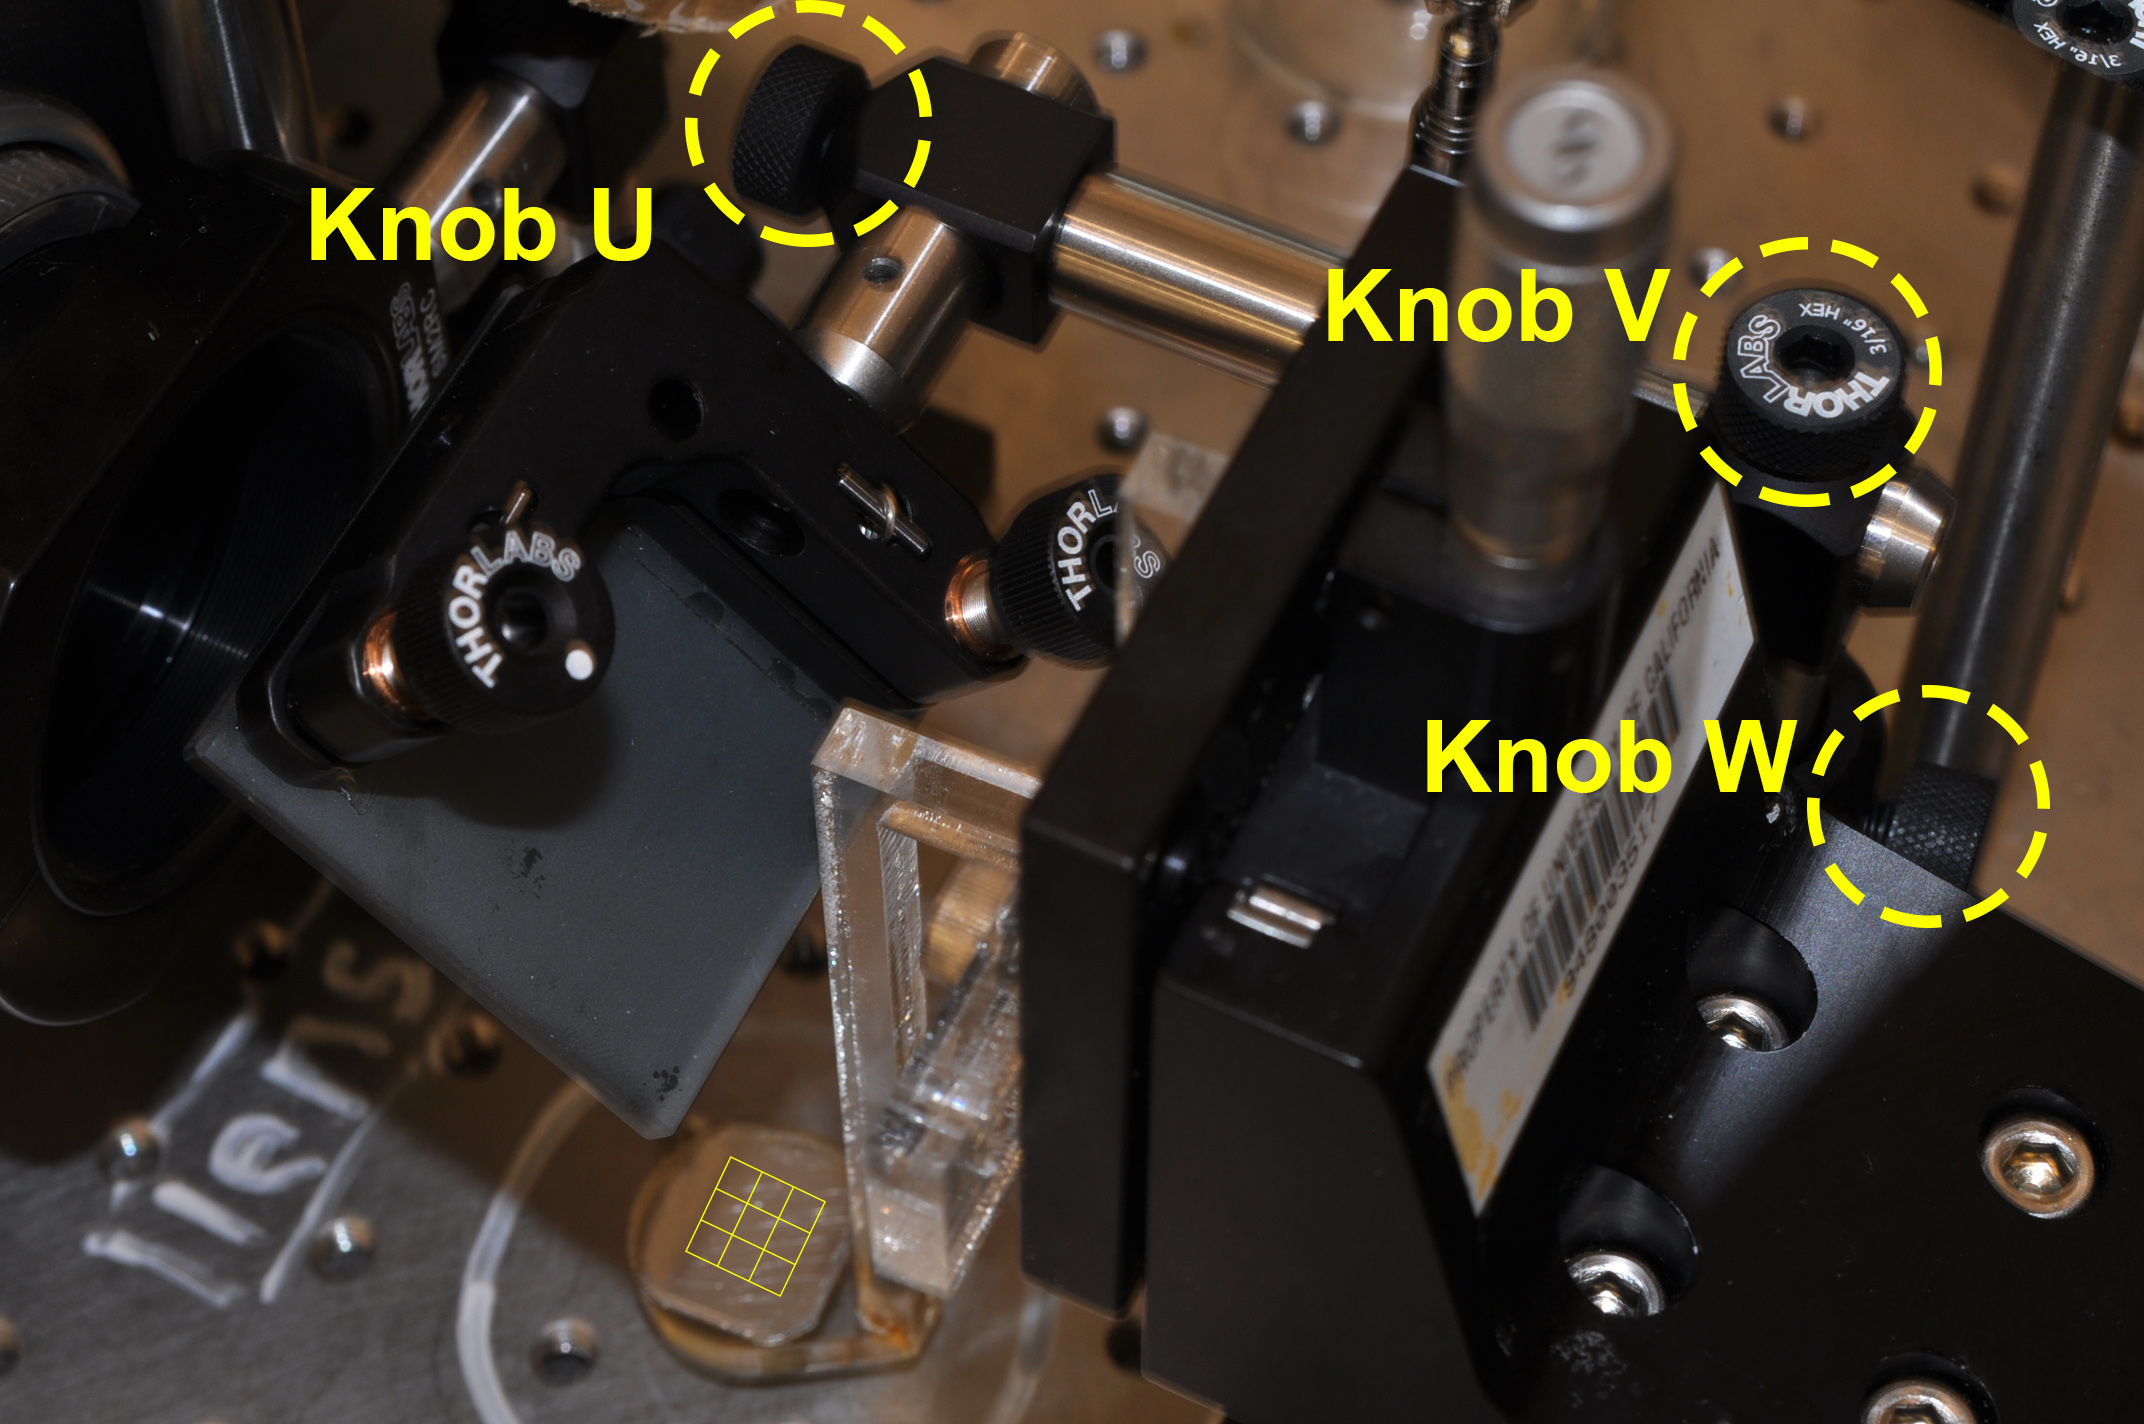
\includegraphics[width=0.33\textwidth]{mirror_adjustr.jpg}}\\
            \\
        \end{tabularx}

        \begin{tabularx}{\textwidth}{ Xc }
        \item Then you need to do the \textit{fine adjustment}. The \textit{knob A} can \textbf{rotate} the mirror and 
            \textbf{let the image move} in \textit{Y axis}. The \textit{knob B} can \textbf{rotate} the mirror too and 
            \textbf{let the image move} in \textit{X axis}. So you just need to rotate the knob and make the image pojected 
            in the center of the sample holder. 
            &\raisebox{-\height}{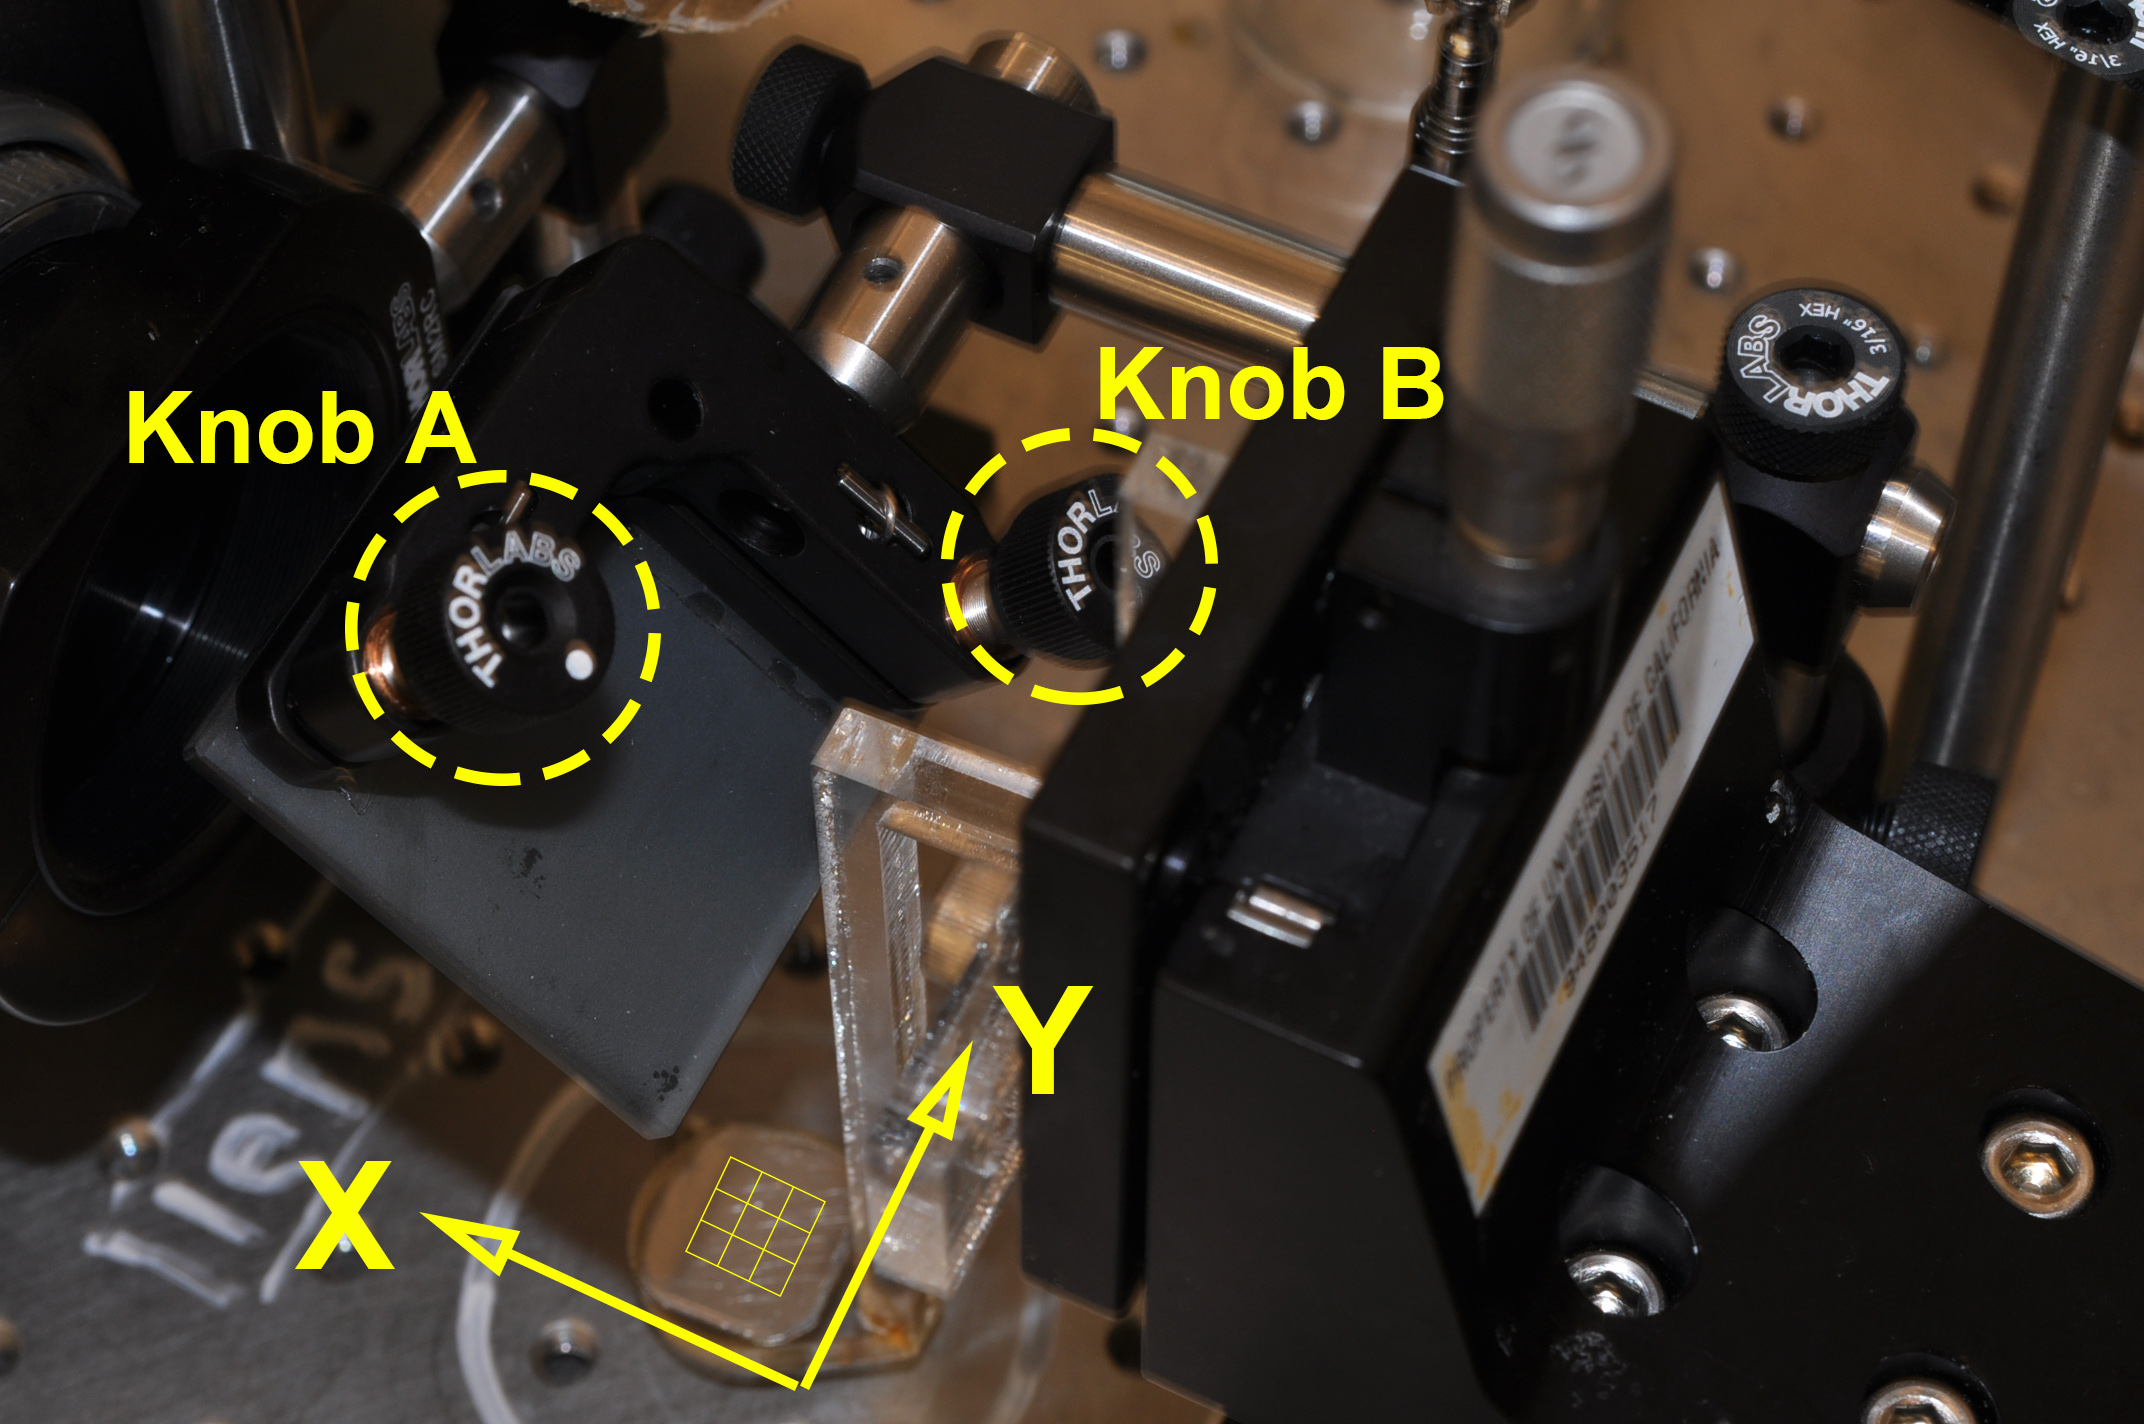
\includegraphics[width=0.33\textwidth]{mirror_adjust.jpg}}\\
            \\
        \end{tabularx}



\end{itemize}

\end{document}
